\PassOptionsToPackage{table}{xcolor}
\documentclass[sigconf,review]{acmart}

\usepackage{booktabs}
\usepackage{amsfonts}
\usepackage{nicefrac}
\usepackage{microtype}
\usepackage{textcomp}
\usepackage{makecell}
\usepackage{graphicx}
\usepackage{amsmath}
\usepackage{amssymb}
\usepackage{array}
\usepackage{multirow}
\usepackage{makecell}
\usepackage{colortbl}
\usepackage{xspace}
\usepackage{enumitem}
\usepackage{placeins}
\usepackage{tabularx}
\usepackage{float}
\usepackage[capitalize]{cleveref}

\graphicspath{{appendix_image/}{./}}

\hypersetup{
  breaklinks=true,
  colorlinks=true
}

\crefname{section}{Sec.}{Secs.}
\Crefname{section}{Section}{Sections}
\crefname{table}{Tab.}{Tabs.}
\Crefname{table}{Table}{Tables}
\crefname{figure}{Fig.}{Figs.}
\Crefname{figure}{Figure}{Figures}

\newcommand{\dataset}{sMMC-22M\xspace}
\newcommand{\methodname}{STBoost\xspace}
\newcommand{\methodfull}{STBoost Framework)\xspace}
\newcommand{\benchmarkname}{sMMC-22M Bench\xspace}
\newcommand{\placeholder}[1]{\textcolor{blue}{[#1]}}
\newcommand{\redadd}[1]{\textcolor{red}{#1}}
\newcommand{\datasheetq}[1]{\par\noindent\textbf{#1}\enspace}
\definecolor{inhouseblue}{RGB}{225,240,255}
\definecolor{mouseblue}{RGB}{240,247,255}

\newcommand{\wideplaceholderfigure}[2]{%
\begin{figure*}[t]
\centering
\fbox{\parbox[c][1.9in][c]{0.94\linewidth}{\centering\textbf{Planned figure}\\#1}}
\caption{#2}
\end{figure*}}

% KDD Datasets & Benchmarks Track is single-blind.
\setcopyright{none}
\settopmatter{printacmref=false}
\renewcommand\footnotetextcopyrightpermission[1]{}
\citestyle{acmnumeric}
\acmSubmissionID{198}
\acmConference[KDD Datasets \& Benchmarks Track]
  {ACM SIGKDD Conference on Knowledge Discovery and Data Mining,
   Datasets \& Benchmarks Track}
  {Submission 198}
  {}
\setlength{\emergencystretch}{2em}

\title{\dataset: A Context-Aware Dataset and Benchmark for Single-Cell Spatial Transcriptomics}
\author{Xi Li}
\affiliation{%
  \department{Department of Computer Science}
  \institution{University of California, Irvine}
  \city{Irvine}
  \state{California}
  \country{USA}}

\author{Yaqi Hu}
\affiliation{%
  \department{Department of Computer Science}
  \institution{University of California, Irvine}
  \city{Irvine}
  \state{California}
  \country{USA}}

\author{Ziheng Duan}
\affiliation{%
  \department{Department of Computer Science}
  \institution{University of California, Irvine}
  \city{Irvine}
  \state{California}
  \country{USA}}

\author{Diptanshu Sikdar}
\affiliation{%
  \department{Department of Computer Science and Engineering}
  \institution{University of California San Diego}
  \city{La Jolla}
  \state{California}
  \country{USA}}

\author{Yang Liu}
\affiliation{%
  \department{Department of Pathology, Yale School of Medicine}
  \institution{Yale University}
  \city{New Haven}
  \state{Connecticut}
  \country{USA}}

\author{Jing Zhang}
\affiliation{%
  \department{Department of Computer Science}
  \institution{University of California, Irvine}
  \city{Irvine}
  \state{California}
  \country{USA}}

\renewcommand{\shortauthors}{Li et al.}

\begin{document}
\begin{abstract}
Spatial transcriptomics has created a compelling opportunity to test whether tissue morphology can predict molecular state, but existing benchmarks are constrained by limited scale, spot-level supervision, and incomplete biological context. We present \textbf{\dataset}, a cell-aligned multimodal resource whose current working manifest contains 28{,}315{,}247 aligned targets across 25 tissue categories, 99 unique samples (100 versioned records), and multiple spatial-transcriptomic assays. The release now includes 21 in-house DBiC-seq samples with 53{,}989 paired cells after quality control. We organize the benchmark around three data-centric axes that determine whether histology-to-molecular modeling can move beyond local interpolation. First, \dataset provides scale: broad organ and study coverage enables controlled encoder benchmarking and reveals a scaling trend in which larger pathology foundation models improve morphology--gene correspondence under matched evaluation. Second, \dataset provides resolution: by decomposing assays into aligned cell-level records, our framework converts spot-level histology--omics pipelines into single-cell predictors and evaluates them under strict in-domain and cross-patient splits. Third, \dataset provides rich context: each cell is paired with spatial, molecular, and sample-level metadata, enabling support-aware audits and adaptation under age, disease, study, sample, and platform shifts rather than relying only on pooled performance. Together, \dataset and \methodname establish a practical framework for single-cell histology-to-gene prediction while showing that robust generalization still depends on scale, cellular resolution, and explicit biological context.
\end{abstract}
\maketitle



\begin{figure*}[t]
    \centering
    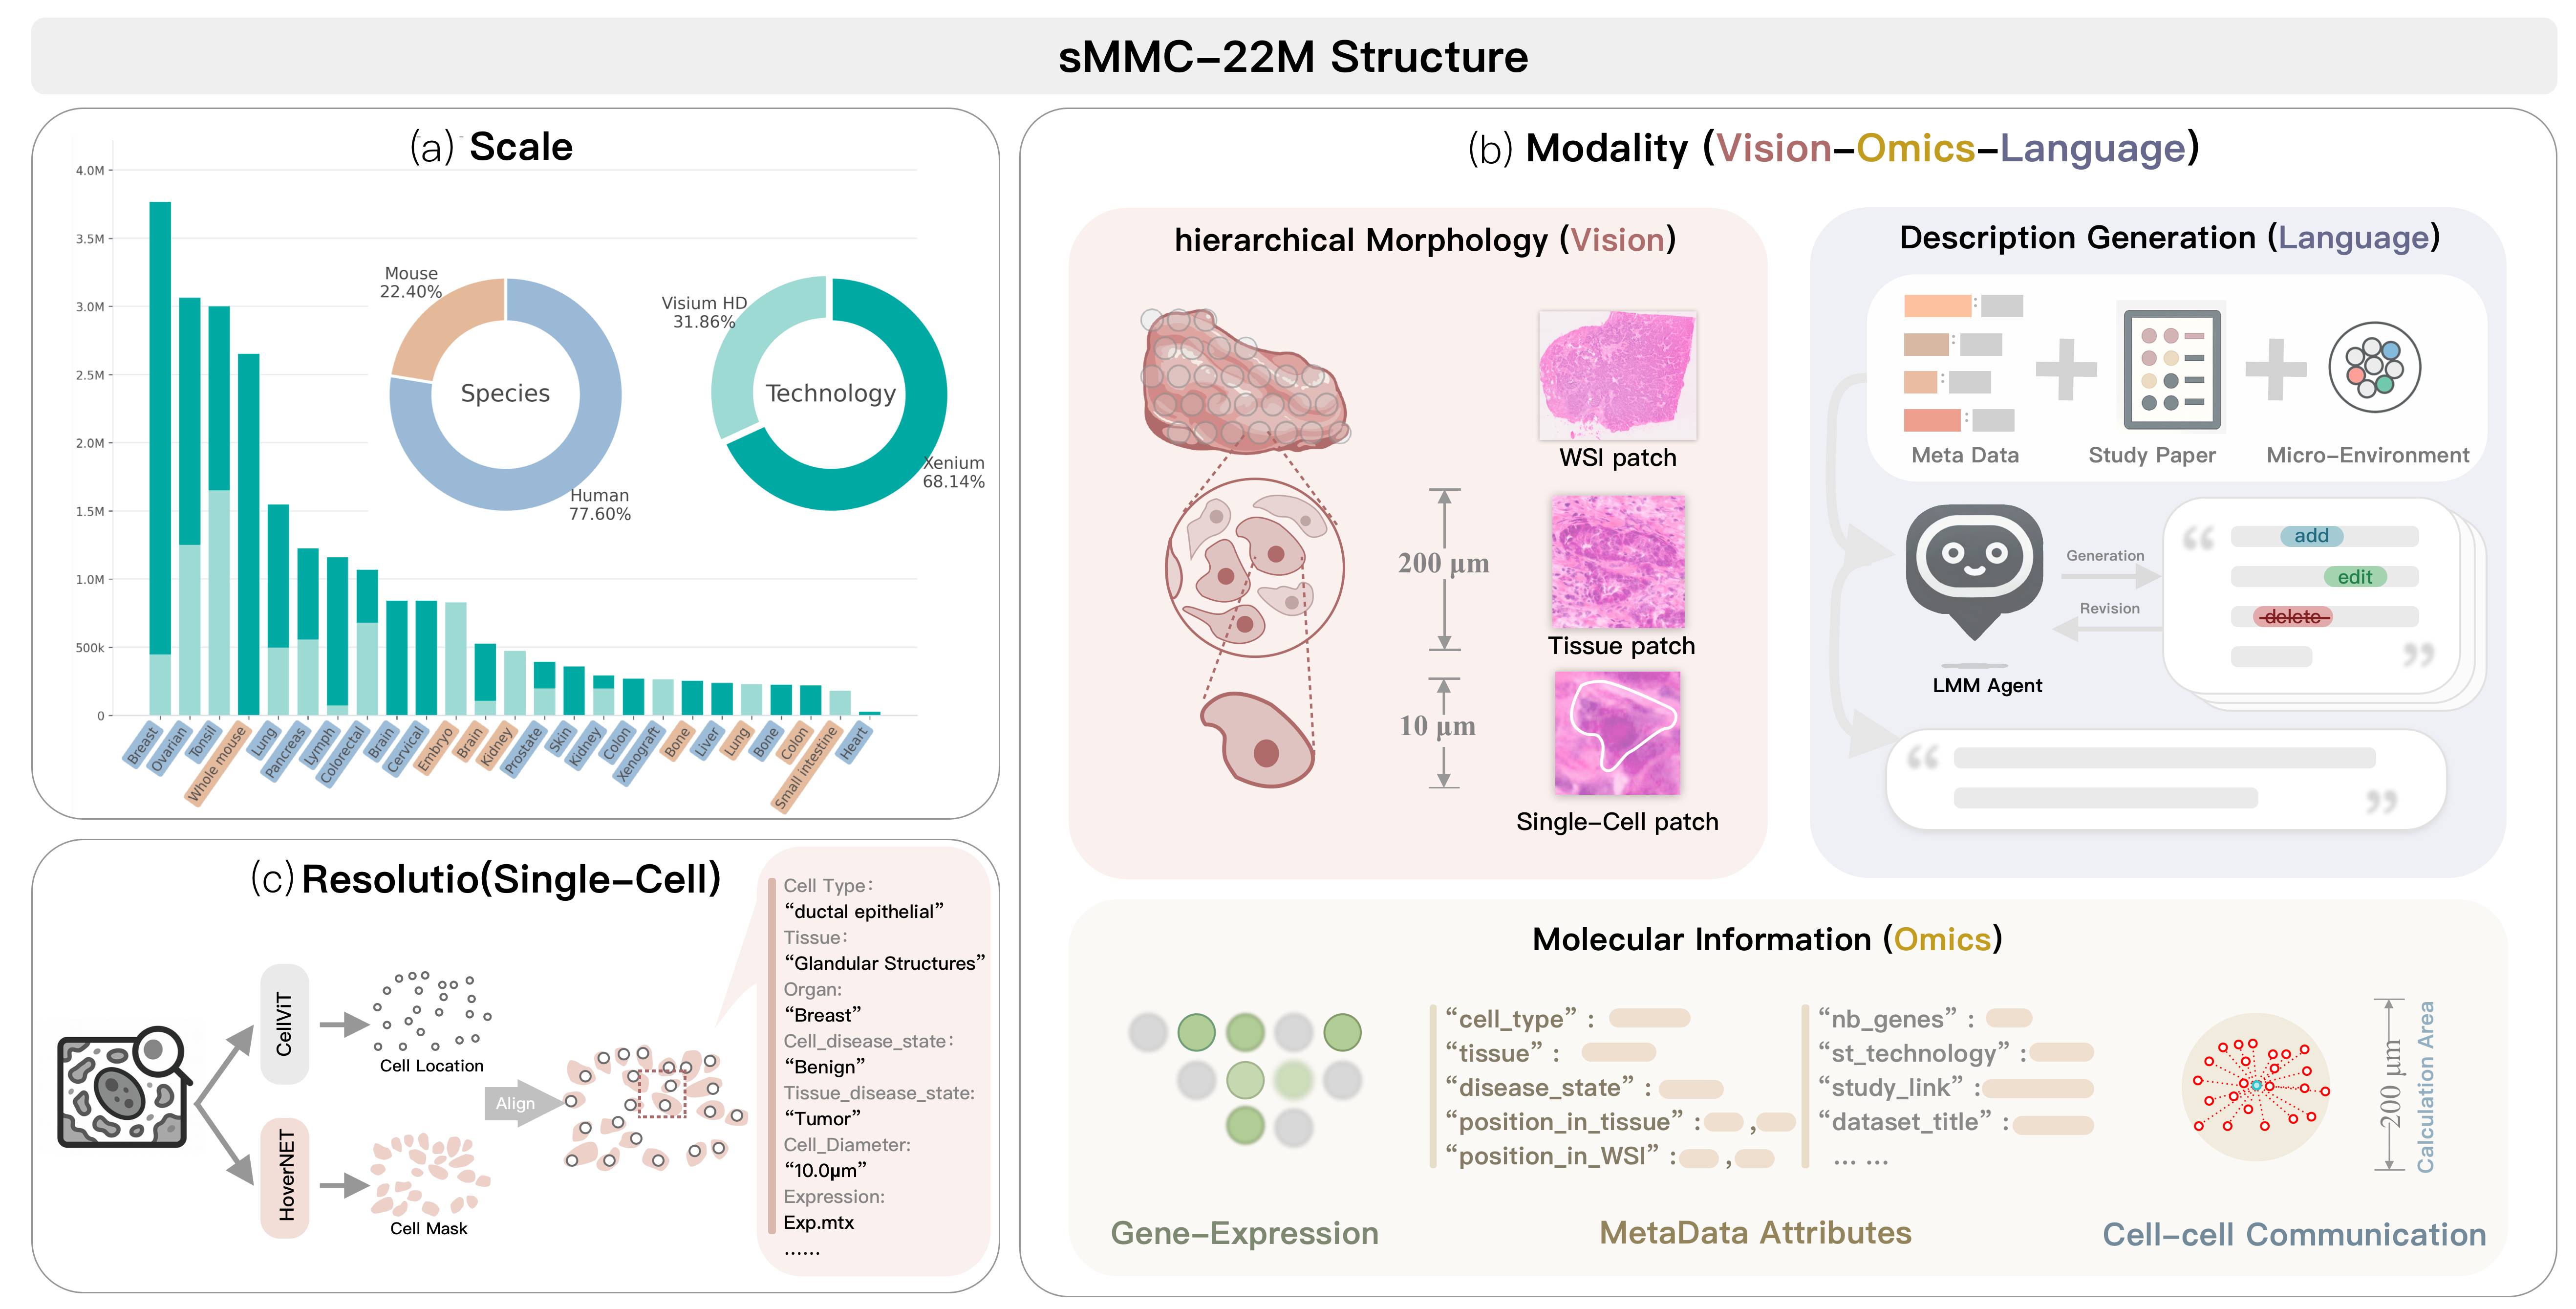
\includegraphics[width=0.98\linewidth]{dataset.png}
    \caption{Overview of \dataset. The figure summarizes the scale of the resource, the multimodal structure of each record, and the single-cell alignment between histology context and molecular measurements.}
    \label{fig:dataset_overview_ed}
\end{figure*}


\section{Introduction}
Spatial transcriptomics (ST) preserves tissue coordinates while measuring gene
expression, allowing histology to be tested as a proxy for molecular state in
situ. H\&E captures cellular morphology, tissue architecture, and
microenvironmental organization at higher spatial resolution. The central
question is whether benchmarks can measure molecular signals in morphology
under realistic biological variation. At cellular resolution, this requires more
than detecting a pooled association: a benchmark must distinguish neighboring
cell states and test whether the association survives changes in patient,
tissue context, and acquisition condition.

Paired H\&E--ST resources such as HEST-1K and STimage-1K4M have advanced this
evaluation~\cite{jaume2025hest,chen2024stimage}, yet three limitations remain.
First, their scale does not capture the diversity of organs, patients, studies,
and acquisition conditions. Second, spot-level targets average multiple cells
and hide cellular heterogeneity. Third, image--expression pairs often lack
biological context such as age, disease, and neighborhood organization.
Consequently, pooled scores may reflect narrow-cohort interpolation rather than
biologically robust prediction. These limitations are coupled: larger
collections without cell alignment preserve spot averaging, while cell-aligned
records without context cannot reveal whether a score is concentrated in one
cohort. A useful benchmark must expose all three dimensions under a common
evaluation interface.

We introduce \dataset, a context-aware resource organized around
\textbf{scale}, \textbf{resolution}, and \textbf{rich context}
(\Cref{fig:dataset_overview_ed}). Its current manifest contains 28{,}315{,}247
aligned targets across 25 tissue categories and 99 unique samples (100 records)
(\Cref{tab:main_release_manifest}). Each benchmark unit is an aligned cell
rather than a mixed spot, and each record links histology, expression, spatial
coordinates, neighborhood information, and sample attributes. Scale supports
controlled comparisons among pathology encoders; resolution separates native
Xenium cells from derived Visium HD cell-aligned targets; and context supports
explicit transfer and worst-context evaluation. The name
\dataset is retained from the frozen release, while the versioned manifest
tracks subsequent public and in-house additions.

\dataset makes three contributions. First, it releases a large cell-aligned ST
resource with matched H\&E, expression, and context. Second, it provides a
data-centric interface for lifting spot-level image-to-gene pipelines to
single-cell prediction. Third, it demonstrates that benchmark behavior depends
on data scale, cellular resolution, and explicit context through encoder
scaling, leakage-controlled transfer, and support-aware audits
(\Cref{fig:encoder_scaling_placeholder,fig:main_exp,tab:breadth_25,tab:context_bias_audit}).
Representative studies appear in the main paper, while construction audits,
platform-transfer support, sensitivity analyses, and downstream diagnostics
are retained in the appendix so that the central claims remain traceable
without conflating native and derived targets.

\section{Related Resources and Benchmarks}

\noindent\textbf{Histology--Omics Resources.}
\dataset builds on three strands of prior work. First, spatial profiling evolved from Spatial Transcriptomics~\cite{stahl2016spatial}, in situ sequencing~\cite{ke2013situ}, MERFISH~\cite{moffitt2016high}, Slide-seq~\cite{rodriques2019slideseq}, and multiplexed imaging~\cite{wang2018multiplexed,eng2019transcriptome} to higher-resolution or higher-throughput platforms such as HDST~\cite{vickovic2019hdst}, Slide-seqV2~\cite{stickels2021slideseqv2}, DBiT-seq~\cite{liu2020dbitseq}, Visium~\cite{10xgenomics2019visium}, high-definition commercial systems~\cite{janesick2023high,oliveira2024characterization}, and spatiotemporal profiling~\cite{chen2022spatiotemporal}. Second, spatial analysis and integration tools, including Giotto~\cite{dries2021giotto}, Squidpy~\cite{palla2022squidpy}, SpaGCN~\cite{hu2021spagcn}, BayesSpace~\cite{zhao2021bayesspace}, Tangram~\cite{biancalani2021deep}, cell2location~\cite{kleshchevnikov2022cell2location}, related cell-type transfer methods~\cite{bergenstrahle2020super,moncada2020integrating,andersson2020single,satija2015spatial}, Impeller~\cite{duan2024impeller}, iMiracle~\cite{duan2024imiracle}, Disco~\cite{duan2025disco}, Muse~\cite{duan2025muse}, Seurat integration~\cite{stuart2019comprehensive,hao2021integrated}, Scanpy~\cite{wolf2018scanpy}, the Human Cell Atlas~\cite{regev2017human}, and Tabula-style resources~\cite{jones2022tabula,rozenblatt2020human}, provide the computational and single-cell reference backbone. Third, HEST-1K~\cite{jaume2025hest} and STimage-1K4M~\cite{chen2024stimage} connect histology--omics pairs with evaluation, whereas \dataset additionally provides cell alignment, multi-organ coverage, transfer splits, and structured context (\Cref{tab:resource_comparison_ed}).

\noindent\textbf{Histology-to-Gene Prediction.}
HE2RNA showed bulk transcriptomic prediction from digital pathology~\cite{pronier2020he2rna}, while Hist2ST~\cite{zeng2022spatial}, BLEEP~\cite{xie2023spatially}, iSTAR~\cite{zhang2024inferring}, and THItoGene~\cite{jia2024thitogene} established spot- or region-level histology-to-gene prediction. These methods are supported by a broader pathology modeling stack: weakly supervised WSI and MIL-style learning~\cite{campanella2019clinical,lu2021data,shao2021transmil,ciga2022self,ilse2018attention}, dense nuclear and cellular modeling~\cite{ronneberger2015unet,graham2019hover,horst2024cellvit}, and studies linking morphology with diagnosis or molecular inference~\cite{bejnordi2017diagnostic,wang2016deep,komura2018machine,kather2019deep}. Our benchmark differs by targeting cell-aligned image-to-gene prediction rather than bulk, slide-level, or spot-averaged prediction, under controlled in-domain and transfer splits.

\noindent\textbf{Pathology Foundation Models and Multimodal Learning.}
Large pathology encoders define this benchmark's representation-learning context. Representative models include QuiltNet~\cite{ikezogwo2023quilt1m}, pathology transformers~\cite{wang2022transformer}, robust pathology pretraining~\cite{azizi2023robust}, UNI and UNI2-h~\cite{chen2024uni,mahmoodlab_uni2h}, Phikon~\cite{filiot2024phikon}, GigaPath~\cite{xu2024whole}, Virchow~\cite{vorontsov2023virchow}, Virchow2~\cite{zimmermann2024virchow2}, H-optimus-0~\cite{hoptimus0}, CONCH~\cite{lu2024visual}, PLIP~\cite{huang2023visual}, PathCLIP~\cite{he2024pathclip}, BiomedCLIP~\cite{zhang2023biomedclip}, and PathGen-style corpora~\cite{sun2024pathgen}. They also build on visual corpora and CNN or transformer backbones, including EfficientNetB0/EfficientNet~\cite{deng2009imagenet,lin2014microsoft,he2016deep,koonce2021resnet,simonyan2015very,szegedy2015going,tan2019efficientnet,dosovitskiy2021image,touvron2021training,liu2021swin,liu2022convnet}, self-supervised and masked objectives~\cite{he2020momentum,chen2020simple,grill2020bootstrap,zbontar2021barlow,caron2018deep,caron2020unsupervised,chen2021exploring,caron2021emerging,oquab2023dinov2,he2022masked,baevski2022data2vec}, and multimodal or language foundation models~\cite{radford2021learning,devlin2019bert,raffel2020exploring,achiam2023gpt4,bommasani2021opportunities,koh2021wilds}. For cellular context and out-of-domain evaluation, it also relates to nuclei-level resources such as PanNuke~\cite{gamper2020pannuke} and public cancer pathology cohorts such as TCGA~\cite{weinstein2013cancer}. Separately, the main evaluation uses two public 10x Visium HD human lung cancer examples as A/B within-assay sources~\cite{tenx_visium_hd_postx_lung_ffpe,tenx_visium_hd_lung_fixed_frozen}. Here, these works serve as background: text annotations provide auxiliary context for future multimodal evaluation, not the primary prediction target.







\begin{table}[t]
\centering
\footnotesize
\setlength{\tabcolsep}{2.2pt}
\renewcommand{\arraystretch}{1.10}
\caption{\textbf{Resource comparison.} Coverage is reported directly as
Yes, No, or Partial. Row groups indicate each resource's primary intent.}
\label{tab:resource_comparison_ed}
\begin{tabularx}{\columnwidth}{@{}
>{\raggedright\arraybackslash}X
>{\centering\arraybackslash}m{0.72cm}
>{\centering\arraybackslash}m{0.84cm}
>{\centering\arraybackslash}m{0.84cm}
>{\centering\arraybackslash}m{1.25cm}
>{\centering\arraybackslash}m{1.05cm}
@{}}
\toprule
\textbf{Resource} &
\shortstack{\textbf{Cell}\\\textbf{level}} &
\shortstack{\textbf{Multi}\\\textbf{organ}} &
\shortstack{\textbf{Study}\\\textbf{split}} &
\shortstack{\textbf{Platform}\\\textbf{transfer}} &
\shortstack{\textbf{Text /}\\\textbf{context}} \\
\midrule
\rowcolor[gray]{0.94}
\multicolumn{6}{l}{\textit{Single-cell-only atlas}} \\
CELLxGENE Census & Yes & Yes & Yes & No & No \\
\addlinespace[2pt]
\rowcolor[gray]{0.94}
\multicolumn{6}{l}{\textit{Pathology image--text corpora}} \\
OpenPath & No & Partial & No & No & Yes \\
Quilt-1M & No & Partial & No & No & Yes \\
PathGen-1.6M & No & Partial & No & No & Yes \\
\addlinespace[2pt]
\rowcolor[gray]{0.94}
\multicolumn{6}{l}{\textit{ST + histology resources}} \\
HEST-1K & No & Yes & Yes & Partial & No \\
STimage-1K4M & No & Yes & Partial & Partial & No \\
\addlinespace[2pt]
\rowcolor[rgb]{0.90,0.95,1.00}
\textbf{\dataset} & Yes & Yes & Yes & Yes & Partial \\
\bottomrule
\end{tabularx}
\end{table}

\section{The \dataset Resource}
\subsection{Design Objectives}
\dataset is organized around three design requirements. First, it supports
cell-aligned rather than only spot-level evaluation. Second, it preserves
spatial context around each cell instead of reducing a record to an isolated
molecular profile or a few image patches. Third, it spans sufficient organ,
study, and species diversity for reproducible benchmark splits rather than
only large-scale pretraining (\Cref{fig:dataset_overview_ed}).

\subsection{Scale, Coverage, and Sources}
We describe \dataset through the same three axes used throughout the paper:
\textbf{scale}, \textbf{resolution}, and \textbf{rich context information}.
These axes motivate the experiments, but their interpretation depends on how
the resource is constructed.

\paragraph{Scale.}
\dataset combines public Xenium and Visium HD experiments with new in-house
DBiC-seq data. The current manifest contains 28{,}315{,}247 aligned targets
from 99 unique samples (100 versioned records), spanning 25 tissue categories
and three cell-line origins (\Cref{tab:main_release_manifest}). This breadth
enables evaluation across samples, biological contexts, and acquisition
settings rather than only within a narrow in-domain setting. It also allows
organ-macro reporting, so large lung or tonsil samples cannot dominate results
from smaller categories. The frozen release has a long-tailed composition, and
platform-transfer support varies by organ
(\Cref{fig:dataset_scale,tab:all_xenium_visium_summary}).

\paragraph{Resolution.}
The resource is organized around cell-aligned targets rather than only mixed
spots. Each example is anchored to a specific cell and its tissue coordinates,
preserving spatial provenance instead of collapsing neighboring cells into a
regional average. This organization supports leakage-controlled splits,
record-level tracing to study, sample, organ, platform, and coordinate system,
and separation of local interpolation from transfer across slides or cohorts.
Xenium supplies native segmented cells, whereas Visium HD targets are derived
through bin-to-cell aggregation (\Cref{fig:bin2cell}).

\paragraph{Rich modality and context information.}
Each cell is represented as a multimodal record rather than an image crop
alone. Its core representation combines hierarchical histology context, a
cell-level expression profile, and structured metadata, with optional spatial
descriptors for neighborhood organization and cell--cell communication.
Together, these channels support analyses in which morphology, molecular
state, sample attributes, and local tissue context must be studied jointly
(\Cref{tab:data_schema}). Structured fields remain the primary source of
benchmark labels; generated captions and communication summaries are optional
derived artifacts rather than required supervision.

\begin{table*}[!t]
\centering
\footnotesize
\setlength{\tabcolsep}{2.4pt}
\renewcommand{\arraystretch}{1.04}
\setlength{\abovecaptionskip}{4pt}
\setlength{\belowcaptionskip}{3pt}

\caption{\textbf{Release interface and benchmark coverage.}
Counts are aligned targets after QC. The light-blue row marks the new in-house
primary data included in the current working manifest.}
\label{tab:main_release_manifest}

\begin{tabularx}{\textwidth}{
>{\raggedright\arraybackslash}p{2.25cm}
>{\raggedright\arraybackslash}p{1.35cm}
>{\raggedright\arraybackslash}p{2.15cm}
>{\raggedright\arraybackslash}p{1.65cm}
>{\raggedright\arraybackslash}p{1.75cm}
>{\raggedleft\arraybackslash}p{1.45cm}
>{\raggedright\arraybackslash}X
}
\toprule
\textbf{Block} &
\textbf{Samples} &
\textbf{Scope} &
\textbf{Platform} &
\textbf{Cell / target unit} &
\textbf{Targets} &
\textbf{Coverage or release note} \\
\midrule
\rowcolor{gray!12}
\multicolumn{7}{l}{\textit{Release interface and benchmark coverage}} \\
Expanded manifest &
99 unique (100 records) &
25 tissue categories + 3 cell-line origins &
Xenium; Visium HD; DBiC-seq &
Native / derived aligned target &
28{,}315{,}247 &
In-domain, cross-sample, cross-platform, and context-shift evaluation \\
Xenium source block &
42 &
human and mouse tissues &
Xenium &
Native segmented cell &
16.31M &
In-domain and cross-platform single-cell evaluation \\
Visium HD source block &
36 &
human, mouse, and other species &
Visium HD &
Derived bin-to-cell target &
11.95M &
In-domain, cross-sample, and cross-platform evaluation \\
\rowcolor{inhouseblue}
New in-house primary data &
21 &
mouse-embryo; cervical; lung &
DBiC-seq &
Native cell &
53{,}989 &
In-domain/context-aware; 54{,}304 measured and 315 removed by QC \\
Reviewer subset &
sub. &
review records &
Mixed &
Cell-aligned &
rec. &
Smoke testing and lightweight figure/table regeneration \\
Benchmark package &
-- &
all supported categories &
Mixed &
Split-indexed &
fixed &
In-domain for all categories; transfer protocols where supported \\
\bottomrule
\end{tabularx}

\vspace{1pt}
{\scriptsize\emph{Notes:} ``sub.'' and ``rec.'' denote subset- and
record-level derived artifacts. One versioned breast slide explains 99 unique
samples versus 100 records. Anonymous release:
\url{https://anonymous.4open.science/r/sMMC-22M-DB75}.}
\end{table*}

Gene targets are omitted from the table for readability: Xenium uses panel
genes, Visium HD uses processed full-transcriptome targets, and cross-platform
experiments use harmonized shared genes. Full per-sample gene counts, source
identifiers, QC status, benchmark-coverage fields, and checksum-backed paths
are provided in the released CSV.

The overview distinguishes native and derived target units and highlights the
new in-house contribution (\Cref{tab:main_release_manifest}). The mutually
exclusive provenance partition is reported in the appendix
(Appendix~\Cref{tab:appendix_provenance_audit}). In the complete manifest, each
source sample is linked to its platform, organ, cell count, gene target,
upstream source, license note, inclusion status, and QC outcome.
This distinction prevents aggregated public data, newly measured in-house
cells, and processed derivatives from being counted as equivalent forms of
novel data.



\subsection{Cell-Aligned Multimodal Structure}

Each record is defined around one segmented or platform-defined cell rather
than a spot, tile, or slide region. It links multiscale histology crops centered
on that cell with a molecular target, spatial coordinates, sample and platform
metadata, and optional neighborhood or cell--cell communication descriptors.
This cellular anchor allows image, omics, and context features to be evaluated
at the same biological unit. It also keeps the image crop, expression target,
split assignment, and sample metadata joined by one stable identifier, which
reduces ambiguity during downstream evaluation.

The design changes the benchmark question from recovering expression averaged
over a mixed local region to predicting fine-grained molecular variation from
cell morphology and local tissue context. The same schema supplies the
input--target format through which STBoost lifts spot-level image-to-gene
pipelines to cell-aligned prediction.

\subsection{Alignment Pipeline}
The alignment pipeline is auditable end to end. We first localize the assayed
tissue region, define cell locations through segmentation or platform masks,
and then extract matched image context and molecular measurements. Because
errors can compound across stages, each stage is tracked explicitly. For
Visium HD, dense expression bins are assigned to segmented H\&E cell footprints
and aggregated with boundary-aware quality control. For Xenium,
platform-provided boundaries and transcript coordinates define the native
cell unit. Each record therefore retains slide provenance, a segmented or
platform-defined footprint, aligned molecular counts, and multiscale histology
centered on the same cell (\Cref{fig:bin2cell,tab:data_schema}).


% \subsection{Limitations of the Resource}
%Although \dataset is large, it is not biologically uniform. Organ frequencies are imbalanced, some diseases and platforms are overrepresented, and only a subset of organs support the strongest cross-study or cross-slide evaluation regimes. In addition, textual annotations are metadata-grounded rather than independently curated biological descriptions, and should therefore be interpreted as auxiliary context rather than as error-free labels. These limitations do not diminish the value of the resource, but they do constrain the claims that can reasonably be made from benchmark results.

%\section{The \benchmarkname Benchmark}
%\subsection{Benchmark Scope}
%\benchmarkname is intended to measure how well histology-based systems predict molecular state under increasingly realistic evaluation regimes. Rather than reporting only a single overall score, the benchmark separates local interpolation from transfer across slides, studies, organs, and technologies.


\section{How \dataset Boosts Existing ST Research}
\subsection{Scale: Large Coverage Enables Encoder Scaling Laws}
Scale is not only a pretraining convenience; it changes what can be measured.
Broad coverage lets us test whether model capacity and pretraining breadth
improve morphology--gene correspondence under a fixed cell-aligned interface
rather than across unrelated preprocessing pipelines.

The manifest supports controlled encoder evaluation under a fixed cell-level
interface (28{,}315{,}247 targets, 25 categories, 99 unique samples/100
records, and 21 in-house samples; \Cref{tab:main_release_manifest}). The full
inventory and long-tail composition are reported in the appendix
(\Cref{fig:dataset_scale,tab:all_xenium_visium_summary,tab:organ_gene_cell_coverage}).
The two encoder tasks below are representative scaling tests rather than a
claim of exhaustive organ coverage; the organ-wide analysis is reported
separately.

Following the HEST-1K protocol~\cite{jaume2025hest}, we evaluated seven
histopathology encoders under a unified frozen-embedding retrieval and
prediction framework on mouse brain and human lung cancer. Pathology-pretrained
encoders outperformed generic backbones. H-Optimus-0 led average Pearson on
both tasks, while UNI led brain sensitivity and accuracy; H-Optimus-0 led both
measures on lung
(average Pearson: 0.567 brain and 0.449 lung; sensitivity/accuracy: UNI
0.807/0.697 on brain and H-Optimus-0 0.643/0.623 on lung;
\Cref{fig:encoder_scaling_placeholder}a). Thus, pathology pretraining improved
morphology-derived representations under matched evaluation.

We then used frozen encoder embeddings to predict the top 50 highly variable
genes within patient. Additional in-domain training consistently improved
prediction
(training ratio 0.05 to 0.25; \Cref{fig:encoder_scaling_placeholder}b).
H-Optimus-0, UNI2-h, and UNI formed the leading group, showing that the scale
increase adds usable morphology--gene signal rather than only records.

Performance also improved broadly with encoder capacity and pathology
pretraining: ResNet50, CTransPath, and Phikon formed the lower tier, CONCH was
intermediate, and UNI, UNI2-h, and H-Optimus-0 led
(\Cref{fig:encoder_scaling_placeholder}c). These analyses support frozen
pathology foundation models as useful baselines for cell-aligned
morphology--gene benchmarking. Protocol details and stable retrieval tables
are provided in Appendix~\Cref{sec:benchmark_protocol}.

\begin{figure*}[t]
\centering
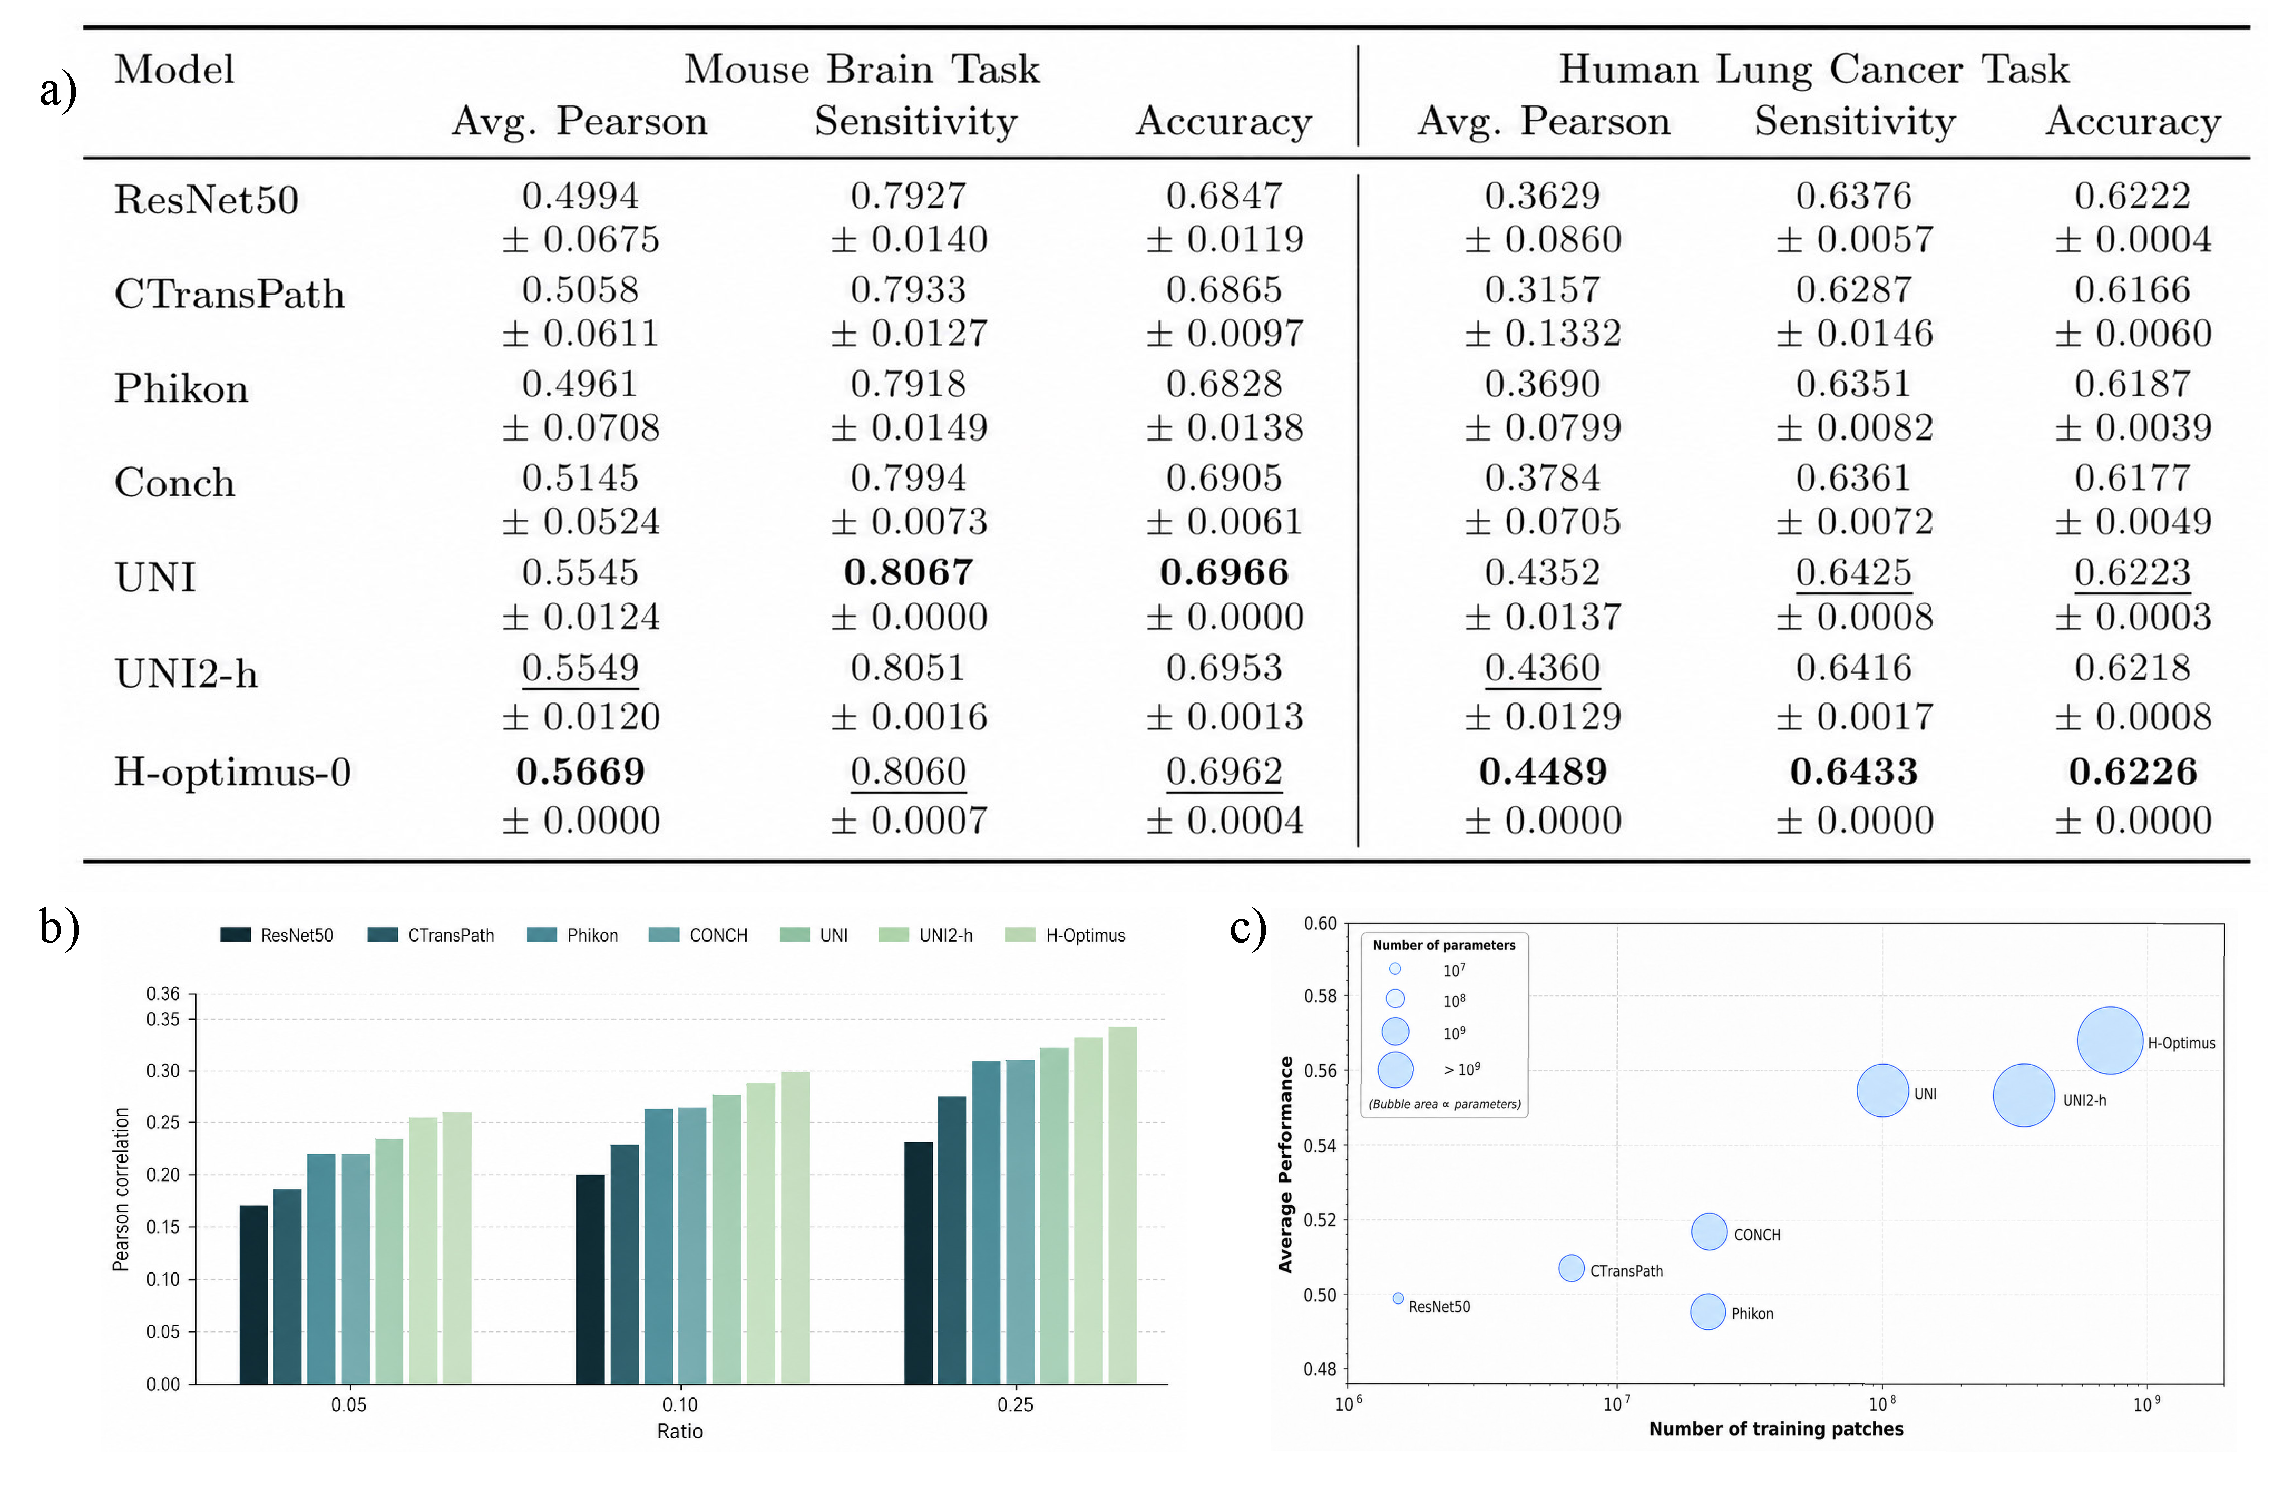
\includegraphics[width=0.9\linewidth]{benchmark.pdf}
\caption{\textbf{Encoder benchmarking and scaling behavior on sMMC-22M.}
(a) Seven pathology encoders are evaluated on mouse brain and human lung cancer; H-Optimus-0 leads average Pearson, while UNI leads mouse-brain sensitivity and accuracy.
(b) In-patient prediction of the top 50 variable genes improves with training size, with H-Optimus-0 strongest across ratios.
(c) Scaling analysis shows that larger models and broader pretraining improve performance, with UNI, UNI2-h, and H-Optimus-0 forming the leading tier.}
\label{fig:encoder_scaling_placeholder}
\end{figure*}

\noindent\textbf{Biological calibration.}
Whole-panel correlation can be difficult to interpret biologically, so we also
evaluated training-selected marker/HVG overlap and cell-type-stratified
pseudobulk profiles. Marker selection used only the training partition, while
pseudobulk profiles aggregated predictions within expression-derived coarse
cell states. These views test whether a whole-panel score retains interpretable
gene and cell-state structure.
Image features retained substantially more marker-level signal and aggregate
cell-state structure than coordinate-only, spatial-KNN, or training-mean
controls across 30 native-Xenium samples (marker/HVG Gene Pearson: 0.201
versus 0.031, 0.028, and 0.000; cell-type pseudobulk RMSE: 0.120 versus
0.224, 0.187, and 0.188; Appendix~\Cref{tab:appendix_biological_calibration}).
Because cell-type labels are expression-derived, this is aggregate calibration
rather than independent cell-type validation.

\noindent\textbf{STBoost breadth beyond the representative cases.}
We next evaluated \methodname across all 25 release categories. Genes were
selected from the training partition only, and every category used the same
spatially buffered evaluation design. \methodname led Gene Pearson in 21 of 25
categories under training-only gene selection, four contiguous spatial edge
holdouts, and a 5\% coordinate-span buffer (\Cref{tab:breadth_25}). Bone,
Liver, Plant, and Seed remained explicit failure cases. Across 30 native-Xenium
samples, \methodname reached a Gene Pearson of 0.324 versus 0.046 for
coordinate-only and 0.053 for spatial KNN
(sample-bootstrap 95\% CI 0.277--0.368; \Cref{tab:breadth_25}). This
organ-macro result extends the scale claim beyond the two representative
tissues.
Reporting each category separately avoids a cell-weighted pooled average in
which large samples could mask failure on long-tail organs and non-human
categories.

\begin{table}[t]
\centering
\scriptsize
\setlength{\tabcolsep}{0.5pt}
\renewcommand{\arraystretch}{0.98}
\caption{\textbf{STBoost cell-aligned results across all 25 release
categories.}
Categories are grouped by species; mixed-species and other-organism categories
are listed separately. Bold entries in the three Gene-Pearson columns mark the
best of \methodname, coordinate-only, and spatial-KNN predictions.}
\label{tab:breadth_25}
\label{tab:breadth_25a}
\label{tab:breadth_25b}
\begin{tabular*}{\columnwidth}{@{\extracolsep{\fill}}lrrrrrr@{}}
\toprule
& \multicolumn{3}{c}{\scriptsize Gene Pearson}
& \multicolumn{3}{c}{\scriptsize STBoost prediction} \\
\cmidrule(lr){2-4}\cmidrule(lr){5-7}
Category &
{\scriptsize STBoost} &
{\scriptsize\shortstack{Coordinate\\only}} &
{\scriptsize\shortstack{Spatial\\KNN}} &
{\scriptsize\shortstack{Gene\\Spearman}} &
{\scriptsize\shortstack{Cell\\Pearson}} &
{\scriptsize F1} \\
\midrule
\rowcolor{gray!18}\multicolumn{7}{@{}l}{\textbf{Mouse organs}} \\
Bone & 0.030 & \textbf{0.124} & 0.055 & 0.037 & 0.180 & 0.240 \\
Colon & \textbf{0.615} & -0.137 & 0.072 & 0.588 & 0.739 & 0.744 \\
Embryo & \textbf{0.278} & 0.037 & 0.045 & 0.251 & 0.517 & 0.342 \\
Small intestine & \textbf{0.572} & -0.104 & 0.067 & 0.548 & 0.701 & 0.715 \\
\addlinespace[2pt]
\rowcolor{gray!18}\multicolumn{7}{@{}l}{\textbf{Human organs}} \\
Breast & \textbf{0.400} & 0.053 & 0.035 & 0.375 & 0.433 & 0.487 \\
Cervical & \textbf{0.178} & 0.017 & 0.014 & 0.157 & 0.247 & 0.026 \\
Colorectal & \textbf{0.431} & 0.056 & 0.083 & 0.419 & 0.532 & 0.623 \\
Heart & \textbf{0.292} & 0.010 & 0.021 & 0.266 & 0.688 & 0.304 \\
Kidney & \textbf{0.402} & 0.019 & 0.017 & 0.361 & 0.471 & 0.460 \\
Liver & -0.002 & 0.003 & \textbf{0.010} & -0.002 & 0.561 & 0.400 \\
Lung & \textbf{0.359} & 0.065 & 0.053 & 0.317 & 0.402 & 0.457 \\
Lymph node & \textbf{0.141} & 0.043 & 0.013 & 0.131 & 0.164 & 0.023 \\
Ovarian & \textbf{0.250} & 0.122 & 0.104 & 0.239 & 0.312 & 0.234 \\
Ovarian glands & \textbf{0.402} & 0.059 & 0.043 & 0.391 & 0.559 & 0.756 \\
Pancreas & \textbf{0.324} & 0.090 & 0.068 & 0.272 & 0.505 & 0.275 \\
Pancreatic & \textbf{0.366} & 0.080 & 0.051 & 0.341 & 0.540 & 0.694 \\
\shortstack[l]{Pancreatic duct\\gland} & \textbf{0.331} & 0.091 & 0.100 & 0.282 & 0.408 & 0.386 \\
Prostate & \textbf{0.263} & -0.015 & 0.025 & 0.244 & 0.263 & 0.083 \\
Skin & \textbf{0.359} & 0.048 & 0.086 & 0.299 & 0.437 & 0.368 \\
Tonsil & \textbf{0.294} & 0.028 & 0.018 & 0.249 & 0.462 & 0.399 \\
\addlinespace[2pt]
\rowcolor{gray!18}\multicolumn{7}{@{}l}{\textbf{Mixed and other species}} \\
\shortstack[l]{Brain(Human+Mouse)} & \textbf{0.399} & 0.010 & 0.036 & 0.371 & 0.570 & 0.752 \\
Head (zebrafish) & \textbf{0.216} & 0.022 & 0.031 & 0.193 & 0.429 & 0.287 \\
Plant (\textit{A. thaliana}) & -0.011 & 0.004 & \textbf{0.012} & -0.009 & 0.385 & 0.052 \\
Seed (soybean) & -0.020 & -0.003 & \textbf{0.008} & -0.018 & 0.314 & 0.037 \\
\shortstack[l]{Xenograft} & \textbf{0.387} & 0.041 & 0.049 & 0.362 & 0.526 & 0.589 \\
\midrule
\textbf{30-sample macro} & \textbf{0.324} & 0.046 & 0.053 &
\textbf{0.291} & \textbf{0.442} & \textbf{0.413} \\
\bottomrule
\end{tabular*}
\end{table}

\subsection{Resolution: From Spot-Level Prediction to Single-Cell Prediction}
Most public histology-to-gene resources and baselines are organized around
mixed ST spots. This setting is useful for regional prediction, but it can
conflate cells with different states inside one measured area. \dataset instead
defines an aligned cell as the benchmark unit. Every record contains a cell
footprint, cell-centered and contextual histology crops, spatial coordinates,
and a molecular target. Visium HD records aggregate dense 2\,$\mu$m bins within
segmented footprints with boundary-aware quality control, whereas Xenium
records use platform-defined boundaries and transcript coordinates
(Appendix~\ref{sec:st}; \Cref{fig:bin2cell}).

\noindent\textbf{STBoost framework.}
STBoost is a model-agnostic interface that converts spot-level
histology--omics predictors into single-cell predictors. A method need not
change its high-level learning objective; STBoost instead changes the
input--target interface. It replaces spot-centered image crops and
spot-averaged expression with aligned cell footprints, cell-centered crops,
larger contextual crops, coordinates, and cell-level molecular targets.
Existing BLEEP, Hist2ST, and HisToGene-style pipelines can therefore retain
their learning objectives while operating on a shared cell-aligned format
(\Cref{fig:architecture_framework}, left).
STBoost is therefore a data-centric conversion framework, not a claim that one
new architecture supersedes every spot-level method.

Our BLEEP instantiation trains the original image--expression alignment model
on the records produced by STBoost, yielding STBoosted BLEEP
(\Cref{fig:architecture_framework}, right). This instantiation tests whether a
representative spot-level model can be lifted under the same
leakage-controlled splits. We compare it with the native single-cell
STBoost-Ref baseline on matched cells and shared genes
(\Cref{fig:main_exp}). STBoost-Ref architecture details are provided in
Appendix~\ref{sec:STBoost_appendix_details}.

\begin{figure*}[t]
\centering
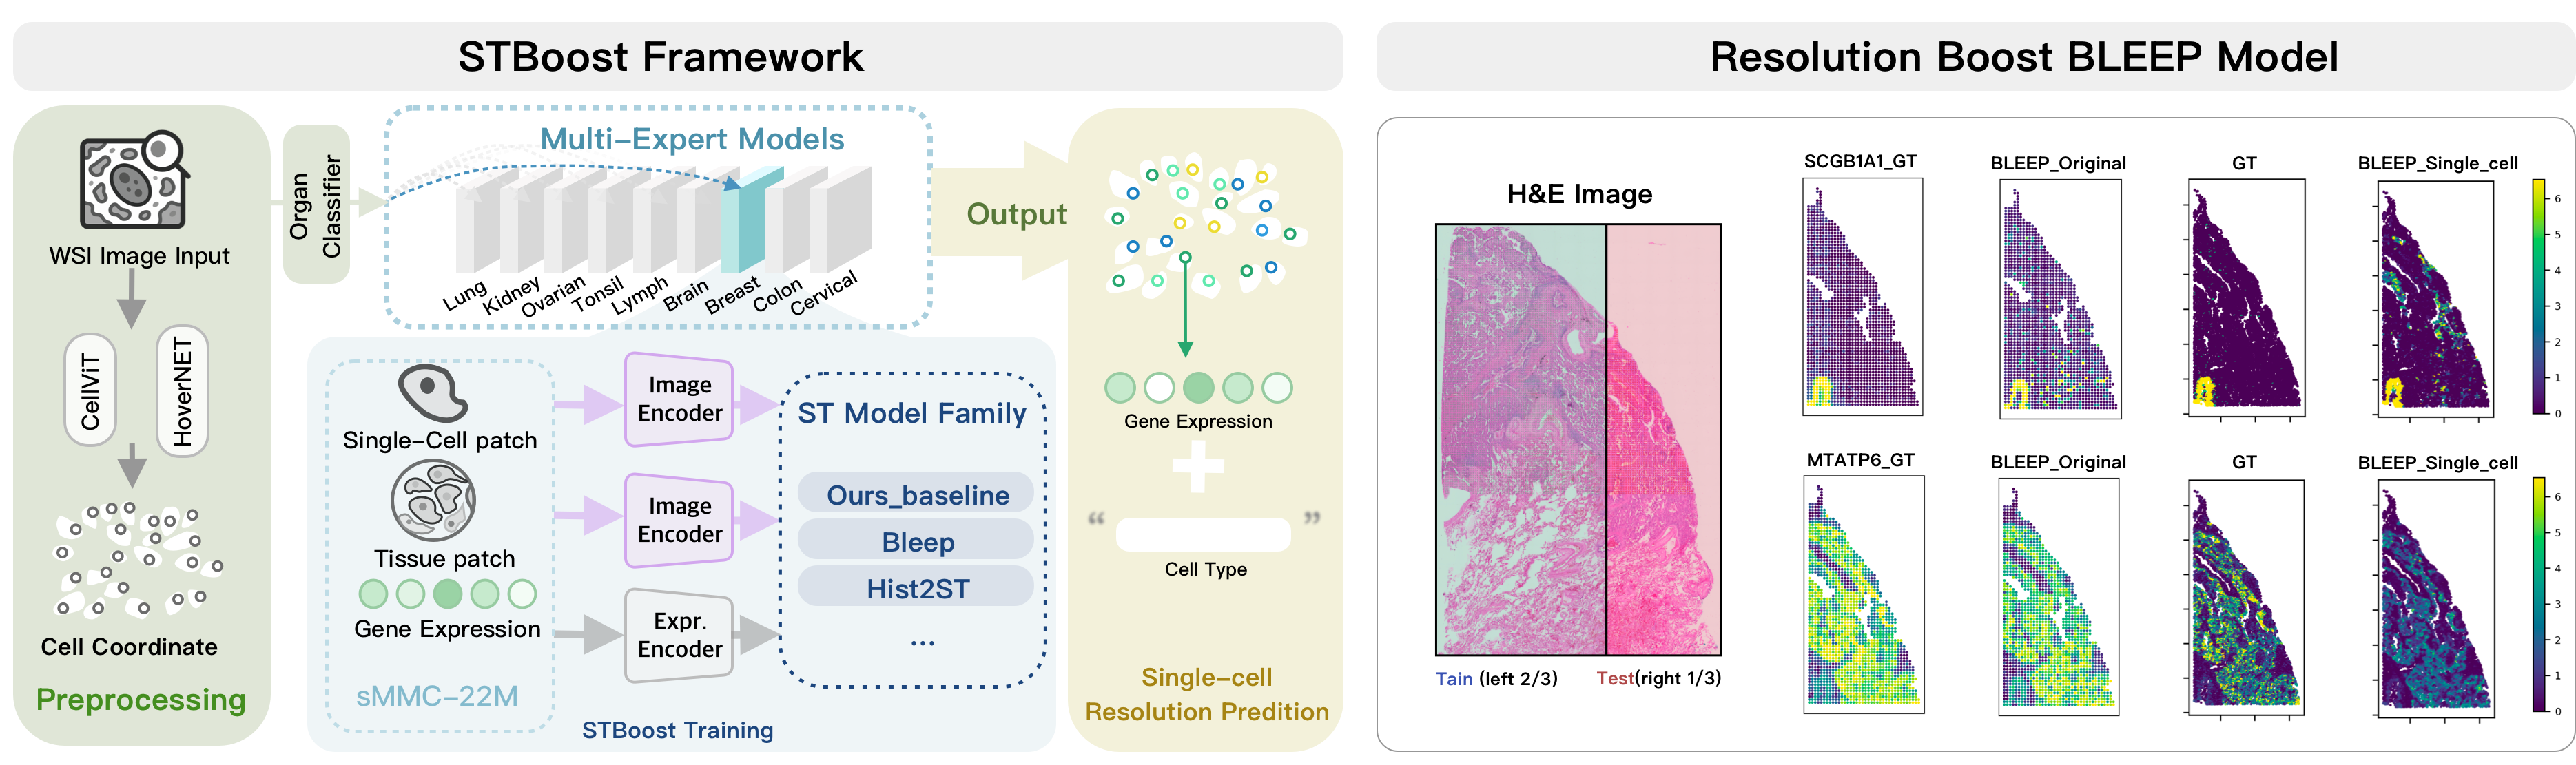
\includegraphics[width=0.98\linewidth]{STBoost.png}
\caption{\textbf{STBoost converts spot-level histology--omics models into single-cell predictors.} Left: STBoost forms aligned cell-level records from cell footprints, cell-centered/contextual histology crops, spatial coordinates, and matched molecular targets, enabling spot- or patch-based pipelines to operate at single-cell resolution. Right: a BLEEP instantiation replaces spot crops and targets with this cell-aligned interface, yielding STBoosted BLEEP for single-cell image-to-gene prediction.}
\label{fig:architecture_framework}
\end{figure*}


\begin{figure*}[t]
\centering
\includegraphics[width=0.98\linewidth]{main_exp.png}
\caption{\textbf{Single-cell image-to-gene prediction results for STBoost-Ref and BLEEP under our framework.} Both methods are recomputed on the same 5{,}000 test cells and 18{,}085 shared genes per regime (seed 42). Our Baseline model dominates the cross-patient $A\!\to\!B$ setting across F1, correlation, and MSE, and improves most continuous metrics in the in-domain $A\!\to\!A$ setting, while BLEEP retains a marginal F1 advantage on $A\!\to\!A$.}
\label{fig:main_exp}
\end{figure*}


\noindent\textbf{Evaluation protocol.}
The task is image-to-single-cell gene-expression prediction under two
leakage-controlled regimes: \textbf{in-domain} and \textbf{cross-patient}. We
rename two 10x Visium HD human lung cancer examples as A and B:
\begin{itemize}[leftmargin=1.4em,itemsep=0pt,topsep=2pt,parsep=0pt]
    \item \textbf{A}: the Visium HD Spatial Gene Expression Libraries, Post-Xenium, Human Lung Cancer (FFPE) example, analyzed with Space Ranger 3.0.0 \cite{tenx_visium_hd_postx_lung_ffpe}.
    \item \textbf{B}: the Visium HD Spatial Gene Expression Library, Human Lung Cancer (Fixed Frozen) example, analyzed with Space Ranger 3.1.1 \cite{tenx_visium_hd_lung_fixed_frozen}.
\end{itemize}
The in-domain regime trains on the left two thirds of A and tests on the held-out
right third. Cross-patient evaluation retains the A training/validation split
but tests on all cells from B. This separates local interpolation from transfer
to another patient and processing condition. Both methods use the same 5{,}000
test cells, 18{,}085 shared genes, and seed 42 per regime
(\Cref{fig:main_exp}). We report F1, gene-wise and cell-wise
Pearson/Spearman/MSE, and sparsity calibration. Full split definitions, target
details, and additional transfer stress tests are retained in
Appendix~\ref{sec:benchmark_protocol}.
The public names and processing versions are stated explicitly so that A and B
remain reproducible aliases rather than opaque internal sample codes.


\noindent\textbf{In-domain results.}
STBoost-Ref preserved stronger continuous correspondence than BLEEP in-domain,
although BLEEP retained a marginal F1 advantage (F1: 0.1057 versus 0.1065;
gene Pearson/Spearman: 0.0259/0.0268 versus 0.0247/0.0255; cell
Pearson/Spearman: 0.4112/0.1160 versus 0.3458/0.1114; mean MSE: 0.0717 versus
0.0791; \Cref{fig:main_exp}). Thus, a spot-level method can operate on
cell-aligned records, while the native reference better preserves continuous
signal. The comparison does not imply that either method has solved
single-cell expression prediction; it establishes a matched starting point for
cell-aligned model development.
This distinction matters because sparse-gene F1 and continuous correlation
measure complementary aspects of the target rather than interchangeable forms
of accuracy.

\noindent\textbf{Cross-patient results.}
STBoost-Ref outperformed BLEEP on every reported cross-patient metric (F1:
0.1061 versus 0.0857; gene Pearson/Spearman: 0.0124/0.0137 versus
0.0106/0.0117; cell Pearson: 0.2820 versus 0.0896; mean MSE: 0.1504 versus
0.1663; \Cref{fig:main_exp}). It retained 47.9\% of in-domain gene Pearson and
68.6\% of cell Pearson, compared with 42.9\% and 25.9\% for BLEEP
(\Cref{fig:main_exp}). The transferred regime therefore gives STBoost-Ref
1.24$\times$ higher F1 and 3.15$\times$ higher cell Pearson. More importantly,
the retention comparison shows that its advantage is largest under patient
shift rather than local interpolation.
The low gene-wise correlations still caution against interpreting these
predictions as complete molecular reconstructions.

\noindent\textbf{Target-construction sensitivity.}
The native-Xenium evidence above is separated from the Visium HD-derived
targets used in the A/B experiment. We audited 3{,}000 raw segmentation
polygons in each of human lung, mouse brain, and human pancreas
(\(n=9{,}000\)). Expression direction remained stable under one-\(\mu\)m
registration shifts, while bin membership and UMI totals changed measurably
(median cosine 0.936--0.994; \Cref{tab:main_hd_sensitivity}). Unsupported polygons are
removed before release. Erosion/dilation and complete per-sample statistics are
reported in Appendix~\ref{sec:reviewer_validation}. We therefore treat Visium
HD profiles as derived cell-aligned targets rather than native single-cell
ground truth.
This perturbation test directly measures how modest registration changes alter
bin membership, count totals, and expression direction, complementing
coordinate-only crop audits.

\begin{table}[t]
\centering
\small
\setlength{\tabcolsep}{1.8pt}
\caption{\textbf{Visium HD bin-assignment sensitivity.} Ranges summarize
one-\(\mu\)m shifts in the \(x\) and \(y\) directions.}
\label{tab:main_hd_sensitivity}
\begin{tabular}{lrrrr}
\toprule
Example & Supported & Jaccard & Expr. cosine & \(|\Delta\mathrm{UMI}|\) \\
\midrule
Human lung & 49.4\% & .727--.733 & .954--.957 & 11.1--11.3\% \\
Mouse brain & 97.5\% & .806--.816 & .936--.939 & 6.0--6.1\% \\
Human pancreas & 50.0\% & .706--.714 & .994 & 13.0--13.7\% \\
\bottomrule
\end{tabular}
\end{table}

\noindent\textbf{Cell versus pseudo-spot targets.}
Coarse aggregation reduced morphology--gene signal in a density-dependent
manner under matched splits and modeling (mean Gene Pearson: 0.365 at cell
level, 0.365 at 8~\(\mu\)m, 0.363 at 16~\(\mu\)m, and 0.330 at
55~\(\mu\)m across six native-Xenium samples;
Appendix~\Cref{tab:appendix_pseudospot}). At 55~\(\mu\)m,
pseudo-spots mixed predicted cell types extensively in dense lung but only
rarely in non-diseased heart. Cell-level prediction is therefore not always
numerically easier, but spot averaging can hide local heterogeneity.
The matched model and split design keeps the supervision unit as the principal
experimental difference.

\subsection{Rich Context: From Context Shifts to Foundation-Model Bias Audits}
The third boost is structured biological and technical context. Compared with
image--expression-centered resources such as HEST-1K and STimage-1K4M,
\dataset makes context part of the benchmark interface: aligned cells retain
organ, study, sample, platform, disease and age fields when available, together
with spatial neighborhoods and local/context histology. These fields do not
make every comparison identifiable, but they allow a benchmark to ask
\emph{where} a model fails rather than reporting only a pooled average.
This follows the reliability question used in broader machine learning:
whether average performance conceals a clinically or biologically relevant
subgroup collapse.


\begin{table*}[t]
\centering
\footnotesize
\setlength{\tabcolsep}{3.0pt}
\renewcommand{\arraystretch}{1.02}
\caption{\textbf{Representative context-bin failures across single-cell and
pathology foundation models.} Values are balanced accuracy; higher
Average/Worst and lower Gap are better.}
\label{tab:context_bias_audit}
\begin{tabular*}{\textwidth}{@{\extracolsep{\fill}}llrrr@{}}
\toprule
Task & Context / model & Average & Worst & Gap \\
\midrule
Bone-marrow cell type &
Assay; Geneformer / scGPT / scVI-style &
0.932--0.962 & 0.616--0.740 & 0.258--0.373 \\
Ten-tissue cell type &
Dataset; scGPT &
0.667--0.962 & 0.004--0.892 & max 0.975 \\
LUAD KRAS &
Site; CONCH / H-Optimus-0 &
0.499 / 0.567 & 0.375 / 0.305 & 0.542 / 0.528 \\
LGG IDH &
Site; UNI / H-Optimus-0 &
0.682 / 0.747 & 0.464 / 0.476 & 0.471 / 0.524 \\
\bottomrule
\end{tabular*}
\end{table*}


\noindent\textbf{Support-aware context reliability.}
For each eligible context axis, we propose reporting
\(\mathrm{Average}\), \(\mathrm{Worst}\), and
\(\mathrm{Gap}=\max_c S_c-\min_c S_c\), where \(S_c\) is the task score in
context bin \(c\), together with independent
sample/donor support and a held-out context probe. A large probe score shows
that context is recoverable from a representation; it does not by itself prove
harmful bias. The primary failure criterion is instead a supported collapse in
worst-context task performance. The versioned manifest and support matrix make
unsupported label--context edges explicit rather than silently combining them
with valid comparisons.
Independent support is essential because a context label nested within one
donor or sample cannot separate context sensitivity from sample identity.



\noindent\textbf{Direct spatial context shifts.}
Replication between two non-diseased native-Xenium skin sections outperformed
normal--melanoma transfer (Gene Pearson: 0.359 versus 0.063--0.094;
\Cref{tab:main_skin_context}). The ovarian case showed analogous degradation:
transfer from an older-band source to a younger-band sample reduced F1 from
0.289 to 0.072, gene Spearman from 0.036 to 0.006, cell Spearman from 0.206 to
0.095, and the nonzero prediction rate from 0.166 to 0.027
(Appendix~\Cref{fig:ovarian_age_effect}). Because age is nested within samples
and the panels differ, this is an age-associated, sample-confounded case study,
not a causal age effect.
The matched skin replication provides a same-context anchor, whereas the
disease and ovarian transfers illustrate the larger shifts that pooled
in-domain results would hide.

\begin{table}[t]
\centering
\footnotesize
\setlength{\tabcolsep}{1.4pt}
\caption{\textbf{Native-Xenium skin context transfer.} Values are means across
spatial holdouts.}
\label{tab:main_skin_context}
\begin{tabular}{lrrrr}
\toprule
Contrast & Gene P. & Gene S. & Cell P. & F1 \\
\midrule
Normal 1 \(\rightarrow\) Normal 2 & 0.359 & 0.300 & 0.428 & 0.345 \\
Melanoma \(\rightarrow\) Normal 1 & 0.077 & 0.074 & 0.264 & 0.063 \\
Melanoma \(\rightarrow\) Normal 2 & 0.065 & 0.062 & 0.238 & 0.051 \\
Normal \(\rightarrow\) Melanoma add-on & 0.094 & 0.078 & 0.114 & 0.037 \\
Normal \(\rightarrow\) Melanoma prime & 0.063 & 0.056 & 0.074 & 0.017 \\
\bottomrule
\end{tabular}
\end{table}

\noindent\textbf{Foundation-model context audit.}
High average balanced accuracy coexisted with severe assay-, dataset-, or
site-specific collapse across CELLxGENE and TCGA representations
(\Cref{tab:context_bias_audit}). The audit covers Geneformer, scGPT, and
scVI-style single-cell embeddings
~\cite{theodoris2023geneformer,cui2024scgpt,lopez2018scvi,cellxgene2025}, plus
UNI, CONCH, and H-Optimus-0 pathology embeddings.
Applying the same Average/Worst/Gap definitions across modalities makes these
failures comparable without treating representation-specific score scales as
identical.

Across all 50 support-eligible foundation-model rows in the audit, 43
(86.0\%) met the prespecified fixed-bin clustered-bootstrap and
Benjamini--Hochberg screening criterion, with a median context gap of 0.404.
This count concerns evaluation rows, not the fraction of foundation models
that are intrinsically ``biased.'' It nevertheless shows why a resource needs
explicit context fields before average performance can be interpreted.

\noindent\textbf{Context-aware fine-tuning and adaptation.}
Rich context also turns bias detection into an actionable benchmark. Under
held-out-context evaluation in the same audit, label--context
reweighting raised worst-bin balanced accuracy from 0.548 to 0.648 for
Geneformer under assay shift and from 0.548 to 0.581 for scGPT under dataset
shift; a support-gated adapter raised the Geneformer dataset-shift result from
0.547 to 0.634. The ranking changed across tasks, so no intervention was
uniformly best. \dataset provides the paired image, expression, context, and
fixed-split structure needed to extend this protocol to spatial foundation
models: users can compare unmitigated training with context-balanced sampling,
reweighting, lightweight adapters, or end-to-end fine-tuning while reporting
Average, Worst, Gap, and support on the same cells. Thus rich context is not
only descriptive metadata; it is an interface for evaluating and improving
foundation-model reliability under biologically and technically meaningful
shifts.

\section{Release, Reproducibility, and Responsible Use}
\label{sec:release_reproducibility}

We release \dataset Bench at
\url{https://anonymous.4open.science/r/sMMC-22M-DB75}. The package includes a
compact review subset, machine-readable manifests, fixed splits, environment
files, and evaluation scripts (Appendix~\Cref{tab:S5_review_artifact_checklist}).
The full release and review subset share the same schema, loaders, split
format, and metric definitions. This lets reviewers verify the benchmark
interface on a lightweight download while auditing the full source composition
through the machine-readable manifest.

The manifest distinguishes the scope of each artifact and documents platform
composition, aligned-cell scale, and benchmark coverage
(\Cref{tab:main_release_manifest}). Checksum-backed download paths, license
notes, responsible-use terms, and fixed splits make scores auditable
without hidden files.

\section{Discussion and Limitations}
The value of \dataset lies in enabling stronger evaluation, not in implying that histology-to-molecular prediction is solved. Scale improves morphology--gene correspondence, but the scaling-law results do not remove the need for leakage-controlled biological transfer tests. Cell-level resolution makes the task more biologically meaningful, but it also exposes errors that spot-level averaging can hide. Rich context enables worst-context auditing and context-aware adaptation, but metadata and independent donor support remain incomplete and uneven across public studies. Some organs support only a subset of evaluation regimes, and complete matched comparisons across all baseline families remain limited by the availability of aligned preprocessing and split definitions.

This framing also changes how benchmark results should be read. A high
in-domain score indicates local interpolation, while cross-sample performance
still cannot guarantee robustness to age, platform, disease-composition, or
processing shifts. Skin transfer, the foundation-model audit, and the ovarian
sample-confounded case illustrate why ST benchmarks need explicit context and
support matrices (\Cref{tab:main_skin_context,tab:context_bias_audit};
Appendix~\Cref{fig:ovarian_age_effect}). Context-aware fine-tuning is a
benchmarkable response, not a guarantee that unsupported shifts can be
corrected.

\section{Conclusion}
We presented \dataset as a cell-aligned, context-aware resource that boosts ST research along three axes: scale, resolution, and rich biological context. Scale enables controlled encoder benchmarking and reveals foundation-model scaling behavior for morphology--gene correspondence. Resolution enables a practical framework for converting spot-level histology--omics methods into single-cell predictors, evaluated under strict in-domain and cross-sample splits. Rich context exposes failures hidden by pooled performance and provides the support-aware interface needed to benchmark context-balanced training, lightweight adaptation, and fine-tuning. Together, these results position \dataset and \methodname as a more realistic basis for single-cell histology-to-molecular modeling while keeping unresolved generalization challenges visible.

\setlength{\bibsep}{0pt}
\bibliographystyle{ACM-Reference-Format}
\bibliography{egbib}





\clearpage
\appendix
\setcounter{section}{0}
\setcounter{subsection}{0}
\setcounter{table}{0}
\setcounter{figure}{0}
\renewcommand{\thesection}{\Alph{section}}
\renewcommand{\thesubsection}{\Alph{section}.\arabic{subsection}}
\renewcommand{\thetable}{S\arabic{table}}
\renewcommand{\thefigure}{S\arabic{figure}}
\renewcommand{\topfraction}{0.95}
\renewcommand{\bottomfraction}{0.80}
\renewcommand{\textfraction}{0.05}
\renewcommand{\floatpagefraction}{0.82}
\renewcommand{\dbltopfraction}{0.95}
\renewcommand{\dblfloatpagefraction}{0.82}
\setcounter{topnumber}{4}
\setcounter{dbltopnumber}{3}
\setcounter{totalnumber}{6}
\makeatletter
\setlength{\@fptop}{0pt}
\setlength{\@fpsep}{12pt}
\setlength{\@fpbot}{0pt plus 1fil}
\makeatother

\markboth{Appendix}{Appendix}
\twocolumn[{
\begin{minipage}{\textwidth}
\begin{center}
{\Huge\bfseries Appendix}\\[4pt]
{\Large\bfseries Additional Experiments, Implementation Details, and Dataset Documentation}
\end{center}
\vspace{5pt}
\hrule
\vspace{7pt}

\noindent\textbf{Overview.}
This appendix documents the complete evidence chain behind \dataset and
\methodname, from source provenance and cell-aligned target construction to
sensitivity analysis, transfer evaluation, and reuse. Appendix~A defines
intended use, licensing, and coverage boundaries. Appendix~B separates native
Xenium cells, Visium HD bin-to-cell derivatives, and in-house DBiC-seq cells;
it then records source manifests, quality audits, alignment procedures, and
the release schema. Appendix~C reports construction sensitivity, biological
calibration, sample/platform transfer, pseudo-spot controls, the \methodname
architecture and objective, benchmark protocols and metrics, failure analysis,
and secondary use cases. Appendix~D provides the datasheet, while
Appendices~E and F state author responsibilities and reproducibility
requirements. Native-cell, derived-target, transfer, and auxiliary analyses
are reported separately rather than pooled as equivalent evidence.

\vspace{7pt}
\noindent{\Large\bfseries Appendix Contents}
\vspace{4pt}

\begingroup
\footnotesize
\setlength{\tabcolsep}{0pt}
\renewcommand{\arraystretch}{1.16}
\begin{tabularx}{\textwidth}{@{}>{\raggedright\arraybackslash}X@{\hspace{1.35em}}>{\raggedright\arraybackslash}X@{\hspace{1.35em}}>{\raggedright\arraybackslash}X@{}}
\textbf{Release and construction} &
\textbf{Validation and \methodname} &
\textbf{Use cases and documentation} \\
\hyperref[sec:ethics]{\textbf{A}\enspace Ethical use and licensing} &
\hyperref[sec:reviewer_validation]{\textbf{C.1}\enspace Validation and stress tests} &
\hyperref[sec:coarse_cell_state]{\textbf{C.8.1}\enspace Coarse cell-state recovery} \\
\hyperref[sec:provenance_coverage]{\textbf{B.1}\enspace Provenance and coverage} &
\hyperref[sec:STBoost_appendix_details]{\textbf{C.2}\enspace \methodname architecture and objective} &
\hyperref[sec:multi_organ_classification]{\textbf{C.8.2}\enspace Multi-organ classification} \\
\hyperref[sec:comp_path]{\textbf{B.2}\enspace Xenium source data} &
\hyperref[sec:benchmark_protocol]{\textbf{C.3}\enspace Benchmark protocol} &
\hyperref[sec:caption_audit]{\textbf{C.8.3}\enspace Caption audit} \\
\hyperref[sec:st]{\textbf{B.3}\enspace Visium HD source data} &
\hyperref[sec:prediction_metrics]{\textbf{C.4}\enspace Targets and metrics} &
\hyperref[sec:cellnet_datasheet]{\textbf{D}\enspace Datasheet for \dataset} \\
\hyperref[sec:inhouse_dbic]{\textbf{B.4}\enspace In-house DBiC-seq data} &
\hyperref[sec:encoder_protocol]{\textbf{C.5}\enspace Encoder protocol} &
\hyperref[sec:author_statement]{\textbf{E}\enspace Author statement} \\
\hyperref[sec:benchmark_manifest]{\textbf{B.5}\enspace Benchmark support and manifest} &
\hyperref[sec:extended_prediction_results]{\textbf{C.6}\enspace Extended prediction results} &
\hyperref[sec:reproducibility_checklist]{\textbf{F}\enspace Reproducibility checklist} \\
\hyperref[sec:source_quality_audits]{\textbf{B.6}\enspace Source-data quality audits} &
\hyperref[sec:failure_robustness]{\textbf{C.7}\enspace Failure and robustness} &
\\
\hyperref[sec:construction_alignment]{\textbf{B.7}\enspace Construction and alignment} &
\hyperref[sec:downstream_use_cases]{\textbf{C.8}\enspace Downstream analyses} &
\\
\hyperref[sec:release_schema]{\textbf{B.8}\enspace Release schema} &&
\\
\end{tabularx}
\endgroup
\vspace{6pt}
\hrule
\vspace{9pt}
\end{minipage}
}]
\thispagestyle{plain}

\section{Ethical Considerations, Intended Usage, and License}
\label{sec:ethics}
\noindent
All resources in \textit{\dataset} are released strictly for \textbf{research use} and must not support any \textbf{diagnostic} purposes. Some components (e.g., segmentation or classification modules) are adapted from public models and should not be treated as gold standards. Users should exercise caution when applying these resources to downstream analyses.

All personally identifiable information—such as patient names, addresses, and social security numbers—has been removed. Users are \textbf{prohibited} from attempting to recover private information through reverse engineering or related techniques. When used under these conditions, no evidence of social or ethical risks has been found.

All data and code are hosted on our
\href{https://anonymous.4open.science/r/sMMC-22M-dataset-ED70}{GitHub repository} with detailed \texttt{README} and tutorials. Users may download the full dataset or specific subsets (e.g., by cancer type) and reproduce all experiments following the provided guidelines.

The appendix release distinguishes between \emph{public source studies}, \emph{processed derivatives}, and \emph{newly generated benchmark artifacts}. Public Xenium and Visium HD studies remain governed by their upstream portal and study-specific terms. Cell-aligned patches, harmonized expression matrices, split files, captions, and communication-graph summaries are processed derivatives or generated artifacts released for non-diagnostic research use. Clinical deployment, patient re-identification, and any safety-critical decision making are explicitly prohibited.

The release also inherits the long-tail structure of the underlying studies. Organ coverage, platform coverage, and panel size are highly uneven, so benchmark scores should not be interpreted as uniformly representative across all biological settings. Reviewers should therefore read the reported numbers together with the split/regime table in Section~\ref{sec:benchmark_protocol}. In particular, cross-platform transfer remains substantially harder than in-domain evaluation, and some organs only support a subset of the intended benchmark regimes.


\section{Data Source}
\label{sec:background}
\subsection{Provenance and release-level coverage}
\label{sec:provenance_coverage}
\noindent
In this section, we present the two public 10x Genomics sources,
\textbf{Xenium} and \textbf{Visium HD}, together with the newly added in-house
\textbf{DBiC-seq} data.
These datasets provide spatial transcriptomic information across various tissue types.
A detailed summary is presented in Table~\ref{tab:all_xenium_visium_summary}, which lists all collections grouped by species and platform, including sample names, organ types, cell counts, tissue patch numbers, and the number of detected genes.

For benchmark use, scale alone is not enough; what matters is which evaluation
regimes are actually supported. The expanded working manifest contains
28,315,247 aligned targets from 99 unique samples (100 versioned records).
This total includes public native-Xenium cells, derived Visium HD bin-to-cell
targets, and 53,989 native cells from 21 in-house DBiC-seq samples after QC.
The detailed public-source table and distribution figure below describe the
frozen 22M release snapshot. The updated release summary is reported in
Table~\ref{tab:main_release_manifest}, and the mutually exclusive provenance
partition is reported in Table~\ref{tab:appendix_provenance_audit}. In the
current appendix we focus on representative benchmark subsets analyzed under
the same three standardized regimes used throughout the paper: in-domain,
cross-patient, and cross-platform.

\begin{table*}[t]
\centering
\footnotesize
\setlength{\tabcolsep}{2.4pt}
\renewcommand{\arraystretch}{1.04}
\caption{\textbf{Mutually exclusive provenance audit.}
The 99 unique samples are partitioned relative to HEST-1K v1.1.0 and the
2025-02-12 STimage-1K4M snapshot. Counts are aligned targets after QC.}
\label{tab:appendix_provenance_audit}
\begin{tabularx}{\textwidth}{
>{\raggedright\arraybackslash}p{2.25cm}
>{\raggedright\arraybackslash}p{1.35cm}
>{\raggedright\arraybackslash}p{2.15cm}
>{\raggedright\arraybackslash}p{1.65cm}
>{\raggedright\arraybackslash}p{1.75cm}
>{\raggedleft\arraybackslash}p{1.45cm}
>{\raggedright\arraybackslash}X
}
\toprule
\textbf{Category} &
\textbf{Samples} &
\textbf{Scope} &
\textbf{Platform} &
\textbf{Target unit} &
\textbf{Targets} &
\textbf{Provenance note} \\
\midrule
\rowcolor{inhouseblue}
New in-house primary data &
21 &
mouse-embryo; cervical; lung &
DBiC-seq &
Native cell &
53{,}989 &
54{,}304 measured and 315 removed by QC \\
Public, overlapping HEST-1K &
32 unique slides (33 records) &
22 species--organ strata &
Xenium; Visium HD &
Native / derived &
11{,}051{,}149 &
Public aggregation overlapping HEST-1K \\
Public, overlapping STimage-1K4M only &
2 &
2 species--organ strata &
Visium HD &
Derived bin-to-cell &
213{,}405 &
Public aggregation unique to the STimage comparison \\
Other public data &
44 &
16 species--organ strata &
Xenium; Visium HD &
Native / derived &
16{,}996{,}704 &
Other public aggregation \\
\midrule
\textbf{Total} &
\textbf{99 unique samples (100 records)} &
\textbf{25 tissue categories + 3 cell-line origins} &
\textbf{Xenium; Visium HD; DBiC-seq} &
\textbf{Native / derived} &
\textbf{28{,}315{,}247} &
\textbf{0.1907\% new primary targets} \\
\bottomrule
\end{tabularx}
\end{table*}

\begin{figure*}[t]
\centering
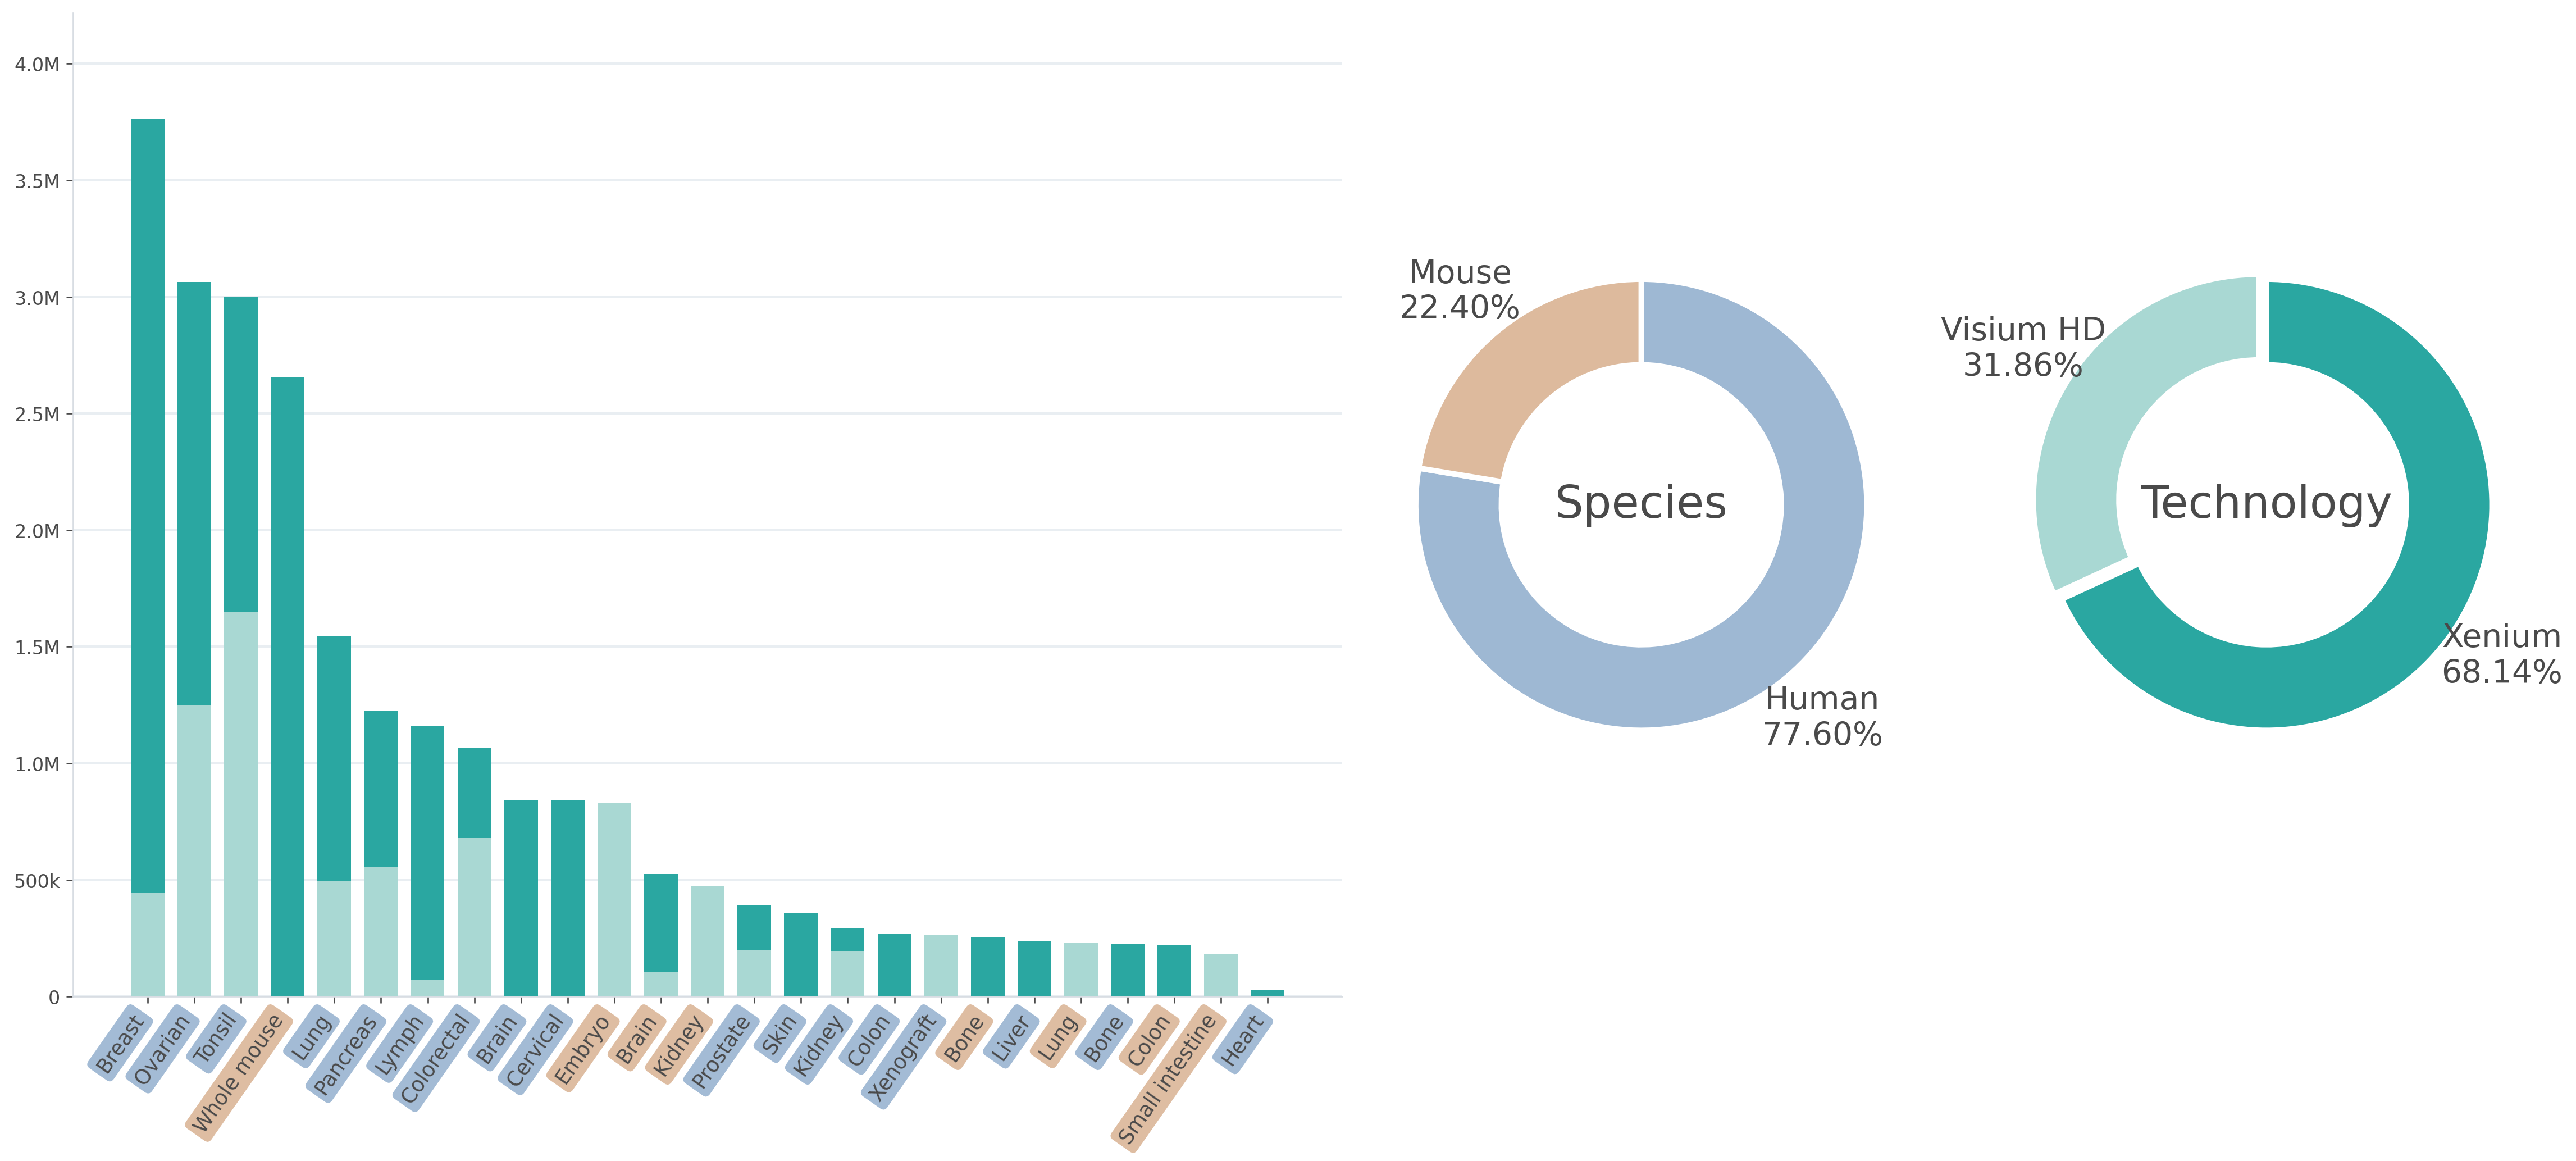
\includegraphics[width=0.98\linewidth]{dataset_dis.png}
\caption{Long-tail distribution of the frozen 22M release snapshot across 25
organ categories and 66 source studies. The expanded working manifest is
summarized separately in Table~\ref{tab:main_release_manifest}. The strong
imbalance across organs and platforms is one reason the benchmark is reported
regime-by-regime rather than as a single undifferentiated score.}
\label{fig:dataset_scale}
\end{figure*}

\begin{figure}[t]
\centering
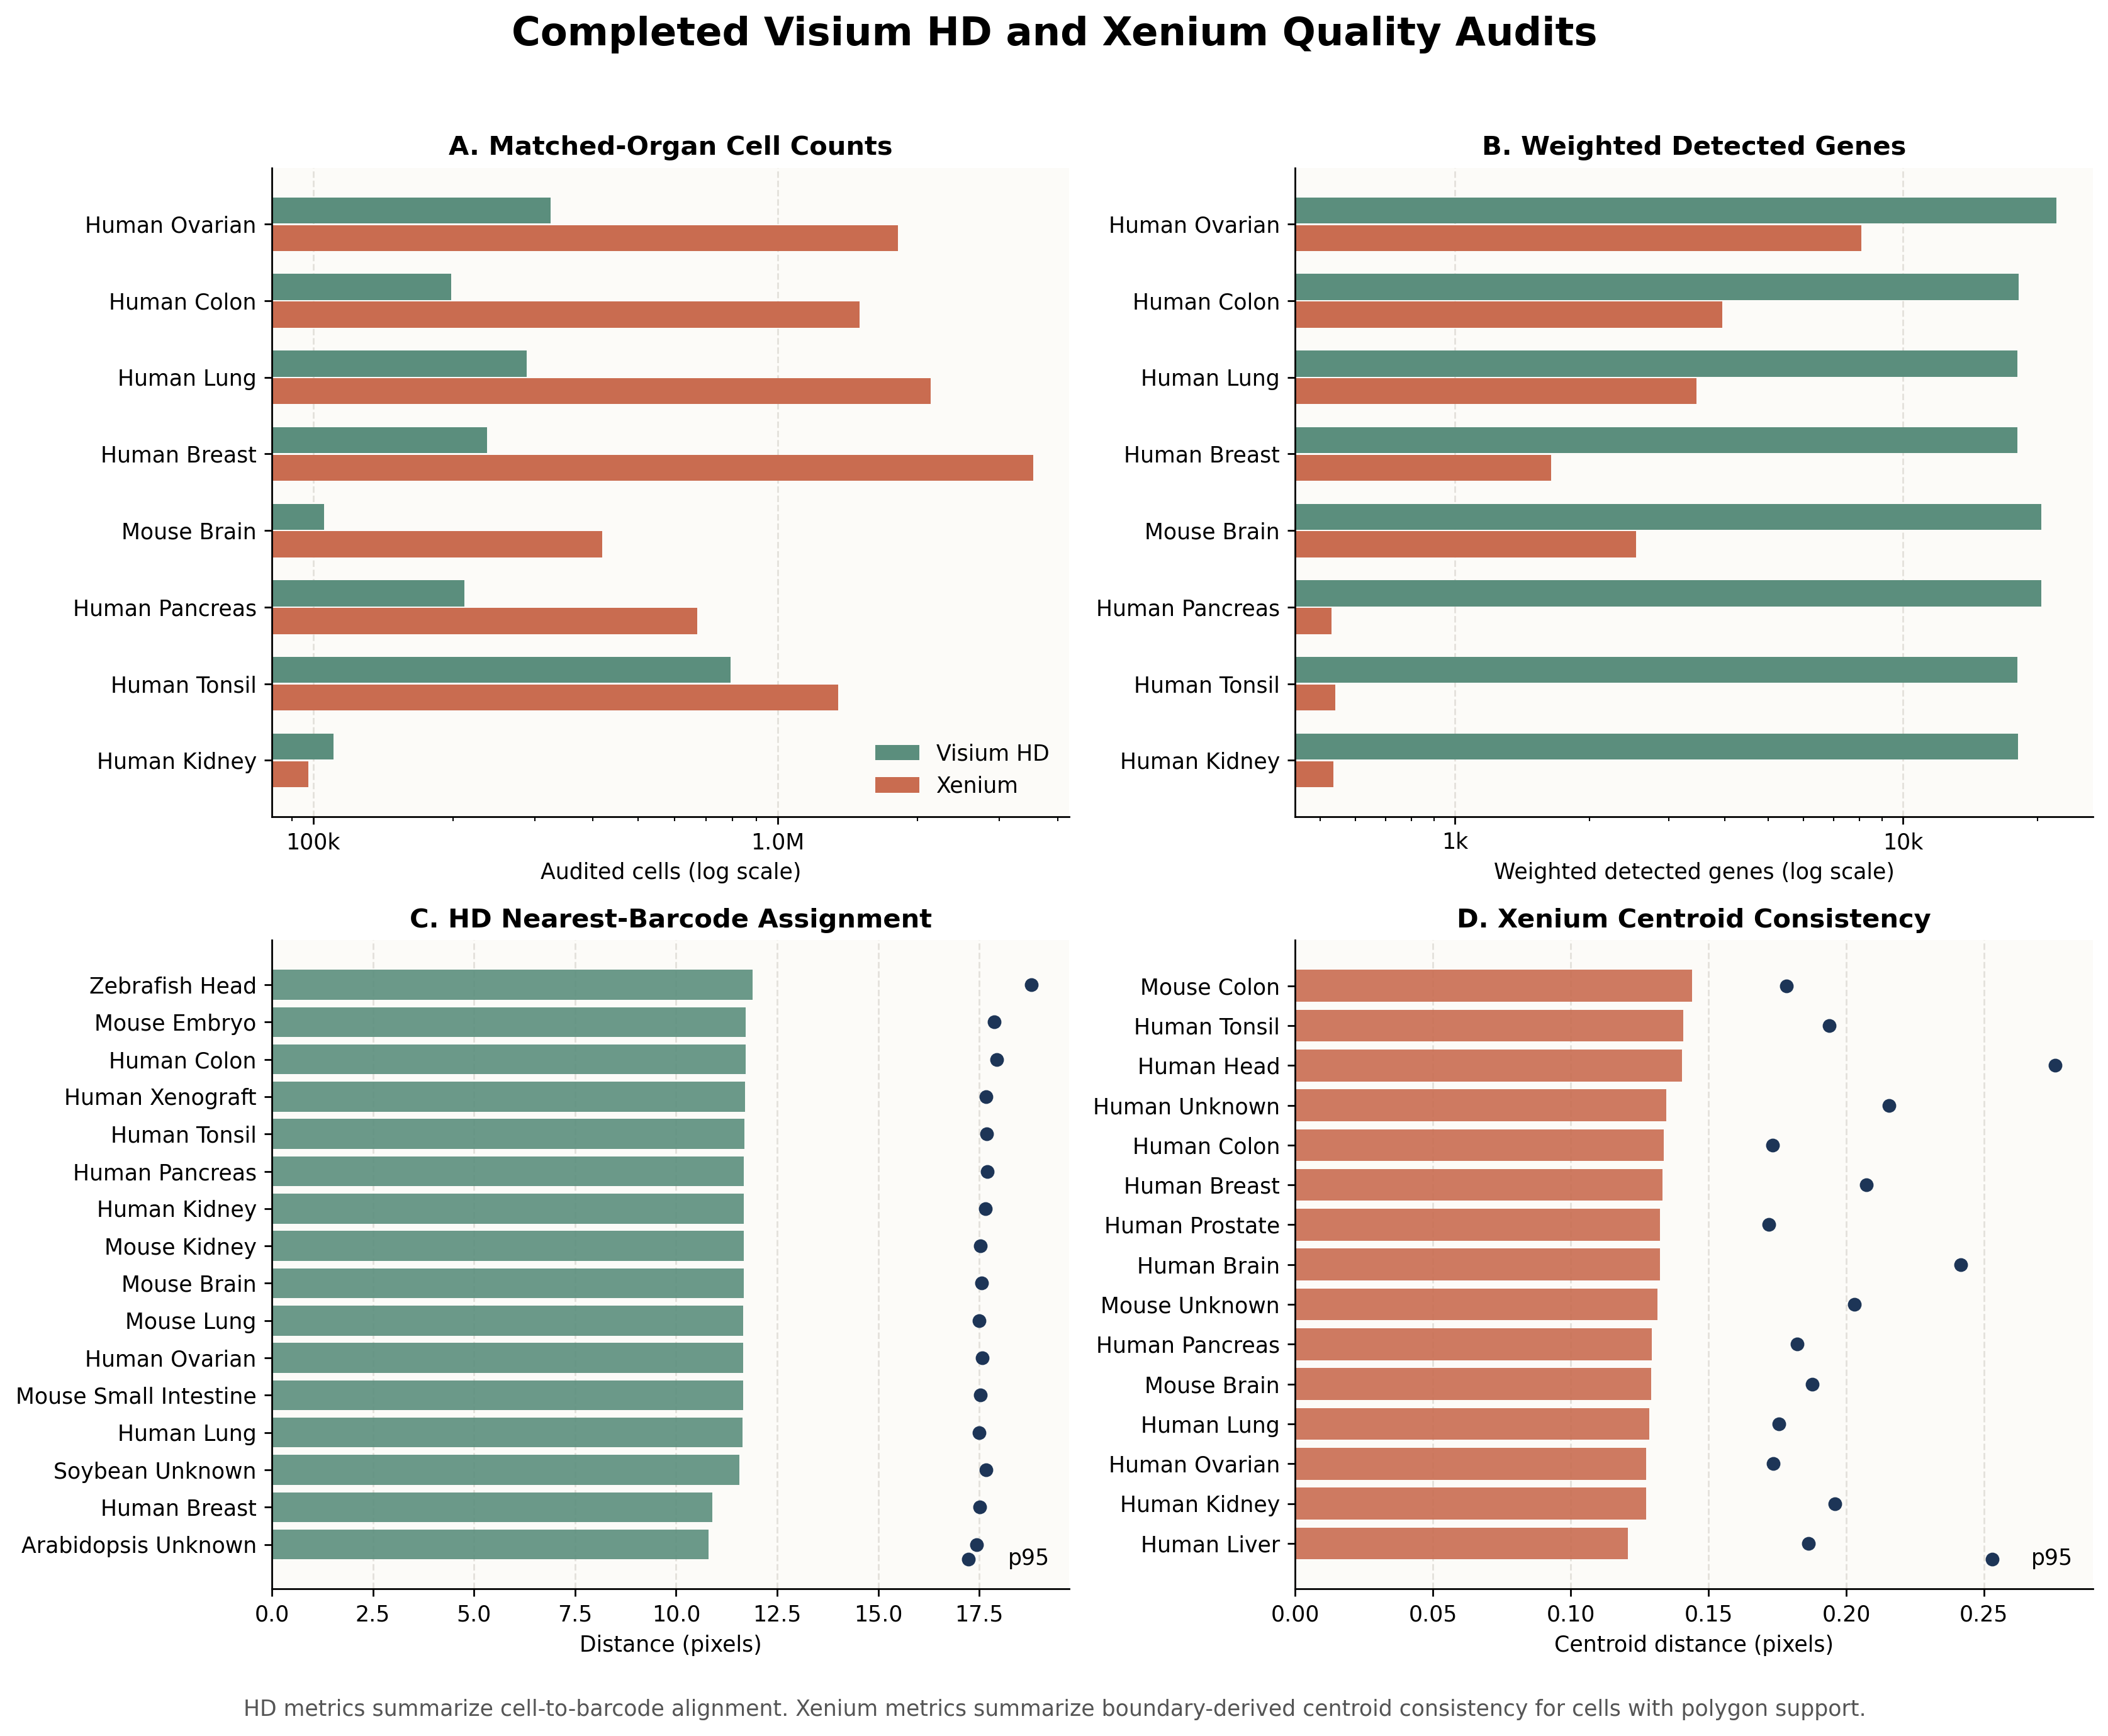
\includegraphics[width=0.98\linewidth]{platform_qc_overview.png}
\caption{Completed source-data quality audits used to vet the benchmark inputs. Top left: audited cell counts for the eight organs represented in both Visium HD and Xenium. Top right: weighted detected-gene counts for the same shared organs, showing the expected full-transcriptome HD panel versus variable Xenium panels. Bottom left: HD nearest-barcode assignment distances by organ, with median bars and p95 markers. Bottom right: Xenium centroid consistency by organ, with median bars and p95 markers computed from boundary-derived polygons whenever boundary support is available.}
\label{fig:platform_qc_overview}
\end{figure}

\subsection{Xenium Data Source}
\label{sec:comp_path}
\noindent
The \textbf{Xenium} dataset consists of high-resolution spatial transcriptomic data from multiple human and mouse tissues,
covering organs such as lung, pancreas, skin, liver, kidney, brain, and breast.
The data is generated using the Xenium in situ platform, capturing gene expression at subcellular resolution.
Overall, the Xenium dataset includes 28 collections, covering 12 million cells across 67,316 tissue patches.

For the benchmark, Xenium contributes the broader study diversity and the cross-platform evaluation targets. We currently curate 28 Xenium collections spanning human and mouse tissues, with panel sizes ranging from targeted 541-gene panels to larger 5K/custom panels with more than 10k genes. Platform-provided cell coordinates and segmentation masks are used whenever available to anchor cell-level crops in the histology frame. Because the Xenium panels are not uniform, cross-platform evaluation is defined on the \emph{intersection} of harmonized gene symbols between the train and test domains rather than on the union of all genes. For readability, we call the two native-Xenium human-lung-cancer targets \textbf{X1} and \textbf{X2}; internal source identifiers remain only in the machine-readable manifest. This shared-gene protocol yields 370 genes for X1 and 465 genes for X2 in the benchmarks reported later in the appendix.

\subsection{Visium HD Data Source}
\label{sec:st}
\noindent
The \textbf{Visium HD} dataset provides spatially resolved transcriptomic data from multiple tissue types,
including kidney, embryo, breast cancer, lung cancer, pancreas, and brain.
Unlike Xenium, Visium HD offers a higher-throughput approach for large-scale tissue analysis.
\\

\noindent
Together, the Xenium and Visium HD datasets form a comprehensive foundation for cell-level benchmarking, enabling systematic evaluation of foundation models for spatial transcriptomics across organs, species, and imaging resolutions.

For Visium HD we start from the native 2\,$\mu$m bin grid and the full-resolution histology image supplied by the platform. Bins are registered into the slide coordinate system using the official spatial transforms, after which a cell-segmentation stage defines candidate nuclei/cells in the same coordinate frame. Cell-level expression is then obtained by aggregating bin counts to segmented cells following the official 10x/bin2cell-style workflow: bins overlapping a segmented cell are assigned to that cell; boundary cases are resolved within the segmentation workflow before aggregation; and cells without stable spatial support or valid image context are removed before patch extraction. The resulting cell table is the unit used throughout the benchmark.

Platform harmonization is handled explicitly at evaluation time. Within-platform Visium HD experiments use the full 18,085-gene panel. Cross-platform evaluation is restricted to genes shared after gene-symbol harmonization between the train and test datasets, and the cached Xenium$\leftrightarrow$Visium runs additionally use shared-gene normalization before retrieval. In the completed appendix experiments this yields 465 shared genes for A$\!\rightarrow\!$X2 and 370 shared genes for A$\!\rightarrow\!$X1 and X1$\!\rightarrow\!$B.

\begin{figure*}[t]
\centering
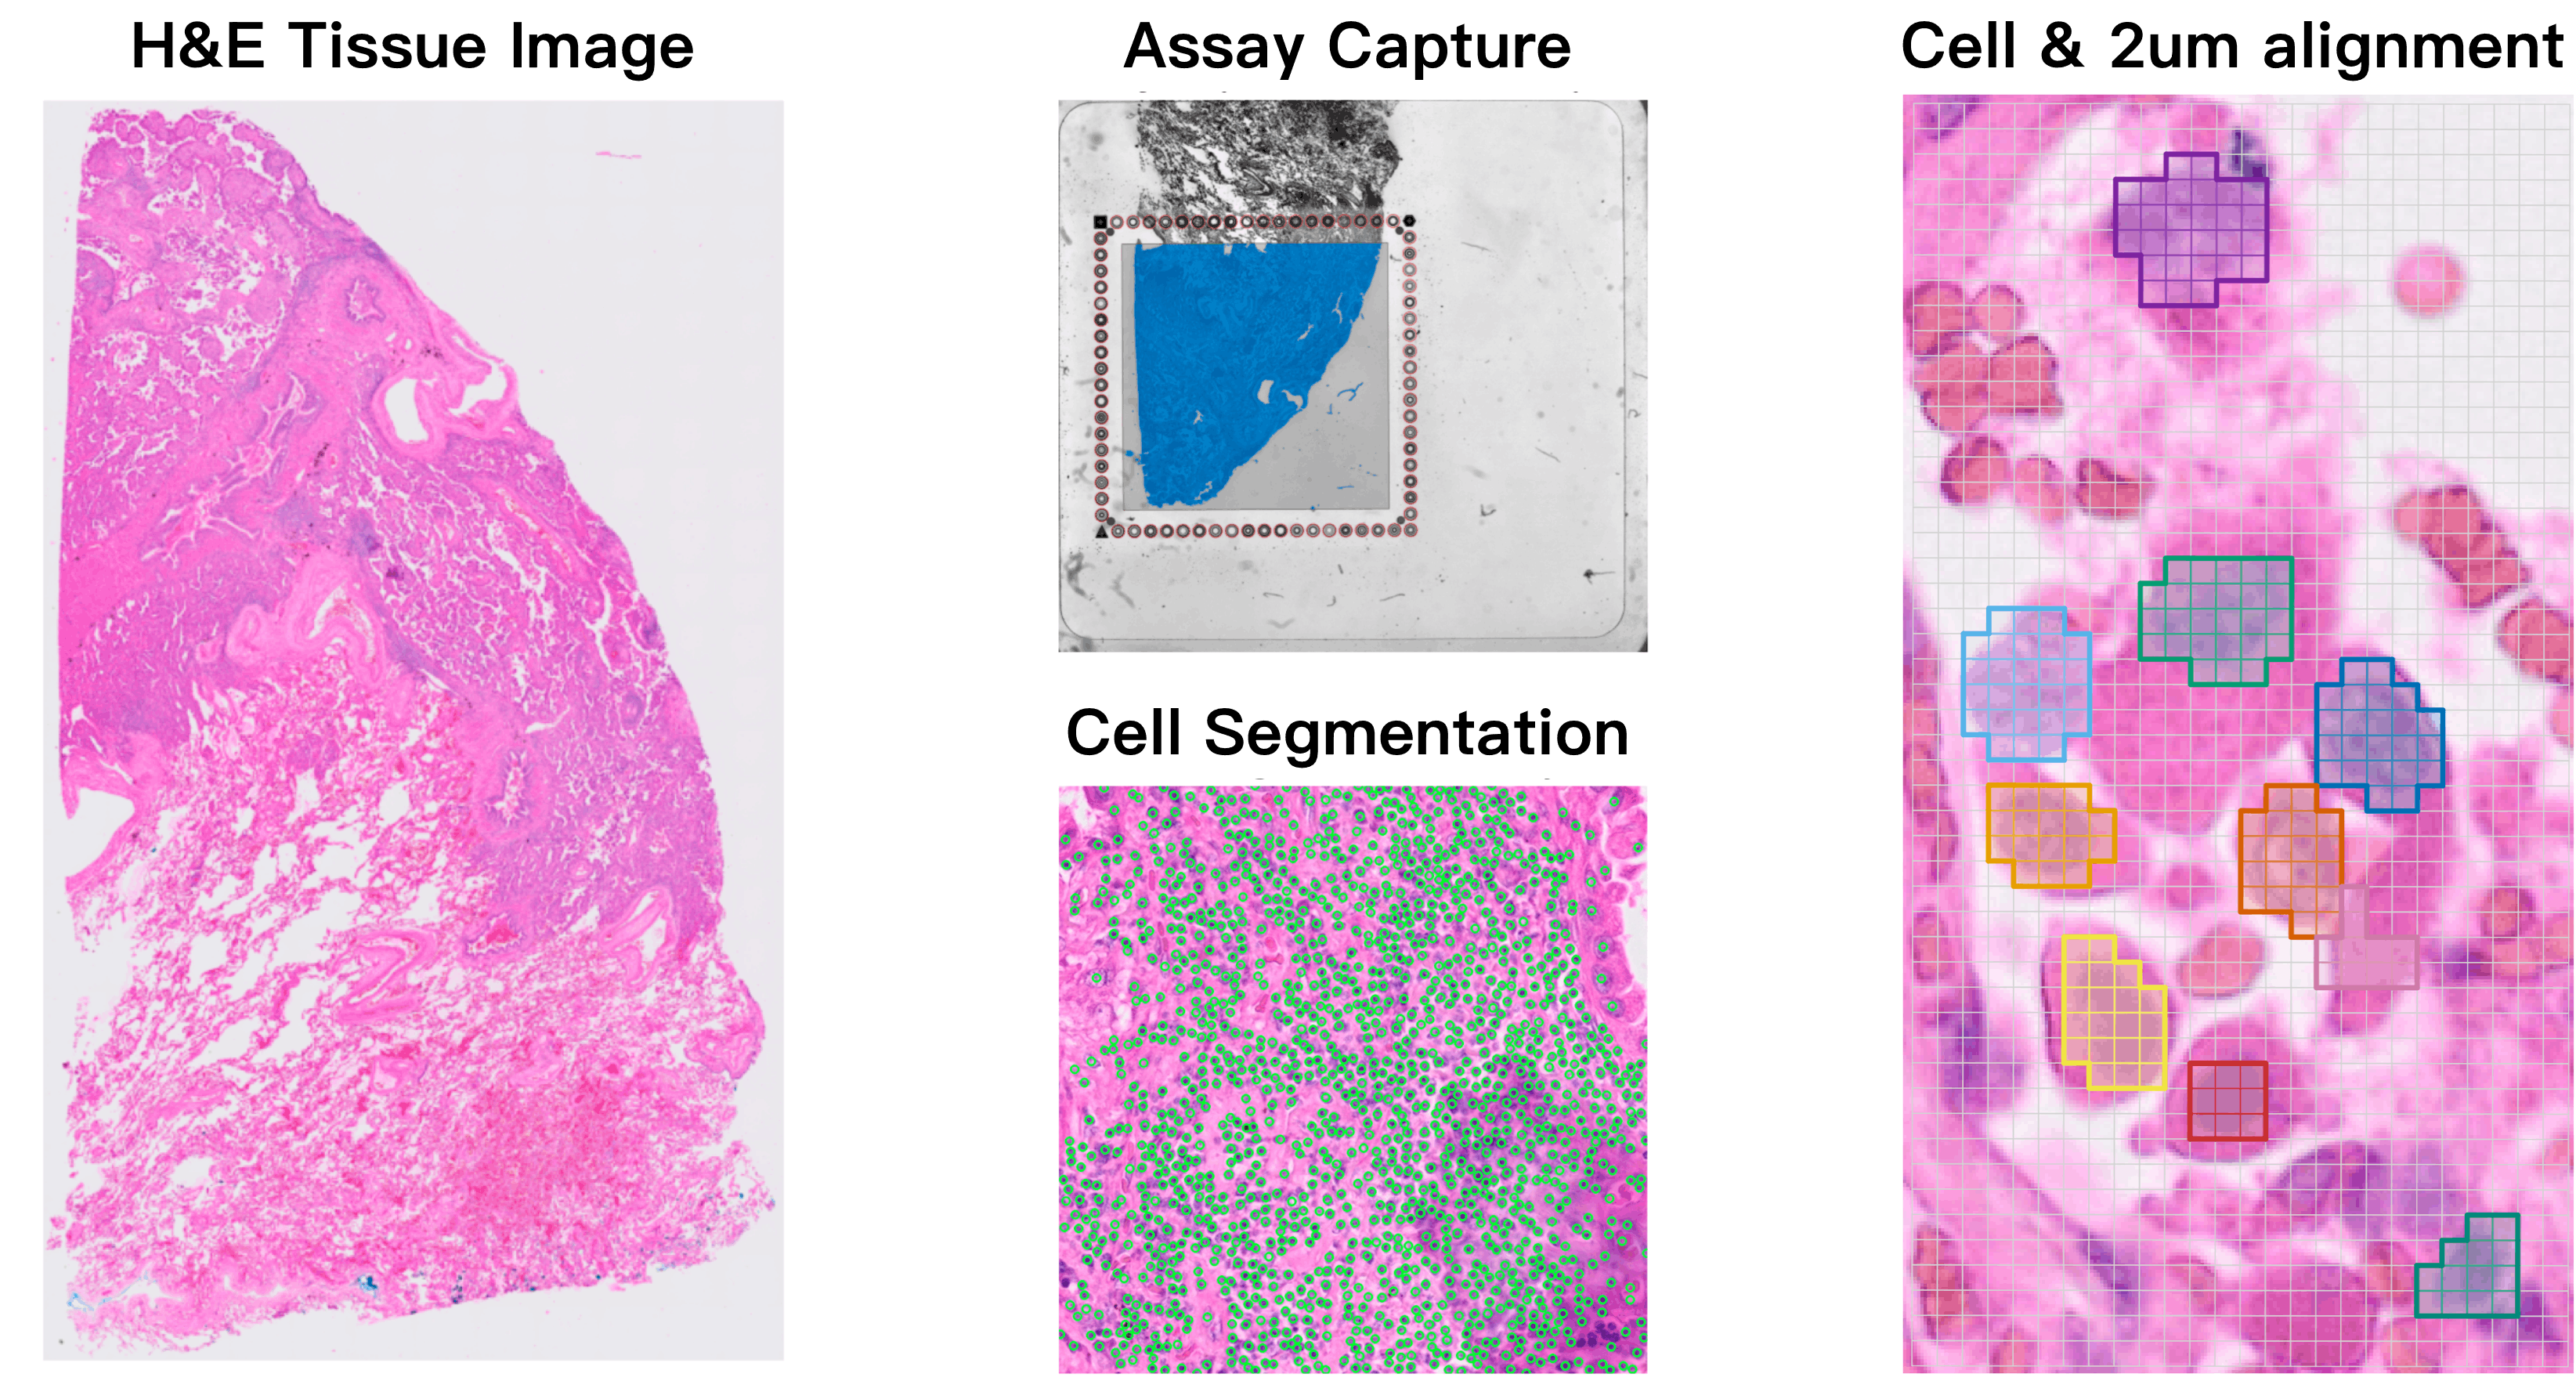
\includegraphics[width=0.98\linewidth]{cell_seg.png}
\caption{Visium HD bin-to-cell construction used by the benchmark. Starting from the native 2\,$\mu$m bins, we register molecular coordinates to the histology frame, segment cells/nuclei, aggregate overlapping bins to cells, and retain only cells that have both valid expression support and aligned image patches.}
\label{fig:bin2cell}
\end{figure*}

\subsection{In-house DBiC-seq data}
\label{sec:inhouse_dbic}
\noindent
The expanded manifest adds 21 in-house DBiC-seq samples spanning
mouse-embryo-, cervical-cancer-, and lung-cancer-derived cell-line settings.
DBiC-seq jointly measures spatial expression and paired cellular imaging on a
regular grid, so these records provide native cell targets rather than
Visium-HD-derived targets. Across the 21 samples, 54,304 cells were measured;
QC removed 315 cells lacking complete paired information, leaving 53,989
released aligned cells. These data account for 0.1907\% of the current
28,315,247-target manifest. They are therefore a small but genuinely new
primary-data contribution, complementary to the much larger aggregation of
public data. A broader in-house collection of approximately 200,000 paired
cells is under preparation but is not included in any count or result in this
paper.

\subsection{Benchmark support and complete public-source manifest}
\label{sec:benchmark_manifest}
The compact support table below defines the lung examples used in the
protocol-focused analyses, while
\Cref{tab:all_xenium_visium_summary} provides the complete public Xenium and
Visium HD source listing. Internal acquisition identifiers are intentionally
kept in the machine-readable manifest rather than used as biological labels in
the manuscript.

\begin{table*}[t]
\centering
\scriptsize
\setlength{\tabcolsep}{5pt}
\caption{Benchmark-support summary for the lung subsets instantiated in this appendix. ``Cross-patient'' denotes transfer between distinct samples under matched preprocessing; ``cross-platform'' denotes transfer between Visium HD and Xenium under shared-gene evaluation.}
\label{tab:benchmark_support}
\resizebox{\linewidth}{!}{%
\begin{tabular}{l l l c c c c}
\toprule
\textbf{Sample / study} & \textbf{Organ} & \textbf{Platform} & \textbf{Genes} & \textbf{In-domain} & \textbf{Cross-patient} & \textbf{Cross-platform} \\
\midrule
A & Human lung cancer & Visium HD & 18,085 & yes ($A\!\rightarrow\!A$) & yes ($A\!\rightarrow\!B$) & yes ($A\!\rightarrow\!$X1 / X2) \\
B & Human lung cancer & Visium HD & 18,085 & data available & yes (held-out target) & yes ($\leftarrow$X1) \\
X1: native-Xenium lung target 1 & Human lung cancer & Xenium & 541 & yes (X1$\!\rightarrow\!$X1) & n/a & yes (X1$\!\rightarrow\!B$) \\
X2: native-Xenium lung target 2 & Human lung cancer & Xenium & 541 & not used here & n/a & yes ($A\!\rightarrow\!$X2) \\
\bottomrule
\end{tabular}
}
\end{table*}

% ============ Data Table =============
\begin{table*}[t]
\centering
\scriptsize
\setlength{\tabcolsep}{2.8pt}
\renewcommand{\arraystretch}{0.94}
\caption{Comprehensive summary for Xenium and Visium HD datasets.
Collection names are simplified and grouped by species and platform. The tissue-patch column is omitted; \texttt{Num.genes} reports Xenium panel size or the processed whole-transcriptome Visium HD target size used in this benchmark.}
\label{tab:all_xenium_visium_summary}
\begin{tabularx}{\textwidth}{
>{\raggedright\arraybackslash}p{1.45cm}
>{\raggedright\arraybackslash}p{1.45cm}
>{\raggedright\arraybackslash}X
>{\raggedright\arraybackslash}p{1.75cm}
>{\raggedleft\arraybackslash}p{1.35cm}
>{\raggedleft\arraybackslash}p{1.35cm}}
\toprule
\textbf{Species} & \textbf{Platform} & \textbf{Sample Name} & \textbf{Organ Type} &
\makecell[r]{\textbf{Num.}\\\textbf{cell}} &
\makecell[r]{\textbf{Num.}\\\textbf{genes}} \\
\midrule
\multicolumn{6}{c}{\textbf{Human — Xenium}} \\
\midrule
Human & Xenium & Lung cancer (Tech Note; v1 + Prime 5K) & Lung & 278659 & 541 \\
Human & Xenium & Pancreatic cancer (Multi-Tissue panel) & Pancreatic & 190965 & 538 \\
Human & Xenium & Pancreas (Multimodal segmentation; FFPE) & Pancreas & 140702 & 541 \\
Human & Xenium & Tonsil (Multi-Tissue panel) & Tonsil & 1349620 & 541 \\
Human & Xenium & Skin (Multi-Tissue panel) & Skin & 68476 & 541 \\
Human & Xenium & Liver (Multi-Tissue panel) & Liver & 239271 & 541 \\
Human & Xenium & Heart (Multi-Tissue panel) & Heart & 26366 & 541 \\
Human & Xenium & Skin (Preview; custom add-on) & Skin & 87499 & 541 \\
Human & Xenium & Kidney (Preview; Multi-Tissue panel) & Kidney & 97560 & 541 \\
Human & Xenium & Lung cancer (Preview; Multimodal segmentation) & Lung & 162254 & 541 \\
Human & Xenium & Breast cancer (FFPE; 5K + 100 custom) & Breast & 699110 & 9475 \\
Human & Xenium & Ovarian adenocarcinoma (Fresh-frozen; 5K) & Ovarian glands & 1157659 & 10029 \\
Human & Xenium & Cervical cancer (FFPE; 5K + 100 custom) & Cervical & 840387 & 9475 \\
Human & Xenium & Skin melanoma (Preview; FFPE; 5K) & Skin & 112551 & 10017 \\
Human & Xenium & Prostate adenocarcinoma (Preview; FFPE; 5K) & Prostate & 193000 & 10017 \\
Human & Xenium & Lymph node (Preview; FFPE; 5K) & Lymph Node & 708983 & 11094 \\
Human & Xenium & Breast (FFPE; entire sample area) & Breast & 892966 & 541 \\
Human & Xenium & Breast (FFPE; custom add-on) & Breast & 574527 & 541 \\
Human & Xenium & Ovarian cancer (FFPE; Immuno-Oncology + custom) & Ovarian & 247636 & 541 \\
Human & Xenium & Lung cancer (FFPE; Immuno-Oncology + custom) & Lung & 161000 & 541 \\
Human & Xenium & Pancreatic ductal adenocarcinoma (FFPE; Immuno-Oncology) & Pancreatic duct gland & 235099 & 541 \\
Human & Xenium & Colorectal cancer (FFPE; Immuno-Oncology + custom) & Colorectal & 388175 & 541 \\
Human & Xenium & Brain cancer (FFPE; Immuno-Oncology + custom) & Brain & 816769 & 541 \\
\midrule
\multicolumn{6}{c}{\textbf{Mouse — Xenium}} \\
\midrule
Mouse & Xenium & Colon (Fresh-frozen; Multimodal segmentation) & Colon & 219797 & 541 \\
Mouse & Xenium & Whole pup (Preview; Atlassing panel) & Multi & 1355849 & 541 \\
Mouse & Xenium & Whole pup (FFPE; 5K + Snap25a/b add-on) & Multi & 298870 & 13780 \\
Mouse & Xenium & Brain hemisphere (Fresh-frozen; 5K) & Brain & 63173 & 13780 \\
Mouse & Xenium & Bone (Custom add-on panel) & Bone & 253560 & 541 \\
\midrule
\multicolumn{6}{c}{\textbf{Human — Visium HD}} \\
\midrule
Human & Visium HD & Lung cancer (Fixed-frozen) & Lung & 325262 & 18{,}085 \\
Human & Visium HD & Pancreas (FFPE) & Pancreas & 88120 & 18{,}085 \\
Human & Visium HD & Tonsil (Fresh-frozen) & Tonsil & 1625450 & 18{,}085 \\
Human & Visium HD & Breast cancer (Fixed-frozen) & Breast & 433554 & 18{,}085 \\
Human & Visium HD & Lung cancer (Post-Xenium; FFPE) & Lung & 172049 & 18{,}085 \\
Human & Visium HD & Breast cancer (Fresh-frozen; Ultima sequencing) & Breast & 8492 & 18{,}085 \\
Human & Visium HD & Breast cancer (IF; FFPE) & Breast & 5000 & 18{,}085 \\
Human & Visium HD & Kidney (FFPE) & Kidney & 195320 & 18{,}085 \\
Human & Visium HD & Lymph node (FFPE) & Lymph Node & 73257 & 18{,}085 \\
Human & Visium HD & Prostate cancer (FFPE) & Prostate & 199766 & 18{,}085 \\
Human & Visium HD & Tonsil (Fresh-frozen; Ultima sequencing) & Tonsil & 24349 & 18{,}085 \\
Human & Visium HD & Colorectal cancer (FFPE) & Colorectal & 679635 & 18{,}085 \\
Human & Visium HD & Ovarian cancer (Fresh-frozen; cross-platform) & Ovarian & 86782 & 18{,}085 \\
Human & Visium HD & Pancreatic cancer (Fresh-frozen; 3') & Pancreas & 467536 & 18{,}085 \\
Human & Visium HD & Ovarian cancer (Fresh-frozen; cross-platform; 3') & Ovarian & 145780 & 18{,}085 \\
Human & Visium HD & Ovarian cancer (Fresh-frozen; 3') & Ovarian & 1017702 & 18{,}085 \\
\midrule
\multicolumn{6}{c}{\textbf{Mouse — Visium HD}} \\
\midrule
Mouse & Visium HD & Kidney (FFPE) & Kidney & 253032 & 18{,}085 \\
Mouse & Visium HD & Embryo (FFPE) & Embryo & 84507 & 18{,}085 \\
Mouse & Visium HD & Brain (Fixed-frozen) & Brain & 52491 & 18{,}085 \\
Mouse & Visium HD & Lung (Fresh-frozen) & Lung & 229111 & 18{,}085 \\
Mouse & Visium HD & Small intestine (FFPE) & Small Intestine & 181224 & 18{,}085 \\
Mouse & Visium HD & Brain (Fresh-frozen; 3') & Brain & 54434 & 18{,}085 \\
Mouse & Visium HD & Embryo (Fresh-frozen; 3') & Embryo & 743876 & 18{,}085 \\
Mouse & Visium HD & Kidney (Fresh-frozen; 3') & Kidney & 219225 & 18{,}085 \\
\midrule
\multicolumn{6}{c}{\textbf{Human + Mouse Xenograft — Visium HD}} \\
\midrule
Human + Mouse Xenograft & Visium HD & Human + mouse xenograft (Fresh-frozen; 3') & Xenograft & 263743 & 18{,}085 \\
\midrule
\multicolumn{6}{c}{\textbf{Arabidopsis thaliana — Visium HD}} \\
\midrule
Arabidopsis thaliana & Visium HD & Arabidopsis thaliana (Fresh-frozen; 3') & Plant & 58 & 18{,}085 \\
\midrule
\multicolumn{6}{c}{\textbf{Rhesus macaque — Visium HD}} \\
\midrule
Rhesus macaque & Visium HD & Kidney (Fresh-frozen; 3') & Kidney & 101262 & 18{,}085 \\
\midrule
\multicolumn{6}{c}{\textbf{Soybean — Visium HD}} \\
\midrule
Soybean & Visium HD & Seed (Fresh-frozen; 3') & Seed & 8566 & 18{,}085 \\
\midrule
\multicolumn{6}{c}{\textbf{Zebrafish — Visium HD}} \\
\midrule
Zebrafish & Visium HD & Head (Fresh-frozen; 3') & Head & 54251 & 18{,}085 \\
\bottomrule
\end{tabularx}
\end{table*}

\subsection{Completed quality audits for Visium HD and Xenium}
\label{sec:source_quality_audits}
Before treating the release as a benchmark rather than a loose data collection, we audited both source platforms for the specific failure modes that would most directly invalidate downstream evaluation. For Visium HD, the critical checks are whether aligned cells remain stably anchored to in-tissue barcodes and whether large context crops frequently fall off the tissue boundary. For Xenium, the critical checks are whether cell centroids remain consistent with polygon-derived boundaries when those boundaries are available, whether crop extraction stays within the morphology frame, and whether matching-organ gene overlap with HD is large enough to support fair shared-gene evaluation.

Table~\ref{tab:platform_qc_summary} summarizes the completed audits. The HD audit covers 24 complete samples across 16 organ groups and 10M aligned cells. Organ-level median assignment distance stays in a narrow 10.81--11.89 pixel range, and the mean 224-pixel crop edge rate is effectively zero ($2.95\times10^{-6}$). The Xenium audit covers 42 complete samples across 15 organ groups and 12M detected cells. For samples with polygon support, median centroid inconsistency stays between 0.12 and 0.14 pixels, while the mean 224-pixel crop edge rate remains low at 0.00541. For HD, the weighted top-200 gene fraction ranges from 0.154 to 0.691 across organs, which indicates organ-dependent concentration differences but not an obvious collapse of molecular support.

\begin{table*}[t]
\centering
\scriptsize
\setlength{\tabcolsep}{3.2pt}
\caption{Platform-level summary of the completed source-data quality audits. HD metrics come from cell-to-nearest-barcode alignment; Xenium centroid metrics are computed only for samples with polygon boundary support.}
\label{tab:platform_qc_summary}
\begin{tabularx}{\textwidth}{
l c c r
>{\raggedright\arraybackslash}p{2.6cm}
>{\raggedright\arraybackslash}p{3.2cm}
>{\raggedright\arraybackslash}X}
\toprule
\textbf{Platform} & \textbf{Samples} & \textbf{Organs} & \textbf{Cells} & \textbf{Weighted genes} & \textbf{Spatial consistency} & \textbf{Cross-platform overlap} \\
\midrule
Visium HD & 24 & 16 & 3.72M & 18.0k--41.0k & assignment dist. 10.81--11.89 px & reference full-gene panel for the 8 organs shared with Xenium \\
Xenium & 42 & 15 & 16.31M & 484--8,090 & centroid dist. 0.12--0.14 px & 368--4,340 shared genes vs matching-organ HD \\
\bottomrule
\end{tabularx}
\end{table*}

%-------from table 3 to Table S5--------
\begin{table*}[!t]
\centering
\scriptsize
\setlength{\tabcolsep}{2.4pt}
\renewcommand{\arraystretch}{0.98}
\setlength{\abovecaptionskip}{4pt}
\setlength{\belowcaptionskip}{3pt}

\caption{\textbf{Reviewer-accessible artifacts and reproducibility checklist.}
Artifacts supporting download, inspection, and reproduction during review. File sizes, checksums, and release tags are recorded in the released checksum manifest.}
\label{tab:S5_review_artifact_checklist}

\begin{tabularx}{\textwidth}{
>{\raggedright\arraybackslash}p{1.75cm}
>{\raggedright\arraybackslash}p{2.15cm}
>{\raggedright\arraybackslash}X
>{\raggedright\arraybackslash}p{2.05cm}
>{\raggedright\arraybackslash}X
}
\toprule
\textbf{Artifact} &
\textbf{Access} &
\textbf{Contents} &
\textbf{Integrity / version} &
\textbf{Reproduction command or use} \\
\midrule

Full manifest &
\makecell[l]{\texttt{manifest/}\\
\texttt{full\_release\_}\\
\texttt{manifest.csv}} &
Source IDs, platform, species, organ, sample name, cell count, gene target, inclusion flag, source, license, and QC status &
\makecell[l]{Release tag\\
\texttt{MANIFEST}\\
\texttt{.sha256}} &
Audit scale, platform composition, organ coverage, and inclusion/exclusion decisions \\

Review subset &
\makecell[l]{\texttt{review\_}\\
\texttt{subset/}} &
Lightweight crops, expression files, metadata, and split files using the full-release schema &
\makecell[l]{Subset manifest\\
\texttt{MANIFEST}\\
\texttt{.sha256}} &
\makecell[l]{\texttt{bash scripts/}\\
\texttt{run\_smoke\_test.sh}\\
\texttt{--config configs/}\\
\texttt{review\_subset.yaml}} \\

Benchmark splits &
\texttt{splits/} &
Fixed CSV/JSON splits for $A\!\to\!A$, $A\!\to\!B$, age-shift, and cross-platform protocols &
\makecell[l]{Commit hash\\
Checksum\\
manifest} &
\makecell[l]{\texttt{python scripts/}\\
\texttt{check\_splits.py}\\
\texttt{--manifest manifest/}\\
\texttt{full\_release\_}\\
\texttt{manifest.csv}} \\

Evaluation code &
\makecell[l]{\texttt{scripts/}\\
\texttt{configs/}} &
Loaders, metrics, retrieval baselines, STBoost configs, and plotting utilities &
\makecell[l]{Commit hash\\
Package\\
versions} &
\makecell[l]{\texttt{python scripts/}\\
\texttt{eval\_gene\_}\\
\texttt{prediction.py}\\
\texttt{--config configs/}\\
\texttt{bench\_aa.yaml}} \\

Environment &
\makecell[l]{\texttt{environment.}\\
\texttt{yml}\\
\texttt{Dockerfile}} &
Python, package, model-loading, and plotting dependencies &
\makecell[l]{Environment lock\\
Release tag} &
\makecell[l]{\texttt{conda env create}\\
\texttt{-f environment.}\\
\texttt{yml}} \\

Croissant metadata &
\makecell[l]{\texttt{metadata/}\\
\texttt{croissant.json}} &
Machine-readable dataset description, responsible-use notes, license fields, and download pointers &
\makecell[l]{Validator log\\
Release tag} &
Dataset-card validation and metadata inspection \\

Figure/table scripts &
\makecell[l]{\texttt{scripts/}\\
\texttt{figures/}} &
Scripts for regenerating benchmark tables and representative panels from release or review-subset outputs &
\makecell[l]{Commit hash\\
Expected-output\\
log} &
\makecell[l]{\texttt{python scripts/}\\
\texttt{figures/}\\
\texttt{make\_main\_}\\
\texttt{tables.py}\\
\texttt{--config configs/}\\
\texttt{review\_subset.yaml}} \\

\bottomrule
\end{tabularx}
\end{table*}
%------------------------------------

The matched-organ comparison in Figure~\ref{fig:platform_qc_overview} and Table~\ref{tab:platform_qc_shared_organs} supports the first cross-platform benchmark package already reported in this appendix. Human ovarian, colon, lung, and breast tissues all retain more than one thousand harmonized genes on average between Xenium and matching-organ HD, while pancreas, tonsil, and kidney still support smaller but nontrivial shared-gene evaluations. This organ dependence is exactly why the benchmark is reported regime-by-regime rather than as a single pooled cross-platform score.

\begin{table*}[t]
\centering
\scriptsize
\setlength{\tabcolsep}{5pt}
\caption{Matched-organ HD/Xenium audit comparison for the eight organs represented in both completed audits. ``HD genes'' and ``Xenium genes'' denote weighted detected-gene counts from the corresponding organ-level audits; ``shared genes'' denotes the mean number of harmonized genes between Xenium samples and matching-organ HD collections.}
\label{tab:platform_qc_shared_organs}
\resizebox{\linewidth}{!}{%
\begin{tabular}{l c c r r r r r}
\toprule
\textbf{Organ} & \textbf{HD samples} & \textbf{Xenium samples} & \textbf{HD cells} & \textbf{Xenium cells} & \textbf{HD genes} & \textbf{Xenium genes} & \textbf{Shared genes} \\
\midrule
Human Ovarian & 3 & 3 & 323,975 & 1,812,419 & 22,028 & 8,090 & 4,340 \\
Human Colon & 1 & 3 & 198,193 & 1,499,546 & 18,118 & 3,949 & 2,930 \\
Human Lung & 2 & 7 & 288,383 & 2,135,129 & 18,031 & 3,457 & 1,726 \\
Human Breast & 2 & 6 & 237,065 & 3,544,324 & 18,024 & 1,641 & 1,236 \\
Mouse Brain & 2 & 4 & 105,733 & 418,344 & 20,346 & 2,537 & 968 \\
Human Pancreas & 2 & 4 & 211,731 & 670,667 & 20,366 & 531 & 400 \\
Human Tonsil & 1 & 1 & 790,670 & 1,349,620 & 18,009 & 541 & 370 \\
Human Kidney & 1 & 1 & 110,711 & 97,560 & 18,043 & 535 & 368 \\
\bottomrule
\end{tabular}
}
\end{table*}

\subsection{Dataset construction and alignment pipeline}
\label{sec:construction_alignment}
The benchmark-ready pipeline follows the same high-level stages across studies: (1) source download and metadata audit; (2) slide- and section-level eligibility checks; (3) coordinate registration between histology and molecular coordinates; (4) cell segmentation or use of platform-provided masks; (5) multi-scale patch extraction centered on each retained cell; (6) expression assignment and gene-symbol harmonization; (7) benchmark split generation; and (8) optional generation of captions and communication-graph summaries. The key design choice is that the final released unit is always a \emph{cell} with aligned morphology, coordinates, and expression, even when the upstream technology is spot/bin based.

\FloatBarrier

\subsection{Data schema and release package}
\label{sec:release_schema}
The benchmark release is organized around a small number of reusable artifact types. Multi-scale image crops and aligned expression matrices are paired through cell identifiers; metadata tables provide organ/platform/sample/study fields and spatial coordinates; split files define train/validation/test membership; and evaluation scripts consume the same processed release used to produce the appendix results. The review package focuses on the assets needed to inspect the protocol, while the full release keeps the same schema and versioning conventions.

\begin{table}[H]
\centering
\scriptsize
\setlength{\tabcolsep}{5pt}
\caption{Main artifact types in the \dataset benchmark release.}
\label{tab:data_schema}
\begin{tabularx}{\linewidth}{
>{\raggedright\arraybackslash}p{2.65cm}
>{\raggedright\arraybackslash}X}
\toprule
\textbf{Artifact} & \textbf{Format, unit, status, and contents} \\
\midrule
Histology patches & PNG/TIFF; cell; required. Cell crop plus larger local-context crops. \\
Expression matrices & H5AD/CSV/NumPy; cell \(\times\) gene; required. Processed targets used for training and evaluation. \\
Metadata tables & CSV/JSON; cell or sample; required. Organ, platform, study, sample, coordinates, and split membership. \\
Split definitions & CSV/JSON; cell or sample; required. In-domain, cross-patient, and cross-platform partitions. \\
Configs and scripts & Python/YAML/shell; experiment; required. Loaders, evaluation, plotting, and job scripts. \\
Auxiliary annotations & CSV/JSON; cell or neighborhood; optional. Captions, communication summaries, and downstream labels. \\
\bottomrule
\end{tabularx}
\end{table}

\section{Supplementary Benchmark and Analysis Results}
\label{sec:supplementary_results}
\subsection{Reviewer-motivated validation and stress tests}
\label{sec:reviewer_validation}

\noindent\textbf{Common protocol.}
The new native-Xenium campaign uses 30 samples, at most 12{,}000 spatially
sampled cells per sample, four contiguous edge holdouts, and a 5\%
coordinate-span train--test buffer. Target genes are selected from the training
partition only. Samples, rather than cells, are used for macro averaging,
bootstrap confidence intervals, and paired tests.

\noindent\textbf{Biological calibration.}
Training-selected marker/HVG overlap and cell-type-stratified pseudobulk
profiles calibrate whole-panel correlations at aggregate biological levels
(\Cref{tab:appendix_biological_calibration}).

\begin{table}[H]
\centering
\small
\setlength{\tabcolsep}{3.2pt}
\caption{\textbf{Biological calibration across 30 native-Xenium samples.}
Lower is better for pseudobulk RMSE; higher is better otherwise.}
\label{tab:appendix_biological_calibration}
\begin{tabular}{lrrrr}
\toprule
Readout & Image & Coord. & KNN & Mean \\
\midrule
Marker/HVG Gene Pearson & 0.201 & 0.031 & 0.028 & 0.000 \\
Cell-type pseudobulk RMSE & 0.120 & 0.224 & 0.187 & 0.188 \\
\bottomrule
\end{tabular}
\end{table}

\noindent\textbf{Ovarian age-associated shift case study.}
We compare transfer from an ovarian sample in the 60+ age band to either a
second 60+ sample or a younger-than-40 sample. Under the age-shifted setting,
F1 decreases from \(0.289\) to \(0.072\), gene-wise Spearman from \(0.036\) to
\(0.006\), and cell-wise Spearman from \(0.206\) to \(0.095\)
(\Cref{fig:ovarian_age_effect}). The predicted active-gene rate also falls from
\(0.166\) to \(0.027\). Because age is nested within sample and the molecular
panels differ, this is an age-associated, sample-confounded stress test rather
than a causal estimate of an age effect. The lower global distribution
distances in the age-shifted case further show that distribution proximity
alone does not guarantee preservation of predictive signal.

\begin{figure}[!t]
\centering
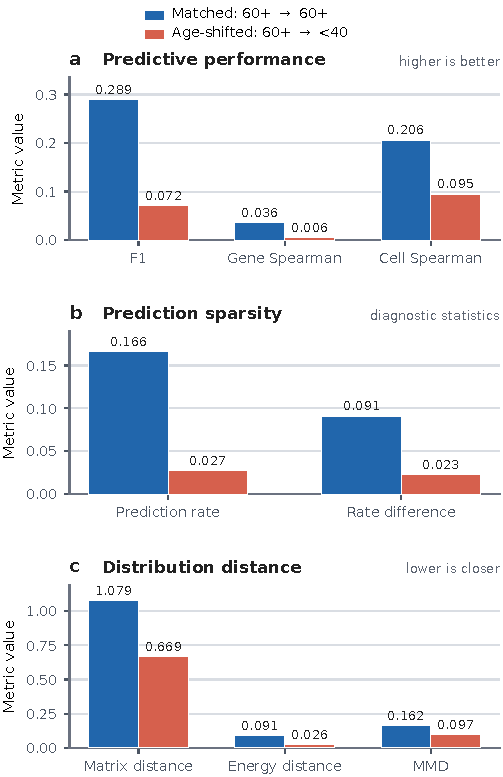
\includegraphics[width=\columnwidth]{ovarian_age_effect_single_column.pdf}
\caption{\textbf{Ovarian age-associated transfer case study.}
The same 60+ source sample is evaluated on a matched 60+ target (blue) and a
younger-than-40 target (orange). (a) Predictive performance falls under the
age-shifted transfer. (b) The active-gene prediction rate also collapses.
(c) Lower global distances do not track the loss of F1 and rank correlation.
The comparison is sample-confounded and is not evidence of a causal age
effect. Exact plotted values are provided with the figure-generation script.}
\label{fig:ovarian_age_effect}
\end{figure}

\noindent\textbf{Training-size sensitivity.}
On a non-diseased human-heart Xenium sample, all seven frozen encoders improve
monotonically as the training fraction increases
(\Cref{tab:appendix_encoder_training_size}). This reproduces the scale trend
under a stricter spatially buffered split without exposing the internal sample
identifier in the manuscript.

\begin{table}[H]
\centering
\small
\setlength{\tabcolsep}{4pt}
\caption{\textbf{Gene-macro Pearson versus training fraction on a
non-diseased human-heart Xenium sample.} Values average four spatial
holdouts.}
\label{tab:appendix_encoder_training_size}
\begin{tabular}{lrrrr}
\toprule
Encoder & 5\% & 10\% & 25\% & 100\% \\
\midrule
ResNet-50 & .140 & .160 & .190 & .221 \\
CTransPath & .162 & .186 & .222 & .259 \\
Phikon & .168 & .200 & .237 & .273 \\
CONCH & .178 & .213 & .256 & .292 \\
UNI & .188 & .218 & .259 & .295 \\
UNI2 & .197 & .225 & .257 & .295 \\
H-Optimus-0 & .205 & .233 & .269 & .307 \\
\bottomrule
\end{tabular}
\end{table}

\noindent\textbf{Same-organ sample-held-out transfer.}
Across 18 native-Xenium targets, the image model reaches Gene Pearson 0.170,
Cell Pearson 0.275, and F1 0.125, versus approximately zero, 0.205, and 0.031
for the training mean (\Cref{tab:appendix_sample_transfer}). Gene Pearson
ranges from 0.016 to 0.372. Because donor identifiers are incomplete, this
experiment is sample-held-out rather than patient-held-out.

\begin{table}[H]
\centering
\small
\caption{\textbf{Same-organ leave-one-sample-out macro across 18 targets.}}
\label{tab:appendix_sample_transfer}
\begin{tabular}{lrrrr}
\toprule
Model & Gene P. & Gene S. & Cell P. & F1 \\
\midrule
Image & .170 & .152 & .275 & .125 \\
Training mean & .000 & -- & .205 & .031 \\
\bottomrule
\end{tabular}
\end{table}

\noindent\textbf{Method-breadth negative result.}
We also implemented the official BLEEP projection, contrastive loss, and
top-50 retrieval design on the same frozen CONCH inputs. This algorithm adapter
underperforms the Ridge head in the spatially buffered benchmark
(\Cref{tab:appendix_bleep_negative}); it is therefore reported as a negative
method-breadth result rather than used in the main-text superiority claim.

\begin{table}[H]
\centering
\small
\caption{\textbf{BLEEP algorithm adapter versus Ridge across 30
native-Xenium samples.}}
\label{tab:appendix_bleep_negative}
\begin{tabular}{lrrr}
\toprule
Metric & BLEEP adapter & Ridge & Difference \\
\midrule
Gene Pearson & .293 & .324 & -.031 \\
F1 & .378 & .413 & -.035 \\
\bottomrule
\end{tabular}
\end{table}

\noindent\textbf{Pseudo-spot controls.}
\Cref{tab:appendix_pseudospot} gives the matched six-sample summary mentioned in
the main text. At full density, 55-\(\mu\)m regions in dense human lung contain
mixed predicted cell types in 55.5--66.4\% of regions and include
73.8--81.0\% of evaluated cells. The corresponding non-diseased human-heart
ranges are only 3.5--4.1\% and 7.0--8.3\%.

\begin{table}[H]
\centering
\small
\caption{\textbf{Matched cell-versus-pseudo-spot Gene Pearson across six
native-Xenium samples.}}
\label{tab:appendix_pseudospot}
\begin{tabular}{lrrrr}
\toprule
Evaluation unit & Cell & 8 \(\mu\)m & 16 \(\mu\)m & 55 \(\mu\)m \\
\midrule
Gene Pearson & .365 & .365 & .363 & .330 \\
\bottomrule
\end{tabular}
\end{table}

\noindent\textbf{Erosion/dilation sensitivity.}
The registration-shift results in \Cref{tab:main_hd_sensitivity} are the least
disruptive perturbation. Erosion and dilation change bin membership and UMI
totals more substantially (\Cref{tab:appendix_hd_boundary}). This result
motivates the explicit derived-target label and per-sample QC.

\begin{table}[H]
\centering
\small
\setlength{\tabcolsep}{3pt}
\caption{\textbf{Visium HD erosion/dilation sensitivity.} Values are
dilation/erosion medians over 3{,}000 polygons per example.}
\label{tab:appendix_hd_boundary}
\begin{tabular}{lrrr}
\toprule
Example & Bin Jaccard & Expr. cosine & \(|\Delta\mathrm{UMI}|\) \\
\midrule
Human lung & .622/.500 & .938/.877 & 61.0/51.0\% \\
Mouse brain & .720/.667 & .906/.871 & 37.3/32.8\% \\
Human pancreas & .600/.462 & .993/.981 & 66.6/54.8\% \\
\bottomrule
\end{tabular}
\end{table}

\noindent\textbf{Eight-organ Visium HD transfer stress test.}
The lower-performing multi-organ transfer results are retained in
\Cref{tab:appendix_hd_transfer}. Image Gene Pearson is low in every organ
(macro 0.015), although F1 exceeds the training mean. These derived-target
results delimit cross-sample generalization and are not combined with the
native-Xenium breadth result.

\begin{table}[H]
\centering
\scriptsize
\setlength{\tabcolsep}{1.8pt}
\caption{\textbf{Eight-organ Visium HD sample-transfer stress test.}
Training-mean Gene Pearson is undefined.}
\label{tab:appendix_hd_transfer}
\begin{tabular*}{\columnwidth}{@{\extracolsep{\fill}}lrrrrr@{}}
\toprule
Organ & \makecell{Image\\Gene P.} & \makecell{Image\\Cell P.} &
\makecell{Image\\F1} & \makecell{Mean\\Cell P.} & \makecell{Mean\\F1} \\
\midrule
Human breast & .0272 & .1109 & .1794 & .1108 & .1215 \\
Human ovary & .0267 & .4593 & .1161 & .4906 & .0561 \\
Human lung & .0143 & .2121 & .0960 & .1455 & .0236 \\
Human pancreas & .0040 & .0090 & .0389 & .0023 & .0168 \\
Human tonsil & .0141 & .2769 & .0708 & .3264 & .0346 \\
Mouse brain & .0243 & .2016 & .0623 & .2238 & .0179 \\
Mouse embryo & .0048 & .0913 & .0369 & .1683 & .0134 \\
Mouse kidney & .0049 & .2678 & .0513 & .4696 & .0159 \\
\midrule
Organ macro & .0151 & .2036 & .0815 & .2422 & .0375 \\
\bottomrule
\end{tabular*}
\end{table}

\FloatBarrier

\subsection{STBoost framework, architecture, and training objective}
\label{sec:STBoost_appendix_details}
\noindent
This first subsection of Appendix~C introduces our framework rather than a baseline. STBoost is the multi-organ single-cell histology-to-gene framework used throughout the paper: at the framework level, it lifts spot-level image-to-expression pipelines into the single-cell regime by replacing mixed spot crops with aligned cell-centered crops and larger tissue-context crops, and by replacing spot-averaged molecular targets with cell-level expression vectors. At the model level, we instantiate this idea with a routed multi-expert architecture that is explicitly designed for organ-aware prediction, multi-scale image fusion, and multimodal alignment.

\noindent\textbf{Motivation and framework view.}
Existing histology-to-gene models are usually trained either within one organ or within a small number of matched studies, so they do not naturally expose a shared interface for single-cell prediction across diverse tissues. Leveraging the 25-organ-category coverage of \dataset20M, STBoost is designed as a unified framework in which a common prediction interface is preserved across organs while organ-specific experts retain the flexibility to specialize. In this sense, STBoost is not only a single model but also our framework for converting strong spot-level pipelines into cell-level predictors under matched preprocessing and leakage-controlled benchmark splits.

\noindent\textbf{Overview.}
As shown in Fig.~\ref{fig:appendix_model_overview}, the STBoost system contains 25 organ-specific predictors $\{f_{\theta_o}\}_{o=1}^{25}$ together with a lightweight organ classifier $C(\cdot)$. Given a whole-slide image $I_{\mathrm{WSI}}$ or sample-level histology context, the routing module predicts an organ label $\hat{o}=C(I_{\mathrm{WSI}})$, activates the corresponding expert $f_{\theta_{\hat{o}}}$, and produces a cell-level expression prediction
\begin{equation}
\hat{g}=f_{\theta_{\hat{o}}}(I_c,I_t),
\end{equation}
where $I_c$ is the aligned cell-centered crop and $I_t$ is the larger tissue-context crop extracted at the same coordinate. This routing-and-expert design allows the framework to preserve organ specialization while keeping the image-to-expression interface shared across all completed experiments.

\begin{figure}[t]
\centering
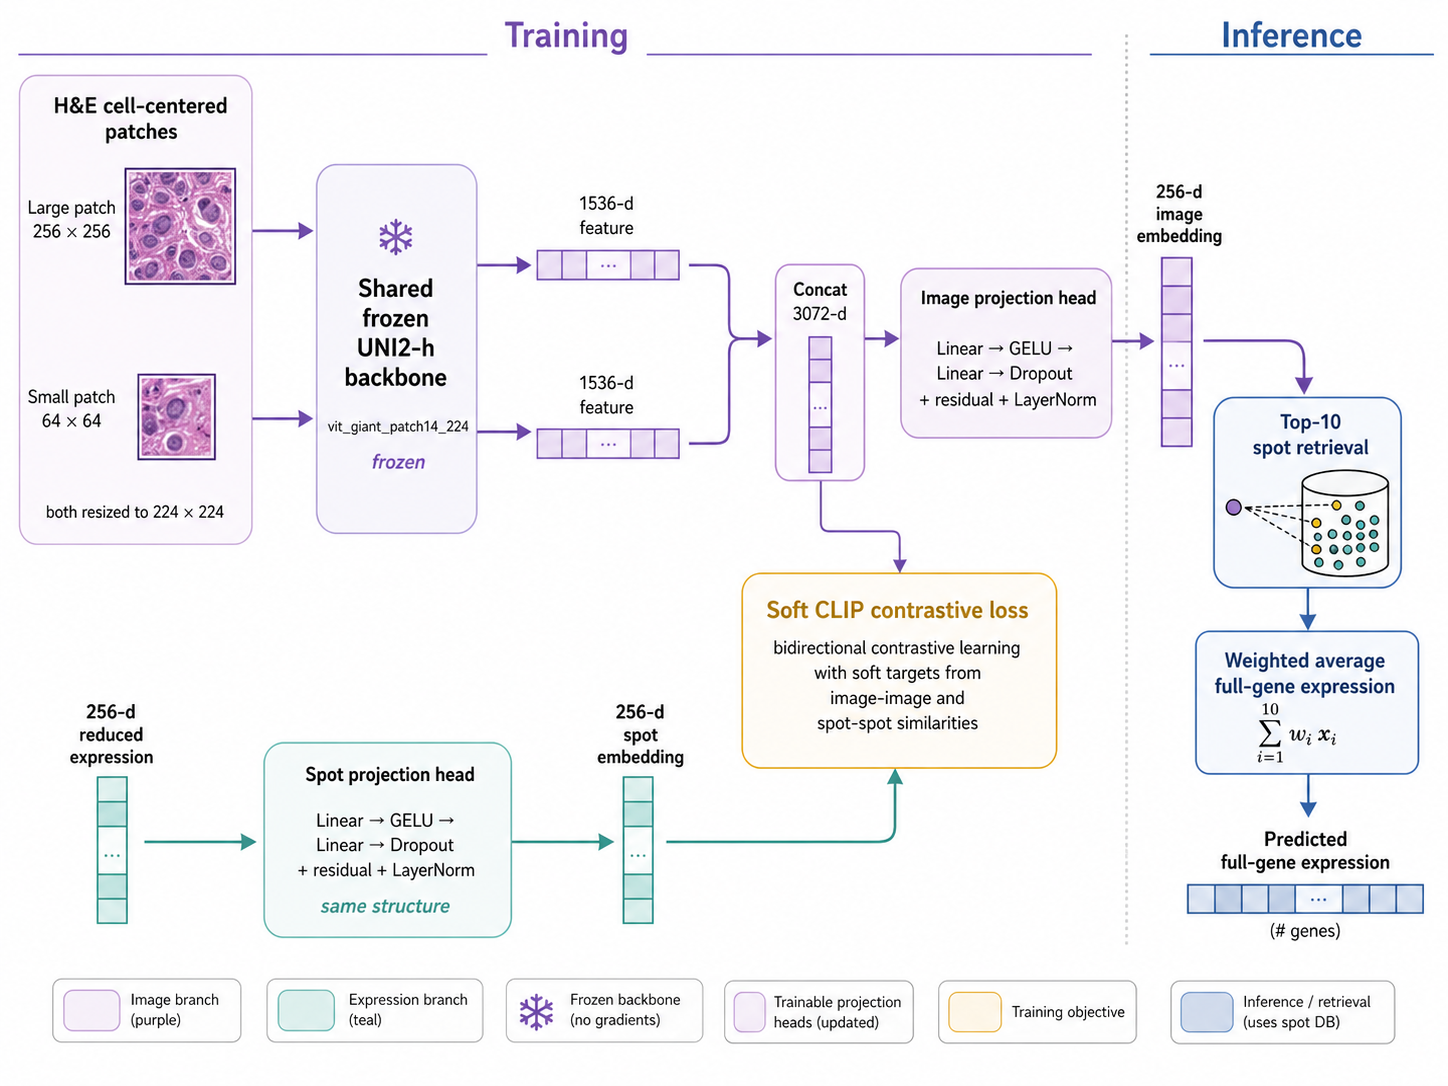
\includegraphics[width=0.8\linewidth]{model.png}
\caption{STBoost framework overview used for the appendix. A lightweight organ router selects an organ-specific expert, while paired cell-level and tissue-context crops are encoded, fused, and aligned to expression targets for downstream single-cell gene-expression prediction.}
\label{fig:appendix_model_overview}
\end{figure}

\noindent\textbf{Hierarchical encoder and fusion.}
Each expert uses a shared multi-scale image encoder $E_v(\cdot)$ together with a residual projection head $P_v(\cdot)$. The cell crop and tissue-context crop are first encoded separately,
\begin{align}
z_c &= E_v(I_c), & z_t &= E_v(I_t), \\
m &= W_2(\mathrm{GELU}(W_1[z_c; z_t])) + W_1[z_c; z_t], \\
h_v &= P_v([z_c; z_t]) = \mathrm{LayerNorm}(m).
\end{align}
This design keeps the local cell morphology and the broader microenvironment visible to the model at the same time. To explicitly couple local and contextual cues, STBoost further applies a cross-attention module that lets tissue-context tokens query the cell-level features:
\begin{equation}
\begin{aligned}
Q &= z_t W_Q, \quad K = z_c W_K, \quad V = z_c W_V, \\
\tilde{z}_t &= \mathrm{Softmax}\!\left(\frac{QK^\top}{\sqrt{d}}\right)V, \\
z_{\mathrm{fused}} &= \alpha \tilde{z}_t + (1-\alpha) z_t,
\end{aligned}
\end{equation}
where $\alpha$ is a learnable gating coefficient. The intuition is that ambiguous local morphology can borrow information from the surrounding tissue organization, while cells with strong intrinsic visual cues can remain dominated by their own aligned crop.

\noindent\textbf{Diffusion-based regularization.}
To keep predictions biologically smoother and less sensitive to high-frequency noise, STBoost uses a denoising-diffusion-style regularizer on the predicted expression output. Let $\epsilon\sim\mathcal{N}(0,I)$ and let $\hat{g}=f_{\theta_o}(I_c,I_t)$. The diffusion term is
\begin{equation}
\mathcal{L}_{\mathrm{diff}} =
\mathbb{E}_{t,\epsilon}\!
\left[
\left\lVert
\epsilon - \epsilon_\theta\!\left(\sqrt{\alpha_t}\hat{g}+\sqrt{1-\alpha_t}\epsilon,t\right)
\right\rVert_2^2
\right].
\end{equation}
This regularizer encourages manifold consistency between predicted outputs and the smoother structure expected from real biological expression states, reducing overfitting to noise and isolated artifacts.

\noindent\textbf{Training objective and loss design.}
Each expert is trained with a composite loss
\begin{equation}
\mathcal{L}=\lambda_1\|\hat{g}-g\|_1 + \lambda_2\mathcal{L}_{\mathrm{diff}} + \lambda_3\mathcal{L}_{\mathrm{align}},
\end{equation}
where $g$ is the target cell-level expression vector. The first term is the direct reconstruction loss, which keeps the model grounded in per-cell prediction accuracy. The alignment term $\mathcal{L}_{\mathrm{align}}$ is an InfoNCE contrastive loss that encourages paired image-derived and expression-derived embeddings to share a representation space while pushing apart mismatched pairs. The diffusion term provides a second level of regularization by penalizing predictions that leave the smoother biological manifold. Together, these terms balance pointwise reconstruction, multimodal alignment, and biologically motivated regularization.

\paragraph{Pilot structure and loss ablations.}
We further evaluate which components of the STBoost interface contribute most under a controlled pilot-scale setting. All variants are compared on the same A$\to$A protocol with matched training/reference cells, held-out test cells, preprocessing, target genes, and evaluation metrics. Structure ablations remove either the cell-centered crop or the broader histology-context branch, while loss ablations compare the default soft contrastive objective with hard or single-branch alternatives. Table~S8 summarizes the resulting trade-offs. Overall, the full STBoost interface provides the strongest balance across retrieval and regression metrics, whereas removing either image scale or simplifying the loss generally weakens cell-level image-to-gene alignment.

\begin{table*}[t]
\centering
\scriptsize
\setlength{\tabcolsep}{4pt}
\caption{STBoost pilot ablations on the A$\to$A protocol. All variants use $n_{\mathrm{train/ref}}=4096$ and $n_{\mathrm{test}}=2000$ under a matched pilot-scale evaluation budget, with identical preprocessing, split construction, target genes, and metrics.}
\label{tab:STBoost_k2k_ablation}
\resizebox{\linewidth}{!}{%
\begin{tabular}{l l l r r r r r r r r}
\toprule
\textbf{Variant} & \textbf{Image Branch} & \textbf{Loss Mode} & \textbf{Best Val Loss} & \textbf{$A\!\rightarrow\!A$ F1} & \textbf{Gene-Sp.} & \textbf{Cell-Sp.} & \textbf{Pred Rate} & \textbf{$\Delta$ Val} & \textbf{$\Delta$ F1} & \textbf{$\Delta$ Cell-Sp.} \\
\midrule
\texttt{full} & both & \texttt{soft\_clip} & 3.2920 & 0.1159 & 0.0386 & 0.1026 & 0.0728 & 0.0000 & 0.0000 & 0.0000 \\
\texttt{no\_cell\_patch} & \texttt{large\_only} & \texttt{soft\_clip} & 3.3064 & 0.1102 & 0.0498 & 0.1114 & 0.1180 & 0.0144 & -0.0057 & 0.0088 \\
\texttt{no\_image\_patch} & \texttt{small\_only} & \texttt{soft\_clip} & 3.7126 & 0.1173 & 0.0472 & 0.0981 & 0.0854 & 0.4206 & 0.0014 & -0.0045 \\
\texttt{hard\_clip} & both & \texttt{hard\_clip} & 3.2853 & 0.1159 & 0.0386 & 0.1026 & 0.0728 & -0.0067 & 0.0000 & -0.0000 \\
\texttt{spot\_only\_soft} & both & \texttt{spot\_only\_soft} & 2.4706 & 0.0802 & 0.0295 & 0.0983 & 0.1701 & -0.8214 & -0.0358 & -0.0043 \\
\texttt{image\_only\_soft} & both & \texttt{image\_only\_soft} & 4.0496 & 0.1193 & 0.0464 & 0.1039 & 0.0801 & 0.7576 & 0.0034 & 0.0013 \\
\bottomrule
\end{tabular}%
}
\end{table*}

The pilot yields three practical takeaways. First, the full model remains the best balanced default: it does not minimize every single metric, but it avoids the large calibration or validation penalties seen in the ablated variants. Second, \texttt{hard\_clip} is almost indistinguishable from the full \texttt{soft\_clip} run, so the current gains do not appear to depend strongly on that clipping choice. Third, the branch and loss ablations expose clear trade-offs rather than a single uniformly dominant simplification: removing the cell crop increases cell-wise Spearman to 0.1114 but lowers F1 and sharply increases predicted nonzero rate, removing the larger context crop hurts validation fit most among the structural variants, \texttt{spot\_only\_soft} achieves the lowest validation loss but the weakest F1, and \texttt{image\_only\_soft} slightly improves F1 only at the cost of much worse validation loss.

\noindent\textbf{Inference pipeline.}
For an unseen WSI, the full STBoost pipeline proceeds in three stages: (1) classify the WSI or sample context into an organ domain using $C(\cdot)$; (2) select the routed organ-specific expert $f_{\theta_{\hat{o}}}$; and (3) predict expression vectors for aligned cells using the paired local/context crops at each coordinate. This yields dense cell-level and tissue-level expression maps while keeping the same architecture across organs. By coupling a shared framework with domain-specific experts, STBoost provides a scalable and interpretable reference system for multi-organ histology-to-gene prediction.

\noindent\textbf{Relation to the reported benchmark tables.}
The 25-category breadth result in \Cref{tab:breadth_25} is the completed
multi-organ STBoost evaluation reported in the main paper. It uses the same
spatially buffered splits, training-only gene selection, and evaluation metrics
across all categories. The remaining appendix tables provide complementary
transfer, sensitivity, and ablation analyses under the released benchmark
protocol.

\subsection{Benchmark protocol details}
\label{sec:benchmark_protocol}
The current appendix reports the three benchmark regimes used throughout the paper: \textbf{in-domain}, \textbf{cross-patient}, and \textbf{cross-platform}. In-domain evaluation uses a left--right spatial split within a sample, with the left two thirds of the tissue used as the retrieval/reference bank and the right one third used as held-out evaluation. For the representative Visium HD sample A this split is implemented by an $x$-axis cutoff at 15,600.65 in full-resolution coordinates; for native-Xenium lung target X1 the corresponding cutoff is 1,933.71. Cross-patient evaluation keeps the same preprocessing and model protocol but changes the test sample, e.g., A$\!\rightarrow\!$B. Cross-platform evaluation changes both sample and acquisition technology, and is therefore restricted to the shared-gene set after gene-symbol harmonization.

The current appendix should be read as a matched three-regime benchmark package. Throughout the appendix, all reported retrieval results follow the same in-domain, cross-patient, and cross-platform protocol with shared preprocessing, target definitions, and evaluation code.

\subsection{Prediction targets and metric definitions}
\label{sec:prediction_metrics}
Two target definitions are used. Within-platform Visium HD runs use the full 18,085-gene panel available in the processed HD cell table. Cross-platform runs use only the shared genes between the train and test domains after harmonized symbol matching. In the completed experiments this yields 465 genes for A$\!\rightarrow\!$X2 and 370 genes for A$\!\rightarrow\!$X1 and X1$\!\rightarrow\!$B, while native-Xenium in-domain evaluation on X1 uses its 541-gene panel.

We report the same metric bundle for every completed run: nonzero-detection F1, nonzero-rate difference, gene-wise rank Spearman, cell-wise rank Spearman (reported as transposed rank Spearman), matrix distance, energy distance, and RBF-MMD. Gene-wise and cell-wise Spearman are averaged over the evaluation genes/cells respectively. F1 and rate difference summarize sparsity recovery, while the distribution metrics quantify broader mismatch even when sparse support looks reasonable.

\subsection{Pathology encoder benchmark protocol}
\label{sec:encoder_protocol}
The strongest completed frozen-encoder configuration in this revision uses the UNI2-h pathology encoder under a matched retrieval protocol. Each cell is represented by paired local/context crops with sizes 64 and 256 pixels, resized to the encoder input size of 224. The backbone is frozen, features are extracted once, and prediction is done with top-$k$ retrieval using $k=10$. For the Xenium$\leftrightarrow$Visium cached cross-platform experiments, the same retrieval logic is reused on cached features, together with shared-gene normalization on the expression targets. This is the protocol underlying the appendix benchmark analyses.

\subsection{Extended results for gene expression prediction}
\label{sec:extended_prediction_results}
\noindent
The appendix retrieval results are organized under the three standardized regimes. Two patterns are already clear. First, in-domain performance is consistently stronger than transfer, especially on the cell-wise Spearman metric. Second, cross-platform transfer remains heterogeneous: A$\!\rightarrow\!$X2 is meaningfully better than A$\!\rightarrow\!$X1, which is close to failure despite using the same encoder family and normalization recipe. This is exactly the kind of regime-specific behavior that motivated the benchmark.
\noindent
To make support explicit, \Cref{tab:organ_gene_cell_coverage} summarizes the
sample and cell coverage of the 25 release categories. It is a release-level
support view; the corresponding organ-wise performance results are reported
in the main paper.

\begin{table}[!t]
\centering
\scriptsize
\setlength{\tabcolsep}{2.2pt}
\renewcommand{\arraystretch}{0.98}
\caption{Release coverage across 25 organ categories, aggregated from
\Cref{tab:all_xenium_visium_summary}. Counts are aligned cells in the release,
not benchmark performance scores.}
\label{tab:organ_gene_cell_coverage}
\begin{tabularx}{\columnwidth}{
>{\raggedright\arraybackslash}p{1.60cm}
>{\raggedright\arraybackslash}X
>{\centering\arraybackslash}p{0.58cm}
>{\raggedleft\arraybackslash}p{1.05cm}}
\toprule
\textbf{Organ} & \textbf{Platform} & \textbf{N} & \textbf{Cells} \\
\midrule
Bone & Xenium & 1 & 253,560\\
Brain & Visium HD + Xenium & 4 & 986,867\\
Breast & Visium HD + Xenium & 6 & 2,613,649\\
Cervical & Xenium & 1 & 840,387\\
Colon & Xenium & 1 & 219,797\\
Colorectal & Visium HD + Xenium & 2 & 1,067,810\\
Embryo & Visium HD & 2 & 828,383\\
Head & Visium HD & 1 & 54,251\\
Heart & Xenium & 1 & 26,366\\
Kidney & Visium HD + Xenium & 5 & 866,399\\
Liver & Xenium & 1 & 239,271\\
Lung & Visium HD + Xenium & 6 & 1,328,335\\
Lymph Node & Visium HD + Xenium & 2 & 782,240 \\
Ovarian & Visium HD + Xenium & 4 & 1,497,900\\
Ovarian glands & Xenium & 1 & 1,157,659\\
Pancreas & Visium HD + Xenium & 3 & 696,358\\
Pancreatic & Xenium & 1 & 190,965\\
Pancreatic duct gland & Xenium & 1 & 235,099\\
Plant & Visium HD & 1 & 58\\
Prostate & Visium HD + Xenium & 2 & 392,766\\
Seed & Visium HD & 1 & 8,566\\
Skin & Xenium & 3 & 268,526\\
Small Intestine & Visium HD & 1 & 181,224\\
Tonsil & Visium HD + Xenium & 3 & 2,999,419\\
Xenograft & Visium HD & 1 & 263,743\\
\bottomrule
\end{tabularx}
\end{table}

\begin{figure}[t]
\centering
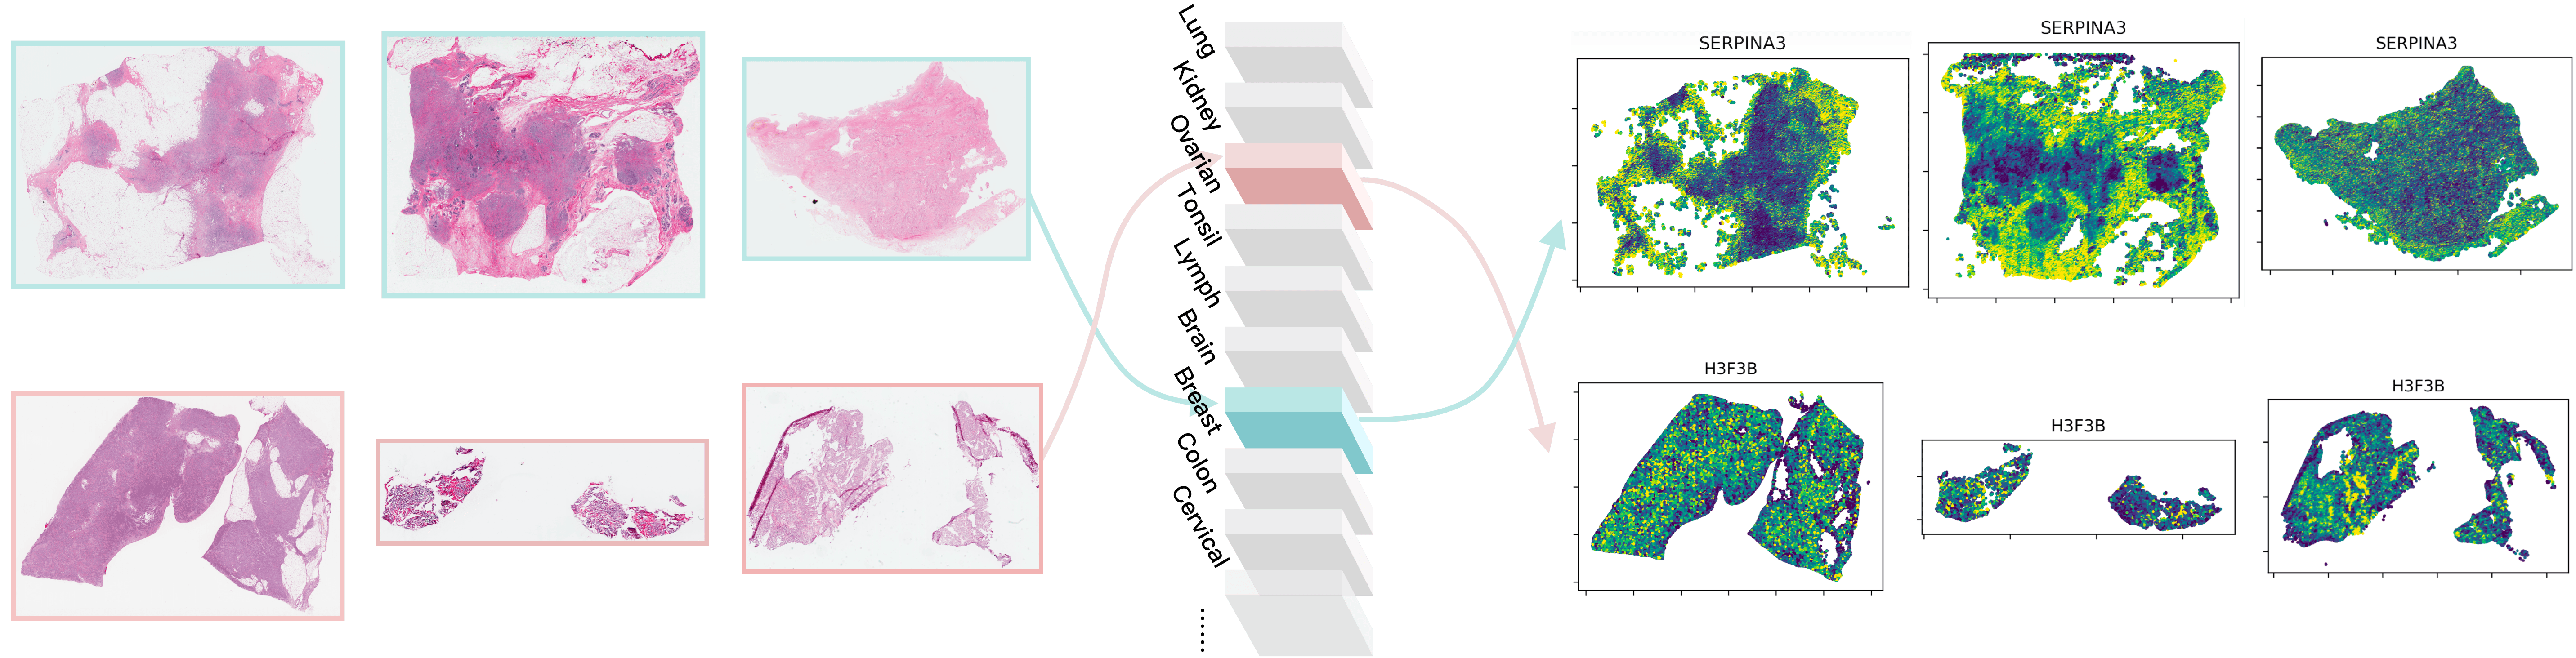
\includegraphics[width=1.0\linewidth]{exp2any.png}
\caption{TCGA whole-slide image qualitative test for STBoost. This panel illustrates what happens when TCGA WSI images are fed into the model, highlighting the kinds of spatial gene-expression patterns the framework can and cannot recover under this out-of-distribution evaluation setting.}
\label{fig:retrieval_qualitative_transfer}
\end{figure}

\subsection{Failure analysis and robustness notes}
\label{sec:failure_robustness}
The qualitative lesson from the completed runs is that transfer difficulty is not monotonic in platform alone. A$\!\rightarrow\!$X2 produces a usable shared-gene signal, while A$\!\rightarrow\!$X1 collapses on both F1 and rank-based correlation. This asymmetry suggests that study-specific acquisition, tissue state, or panel composition still dominate simple platform labels. The benchmark should therefore be interpreted as a stress test for realistic generalization rather than a leaderboard on a single homogeneous target.

\FloatBarrier

\subsection{Additional downstream analyses and use cases}
\label{sec:downstream_use_cases}
Beyond the core image-to-gene benchmark, \dataset supports analyses of coarse
cell state, tissue routing, and language-aligned records. These studies are
grouped here because they demonstrate possible uses of the released record
structure; none is treated as a primary benchmark claim.

\subsubsection{Coarse cell-state recovery}
\label{sec:coarse_cell_state}
Beyond direct gene retrieval, we also evaluated a coarse downstream celltype analysis on representative Visium HD lung sample A using the completed coarse-to-fine checkpoint. This analysis contains 111,772 cells, 10 unsupervised clusters, and a 50-gene target subset. Because this illustrative run uses a restricted 50-gene panel, only three marker-derived classes remain stable in the current appendix: \textit{Club}, \textit{AT2}, and \textit{Immune}. In other words, this is best read as a marker-derived coarse cell-state analysis rather than a full cell ontology benchmark.

\begin{figure*}[t]
\centering
\includegraphics[width=0.98\linewidth]{celltype.jpg}
\caption{Downstream celltype appendix panel for representative sample A. The panel summarizes whole-slide organization, local patch comparisons, and marker-derived celltype structure under the aligned cluster palette used throughout the downstream analysis.}
\label{fig:celltype_panel}
\end{figure*}

\begin{table}[t]
\centering
\scriptsize
\caption{Global metrics for the representative sample-A downstream celltype analysis.}
\label{tab:celltype_global}
\begin{tabular}{lc}
\toprule
\textbf{Metric} & \textbf{Value} \\
\midrule
Cells & 111,772 \\
Clusters & 10 \\
Genes in downstream target & 50 \\
GT vs. Pred celltype accuracy & 0.5935 \\
GT vs. Pred balanced accuracy & 0.5922 \\
Cluster vs. Pred celltype ARI & 0.1362 \\
Cluster vs. Pred celltype NMI & 0.2154 \\
Retained marker-derived classes & Club, AT2, Immune \\
\bottomrule
\end{tabular}
\end{table}

\begin{table*}[t]
\centering
\scriptsize
\setlength{\tabcolsep}{5pt}
\caption{Cluster-level summary for the representative sample-A downstream analysis after aligning the out-of-sample cluster colors to the global cluster palette. Agreement is the fraction of cells in the cluster with matching GT-derived and prediction-derived coarse celltype labels.}
\label{tab:celltype_cluster_summary}
\begin{tabular}{c r l c l c c}
\toprule
\textbf{Cluster} & \textbf{\# cells} & \textbf{Dominant GT} & \textbf{GT frac.} & \textbf{Dominant Pred} & \textbf{Pred frac.} & \textbf{Agreement} \\
\midrule
0 & 26,397 & Club & 0.660 & Club & 0.695 & 0.639 \\
1 & 3,778 & Immune & 0.519 & Immune & 0.509 & 0.474 \\
2 & 13,542 & Immune & 0.720 & Immune & 0.798 & 0.656 \\
3 & 7,067 & Club & 0.958 & Club & 0.966 & 0.934 \\
4 & 9,922 & AT2 & 0.541 & AT2 & 0.657 & 0.516 \\
5 & 10,219 & Immune & 0.472 & Immune & 0.520 & 0.460 \\
6 & 9,073 & AT2 & 0.609 & AT2 & 0.736 & 0.574 \\
7 & 20,349 & Club & 0.514 & Club & 0.532 & 0.550 \\
8 & 9,299 & AT2 & 0.489 & AT2 & 0.574 & 0.488 \\
9 & 2,126 & Immune & 0.712 & Immune & 0.768 & 0.670 \\
\bottomrule
\end{tabular}
\end{table*}

\subsubsection{Multi-organ classification}
\label{sec:multi_organ_classification}

\noindent
This subsection is kept as a reference-model implementation detail rather than as a core benchmark contribution. When organ routing is used in a full-model pipeline, it determines which organ-specific expert is invoked before gene prediction. False positives mostly increase compute cost, whereas false negatives can route a patch to the wrong expert family and hurt downstream prediction quality.

We trained and tested our multi-class classifier with the PanNuke Dataset, a nuclei segmentation and classification dataset from histopathology images. The dataset importantly consists of nearly 8,000 square tissue patches with $256\times256$ pixel resolution across 19 different tissue types, including various cancerous and non-cancerous tissues.

For the classifier, we utilized a 2D Convolutional Neural Network (CNN) with an EfficientNetB0 backbone pretrained on ImageNet. The performance is summarized using precision, recall, F1-score, and prediction accuracy.

The model achieved an overall accuracy of $88.84\%$, with a macro-precision of $0.8947$, a macro-recall of $0.8879$, and a macro-F1 of $0.888$. As shown in Table~\ref{tab:organ_classification}, per-class performance is consistently strong across the 19 PanNuke tissue classes, with the main errors arising from morphologically similar organs such as bile duct and liver. We therefore keep this result in the appendix as supporting evidence that organ routing is feasible when a reference pipeline needs it.

\begin{figure}[t]
\centering
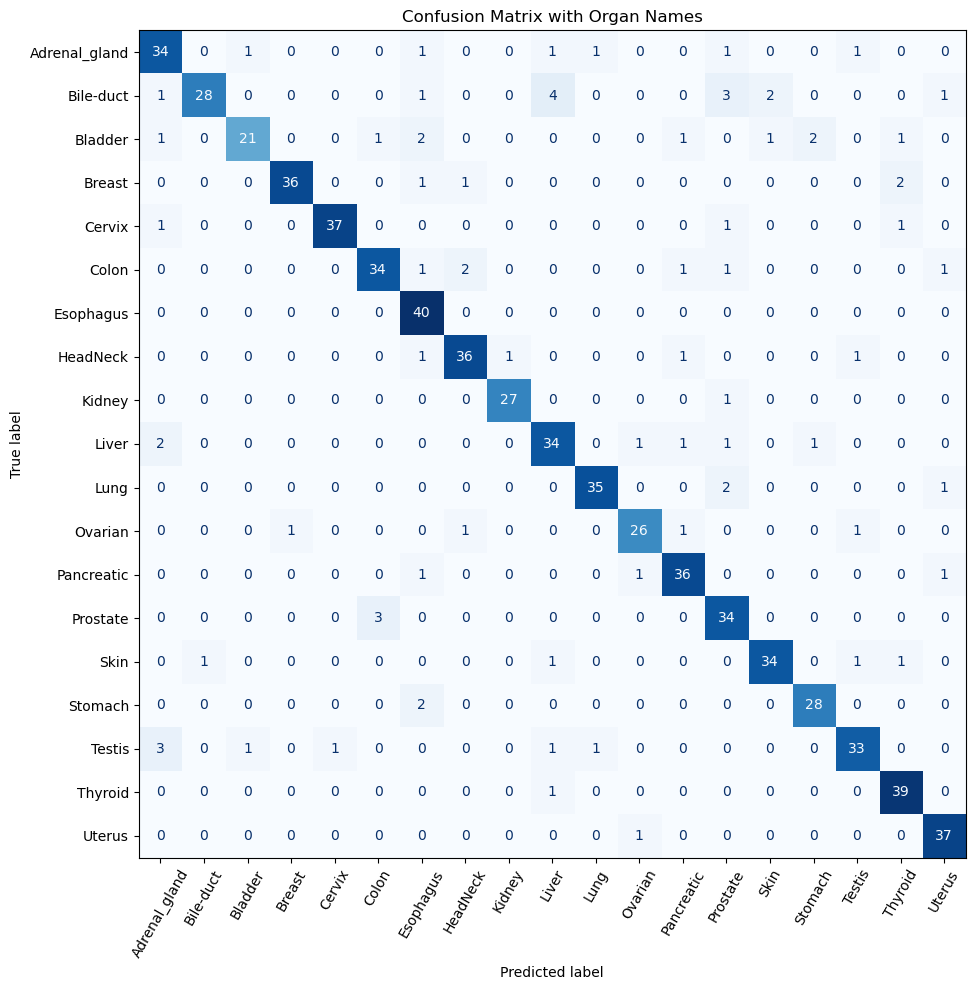
\includegraphics[width=0.6\linewidth]{Multi-Organ_Classification_Results.png}
\caption{Confusion matrix for the multi-organ classifier. Most mass remains on the diagonal, with the largest residual confusion concentrated among morphologically similar tissue classes.}
\label{fig:organ_classification_confusion}
\end{figure}

\begin{table}[t]
\centering
\scriptsize
\setlength{\tabcolsep}{6pt}
\begin{tabular}{lcccc}
\toprule
\textbf{Class} & \textbf{Precision} & \textbf{Recall} & \textbf{F1-score} & \textbf{Support} \\
\midrule
Adrenal\_gland & 0.81 & 0.85 & 0.83 & 40 \\
Bile-duct      & 0.97 & 0.70 & 0.81 & 40 \\
Bladder        & 0.91 & 0.70 & 0.79 & 30 \\
Breast         & 0.97 & 0.90 & 0.94 & 40 \\
Cervix         & 0.97 & 0.93 & 0.95 & 40 \\
Colon          & 0.89 & 0.85 & 0.87 & 40 \\
Esophagus      & 0.80 & 1.00 & 0.89 & 40 \\
HeadNeck       & 0.90 & 0.90 & 0.90 & 40 \\
Kidney         & 0.96 & 0.96 & 0.96 & 28 \\
Liver          & 0.81 & 0.85 & 0.83 & 40 \\
Lung           & 0.95 & 0.92 & 0.93 & 38 \\
Ovarian        & 0.90 & 0.87 & 0.88 & 30 \\
Pancreatic     & 0.88 & 0.92 & 0.90 & 39 \\
Prostate       & 0.77 & 0.92 & 0.84 & 37 \\
Skin           & 0.92 & 0.89 & 0.91 & 38 \\
Stomach        & 0.90 & 0.93 & 0.92 & 30 \\
Testis         & 0.89 & 0.82 & 0.86 & 40 \\
Thyroid        & 0.89 & 0.97 & 0.93 & 40 \\
Uterus         & 0.90 & 0.97 & 0.94 & 38 \\
\midrule
Accuracy       & ---  & ---  & 0.89 & 708 \\
Macro Avg      & 0.89 & 0.89 & 0.89 & 708 \\
Weighted Avg   & 0.89 & 0.89 & 0.89 & 708 \\
\bottomrule
\end{tabular}
\caption{Per-class classification performance on the organ recognition task.}
\label{tab:organ_classification}
\end{table}

\subsubsection{Caption generation and semantic-consistency audit}
\label{sec:caption_audit}
\noindent
Captioning remains an auxiliary modality in the current release rather than a main benchmark target. We keep it because structured text can help browse the data package and support future multimodal work, but we do \emph{not} treat caption quality as evidence that language is central to the current gene-prediction benchmark.

The caption pipeline is grounded primarily in metadata and image-derived context rather than unconstrained free-form generation. Metadata fields such as organ, platform, and local spatial context are used to construct the prompt context, and quality control is performed with image-text similarity checks rather than manual claims about biological correctness. In the current appendix we therefore report captioning conservatively, as a release feature and auxiliary validation tool, not as a core performance result.

To make the relevance claim concrete, we include a combined PLIP+CONCH diagnostic figure. The upper part summarizes PLIP-based sample-level image--caption similarity, while the lower part summarizes CONCH-based organ/image-directory similarity using $k=10$ captions per organ. Taken together, these views show that the metadata-grounded captions are not arbitrary text strings: matched image--caption pairs generally score higher than mismatched pairs at both the sample and organ levels, even though captioning remains an auxiliary release feature rather than a benchmark headline result.

\begin{table}[t]
\centering
\small
\setlength{\tabcolsep}{3.2pt}
\caption{\textbf{Image--caption semantic-consistency audit.} Matched pairs
refer to the paired image--caption entries in the original similarity
matrices. Top-$k$ accuracy records whether the matched caption is retrieved
among an image's $k$ most similar candidates.}
\label{tab:image_caption_alignment}
\begin{tabular}{@{}lrrrr@{}}
\toprule
Model & Matched / other & Enrichment & AUC & Top-1 / Top-3 \\
\midrule
PLIP  & .262 / .053  & $4.96\times$ & .993 & 84.6\% / 100\% \\
CONCH & .040 / .0021 & $19.1\times$ & .988 & 90.9\% / 100\% \\
\bottomrule
\end{tabular}
\end{table}

The table quantifies the positive alignment visible in
Figure~\ref{fig:caption_similarity_human}: both independently trained
pathology vision--language models rank the paired captions substantially above
mismatched captions. However, a separate leakage audit also exposes an
important limitation. Among 1,070 readable generated captions, every caption
explicitly contained the supplied cell-type label; after literal removal of
that label, the remaining text still recovered the label with 0.999 accuracy
and 0.996 macro-F1. We therefore release captions only as optional,
label-conditioned derived artifacts. They are useful for data browsing and
multimodal method development, but they are not an independent factual
validation target and are not used by the primary image-to-gene benchmark.
Future caption versions should be evaluated with a label-blind prompt and an
independent human factuality audit.

\begin{figure}[!t]
\centering
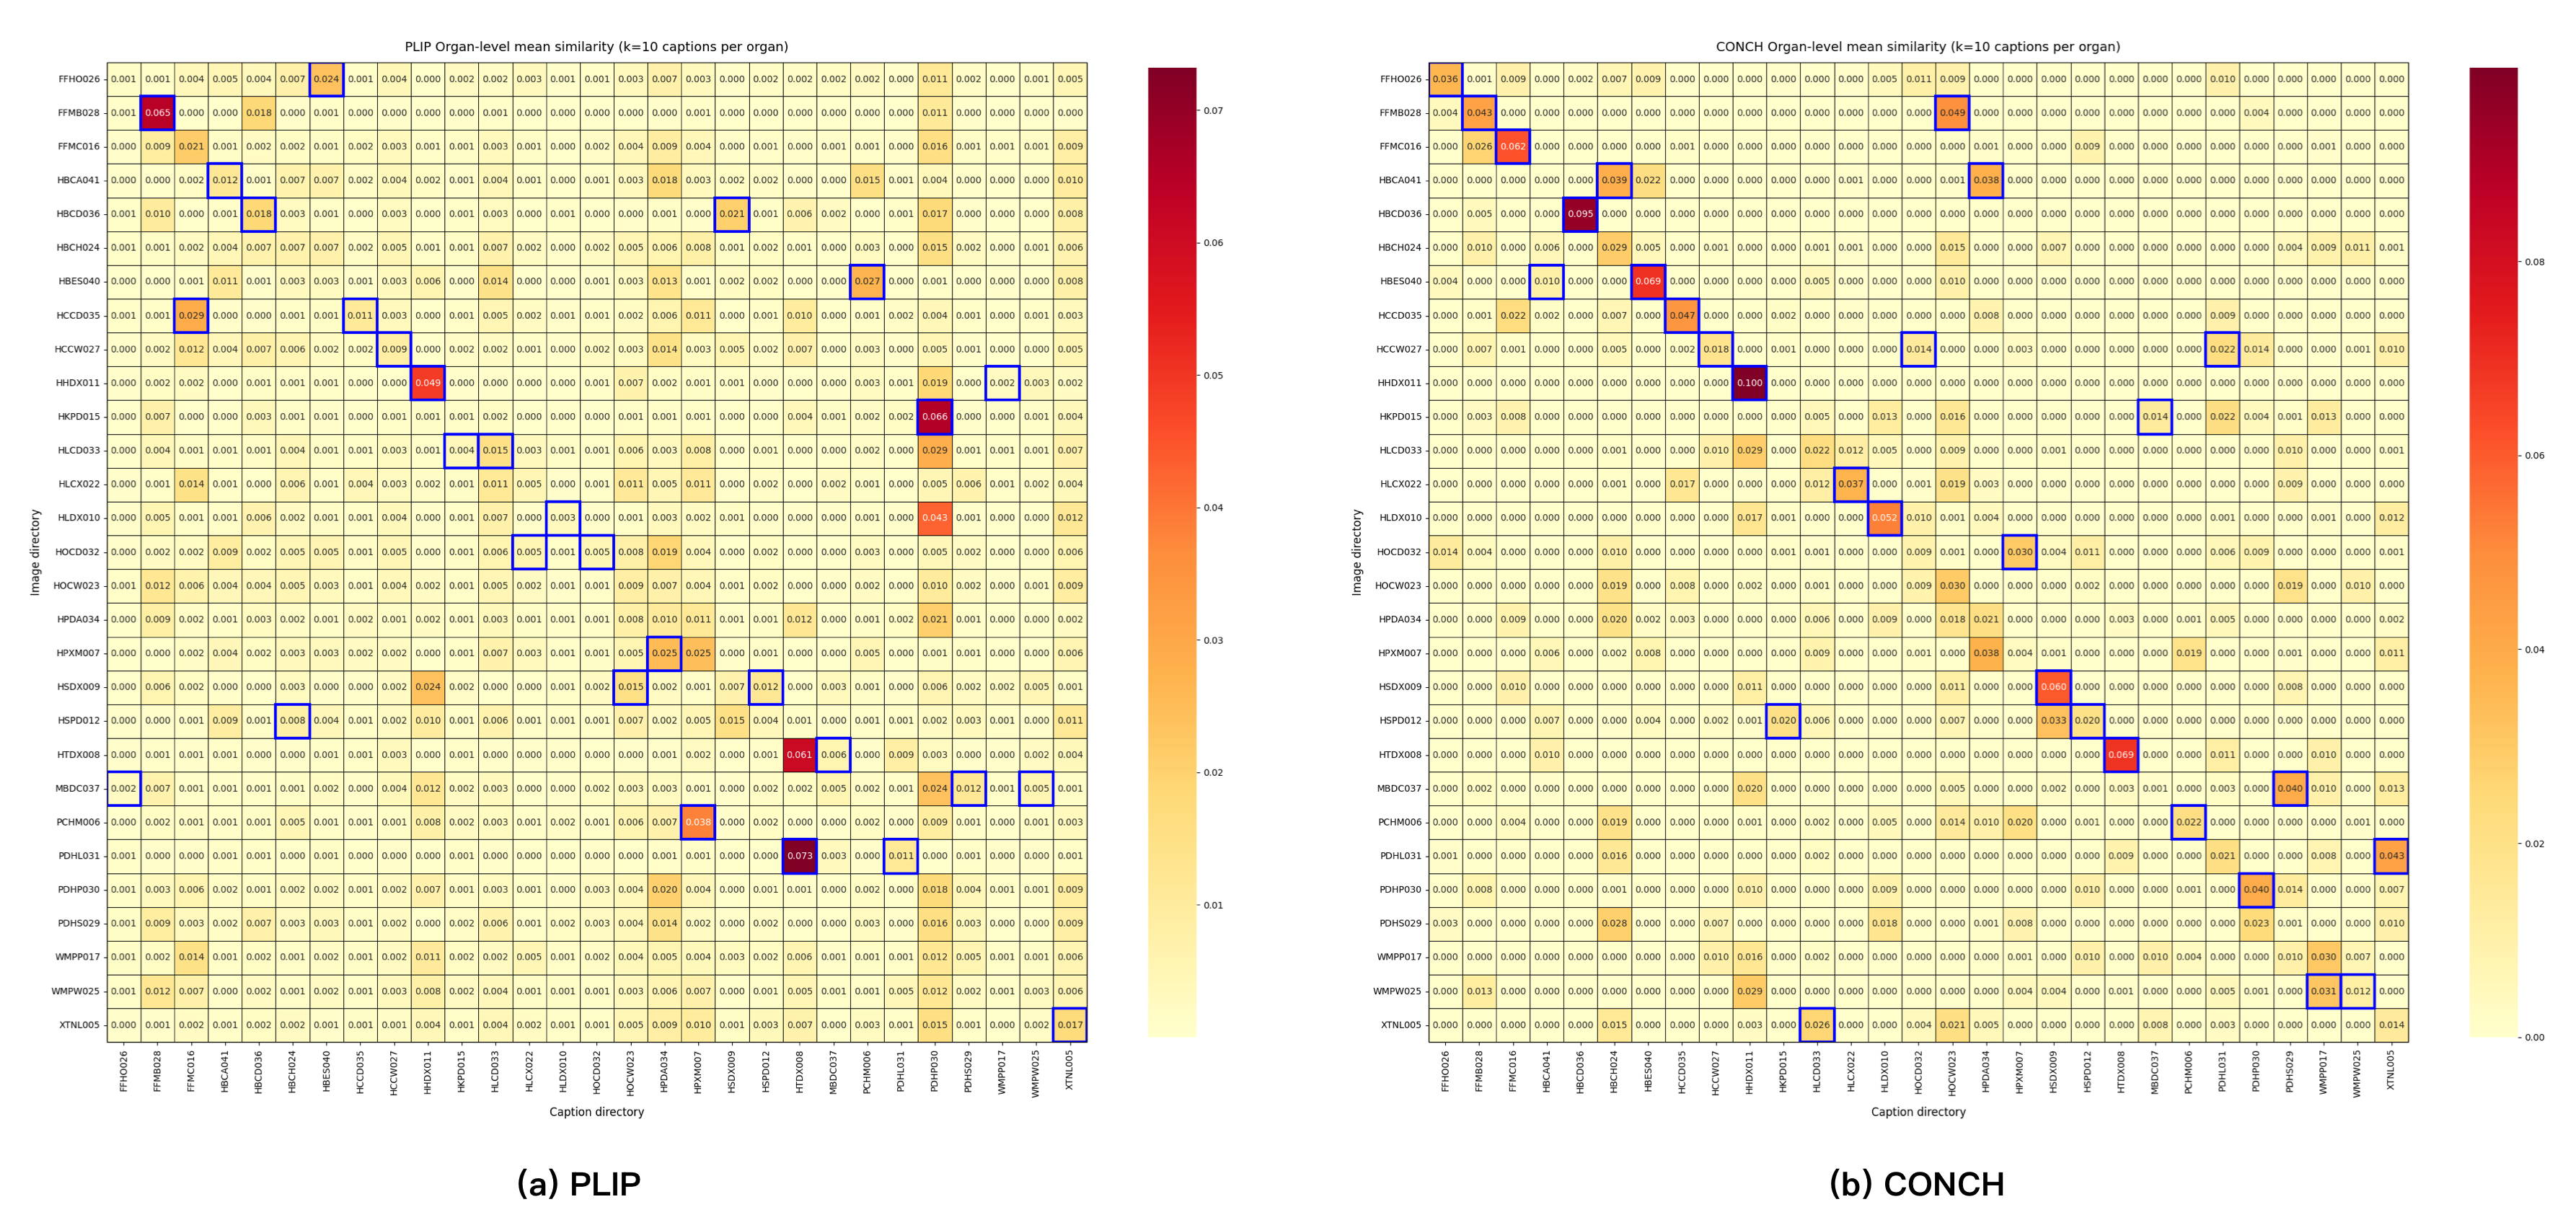
\includegraphics[width=0.98\linewidth]{plip_conch.png}
\caption{\textbf{PLIP and CONCH caption-relevance diagnostics.}
The PLIP sample-level and CONCH organ-level similarity matrices provide two
independent views of image--caption alignment. Quantitative matched-versus-
mismatched summaries are reported in
\Cref{tab:image_caption_alignment}.}
\label{fig:caption_similarity_human}
\end{figure}

\FloatBarrier

\section{Datasheet for \dataset}
\label{sec:cellnet_datasheet}
\noindent
We provide a DataSheet for \textbf{\dataset}, summarizing its objectives, scope, and design choices, along with potential applications and ethical considerations.
The datasheet below emphasizes the benchmark-facing aspects of the release: the unit of analysis is the aligned cell, benchmark tracks are defined through explicit split files, and the released schema is versioned so that the same processed assets can be used for both modeling and evaluation.

\subsection{Motivation for dataset creation}
\datasheetq{Why was the dataset created?}
\dataset is a large-scale single-cell dataset featuring paired imaging and gene expression data, with multi-level imaging modalities that capture detailed cellular structures. This comprehensive multimodal resource incorporates elements such as captioning, CCC (cell-cell communication), and attribute annotations, creating a rich interconnected framework. Moreover, \dataset serves as a versatile benchmark for foundation models, broadening the scope of existing case studies and facilitating research across multiple tissues and modalities.

\begin{itemize}
    \item \textbf{Extensive Single-Cell Dataset:} Provides a vast collection of paired image and gene expression data, capturing cellular characteristics at multiple layers and scales.
    \item \textbf{Multimodal Content:} Integrates captioning, cell-cell communication (CCC), attribute annotations, and multi-tier imaging, enabling deeper insights into phenotypic and molecular interrelationships.
    \item \textbf{Benchmark Utility:} Offers a foundational platform for evaluating and enhancing current models, expanding potential applications and analytical perspectives across tissues and modalities.
\end{itemize}
\datasheetq{What tasks could the dataset be used for?}
Potential tasks include cross-modal retrieval, cell-type classification, morphological phenotype analysis, spatial domain segmentation, and gene expression prediction from histology images. Users are welcome to devise new applications but are strictly prohibited from attempting to re-identify patients.

\datasheetq{Has the dataset been used for any tasks already?}
Yes. The current study demonstrates utility in cross-modal retrieval and few-shot cell typing, among others (\S4). Researchers can refer to the main paper for baselines and performance metrics.

\datasheetq{Who funded the creation of the dataset?}
\dataset was developed with institutional support from multiple sources; details are provided in the Acknowledgments section of the main manuscript.

\dataset Bench is intended to provide predefined splits, target definitions, and evaluation scripts for single-cell histology-to-gene prediction under standardized regimes. The benchmark is therefore not only a collection of multimodal data, but also a controlled evaluation package with fixed preprocessing and explicit held-out partitions.

%--------------------------------------------------------------------------------------

\subsection{Dataset composition}
\datasheetq{What are the instances?}
Instances in \dataset are \textit{single-cell} samples, each associated with:
\begin{itemize}
    \item Three hierarchical image patches (cell-level, tissue-level, WSI-level).
    \item Gene expression profiles and structured metadata.
    \item Textual captions describing morphological and contextual details.
    \item Cell-cell communication profiles.
\end{itemize}

\datasheetq{Are relationships between instances made explicit?}
Yes. Each cell is uniquely mapped to its corresponding gene expression vector, tissue type, and spatial coordinates. Cell-to-cell communication edges (ligand-receptor pairs) are also provided, capturing local interactions within a 200\,$\mu$m radius.

\datasheetq{What does each instance consist of?}
\begin{itemize}
    \item \textbf{Imaging data:} Standard TIFF patches at cell, tissue, and WSI scales.
    \item \textbf{Expression data:} CSV or HDF5 files storing normalized read counts for thousands of genes.
    \item \textbf{Metadata:} JSON or CSV containing cell type, disease state, organ, and additional attributes (e.g., \texttt{Position\_in\_WSI}).
    \item \textbf{Captions:} Automated textual descriptions of morphological features and context.
\end{itemize}

\datasheetq{Is there a label/target associated with instances?}
Each cell is linked to a variety of annotations (e.g., \texttt{cell\_type}, \texttt{cell\_disease\_state}). Demographic information is partially available (for certain human samples) and subject to IRB and licensing constraints.

\datasheetq{Are external resources required?}
All data are released as part of \dataset; external links to original publications are included in the metadata. Each source dataset is licensed in a manner that permits downstream distribution and derivative works.

\datasheetq{Recommended data splits or evaluation measures?}
Yes. We provide recommended splits (train/val/test) for tasks such as gene-expression prediction and morphological classification. These splits are included as CSV files within the repository.

\datasheetq{What experiments were initially run on this dataset?}
Our main paper details multiple experiments, including cross-modal retrieval (image$\leftrightarrow$gene) and spatial domain segmentation. Please refer to the Results section for a comprehensive discussion.

Benchmark metadata makes the release directly executable. Each retained cell is associated with study, sample, platform, organ, and spatial-coordinate fields; benchmark tracks record whether the cell belongs to in-domain, cross-patient, or cross-platform evaluation; and review subsets preserve the same schema as the full release even when only lightweight assets are mirrored during anonymous review.

%--------------------------------------------------------------------------------------

\subsection{Data collection process}
\datasheetq{How was the data collected?}
\dataset aggregates single-cell data primarily from 10x Genomics (Xenium \& Visium HD) and in-house experiments. Each study provides histopathology images, transcriptomic profiles, and relevant sample metadata.

\datasheetq{Who was involved?}
All authors of this paper contributed to data curation and validation. Original acquisition protocols (e.g., IRB approvals, tissue preparation) are documented in the source publications.

\datasheetq{Over what time frame was the data collected?}
The dataset spans public studies published between 2016 and 2025, along with ongoing additions as new data become available.

\datasheetq{Is the dataset a sample from a larger set?}
We aim to include all single-cell data from the selected studies. Instances are unique pairings of morphological patches and expression profiles. Minor omissions may arise if crucial alignment files are missing.

\datasheetq{Known errors or sources of noise?}
Whole-slide images vary in quality due to staining differences, compression artifacts, and resolution limits. Gene expression data may exhibit batch effects or sequencing noise. Users are encouraged to apply standard normalization/denoising procedures as needed.

Studies were included only when both histology and spatial-molecular coordinates were available and could be aligned at cell level. Samples lacking reliable coordinate transforms, segmentation support, or sufficient image coverage were excluded from benchmark construction. Repeated sections are handled at the sample/split level so that duplicated material does not leak across the realized benchmark partitions.

%--------------------------------------------------------------------------------------

\subsection{Data preprocessing}
\datasheetq{What preprocessing was done?}
\begin{itemize}
    \item \textbf{Image processing:} All slides converted to pyramidal TIFF, with standardized pixel resolutions.
    \item \textbf{Gene expression standardization:} Data stored in uniform formats (Scanpy objects, CSV) with consistent gene labeling.
    \item \textbf{Cell-level alignment:} Each cell’s bounding box and expression profile carefully cross-validated to ensure correct mapping.
\end{itemize}

\datasheetq{Were raw data retained?}
Original raw files are stored offline for certain in-house studies. Public re-download links are provided for public samples. The repository hosts processed data for immediate use.

\datasheetq{Is preprocessing software available?}
Yes. The code for generating multi-scale patches and gene expression transformations is available in the \textbf{\dataset GitHub repository} at \url{https://anonymous.4open.science/r/sMMC-22M-dataset-ED70}.

For the benchmark tracks reported in this appendix, preprocessing is fixed rather than tuned per method. Retrieval experiments use paired 64-pixel and 256-pixel crops resized to 224 for the encoder; Visium HD uses processed cell-level expression derived from native 2\,$\mu$m bins; Xenium uses platform cell tables or cached features; and communication summaries use a 200\,$\mu$m neighborhood definition. Shared-gene cross-platform benchmarks are computed from the processed release itself, not from hidden internal files, so the released assets are sufficient to reproduce the reported tables.

%--------------------------------------------------------------------------------------

\subsection{Dataset distribution}
\datasheetq{How is the dataset distributed?}
All data (images, expression files, metadata, tutorials) are hosted on GitHub:
\begin{center}
\url{https://anonymous.4open.science/r/sMMC-22M-dataset-ED70}
\end{center}

\datasheetq{When will it be released?}
\dataset is publicly accessible as of this study’s publication. Interested users can clone or download it following the README instructions.

\datasheetq{Under what license?}
The processed release is distributed under the license stated in the
repository. Public source data retain their original study- and
portal-specific terms; users must comply with both the release license and the
corresponding upstream terms.

\datasheetq{Who maintains the dataset?}
The dataset is actively maintained by the authors. For questions or inquiries, please submit an issue on the GitHub page.

\datasheetq{Will the dataset be updated?}
Yes. We plan periodic updates as new single-cell samples are curated. Dataset versioning will track changes, documented via GitHub releases.

The benchmark release includes split CSV/JSON files, benchmark configs, evaluation scripts, plotting utilities, and model-loading examples in the repository. Because the full processed dataset is substantially larger than the lightweight review package, the anonymous release prioritizes scripts, metadata summaries, and representative benchmark assets that preserve the same schema and protocol used by the full package.

%--------------------------------------------------------------------------------------

\subsection{Legal and ethical considerations}
\datasheetq{Ethical review approvals?}
All in-house data adhere to institutional IRB protocols. Public data rely on the ethical compliance of the original sources. Detailed references to each study’s IRB are included where available.

\datasheetq{Could this dataset expose individuals to harm?}
No patient identifiers (name, address, etc.) exist in \dataset. Users are strictly forbidden from attempting re-identification or reverse engineering of personal data.

\datasheetq{Sensitive or offensive content?}
No. The dataset focuses on cellular-level data and lacks personal or demographic attributes aside from basic clinical labels (e.g., \texttt{cancer} vs. \texttt{healthy}).

\datasheetq{Social bias or fairness concerns?}
Demographic fields are available only when supplied by the source study, and
their coverage is incomplete and uneven. Models trained on the release may
therefore inherit demographic, study, disease, or platform biases. The context
fields support stratified audits, but they do not by themselves establish
population representativeness or fairness.

\datasheetq{Licensing fees or restrictions?}
No fees. The data must be used according to the terms of the open-source license. Commercial usage may require additional permissions.

\datasheetq{Future updates or obsolescence?}
If the dataset is ever discontinued, we will note this in the GitHub README. We encourage the community to mirror or fork the repository for long-term availability.

Benchmark scores should not be interpreted as uniformly representative across all biological domains. Organ, species, and platform coverage are deliberately broad but highly uneven, and demographic metadata are sparse for many public studies. The benchmark is therefore best understood as a reproducible stress test for multimodal pathology models, not as a clinically calibrated estimate of performance for any individual population.

\balance
\section{Author Statement}
\label{sec:author_statement}
\noindent
The authors bear responsibility for the curation, processing, documentation,
and release decisions associated with \dataset.

\section{Reproducibility Checklist for \dataset Bench}
\label{sec:reproducibility_checklist}
\noindent
To reproduce the appendix benchmarks, a user needs the processed cell-level release, the split files for the chosen regime, and the corresponding evaluation script. The essential checklist is:
\begin{itemize}
    \item the benchmark environment file and package versions used by the released scripts;
    \item the processed cell tables and aligned image crops for the selected subset;
    \item split CSV/JSON files defining in-domain, cross-patient, and cross-platform partitions;
    \item evaluation scripts for retrieval, cross-platform plotting, and downstream celltype analysis;
    \item the random seed and job configuration used for any training or feature-cache generation;
    \item sufficient local storage for cached features and figure outputs.
\end{itemize}

In practice, the appendix results reported here can be regenerated directly from the processed benchmark assets and scripts already referenced throughout this document. The three-regime benchmark package described in this appendix uses the same processed release, split definitions, and evaluation scripts throughout.

\end{document}
